\documentclass[12pt, twoside]{report}
	\usepackage[margin=1in]{geometry}
	\usepackage[hidelinks, linktoc=all, pagebackref]{hyperref}
	\usepackage{indentfirst}
    \usepackage{subcaption}
   	\usepackage[superscript,biblabel]{cite}
    \usepackage[font=small,labelfont=bf]{caption}
    \usepackage{abstract}
    \usepackage{mathtools}
    \usepackage{mathrsfs}  
    \usepackage{cleveref}
    \usepackage{fancyhdr}
    \usepackage{enumitem}
    \setlength{\parskip}{0.1cm}   
	\setlength{\parindent}{0.7cm}
    \usepackage{graphicx} % Used to insert images
    \usepackage{adjustbox} % Used to constrain images to a maximum size 
   	\usepackage{color} % Allow colors to be defined
    \usepackage{geometry} % Used to adjust the document margins
    \usepackage{amsmath} % Equations
    \usepackage{amssymb} % Equations
    \usepackage[mathletters]{ucs} % Extended unicode (utf-8) support
    \usepackage[utf8x]{inputenc} % Allow utf-8 characters in the tex document
    \usepackage{fancyvrb} % verbatim replacement that allows latex
    \usepackage{grffile} % extends the file name processing of package graphics 
                         % to support a larger range 
    % The hyperref package gives us a pdf with properly built
    % internal navigation ('pdf bookmarks' for the table of contents,
    % internal cross-reference links, web links for URLs, etc.)
    \usepackage{longtable} % longtable support required by pandoc >1.10
\usepackage{bbm}

\newcommand{\diff}{\,\mathrm{d}} 	
 \renewcommand{\figureautorefname}{Fig.}%
\renewcommand*\thesection{\arabic{section}}
\DeclarePairedDelimiter\bra{\langle}{\rvert}
\DeclarePairedDelimiter\ket{\lvert}{\rangle}
\DeclarePairedDelimiterX\braket[2]{\langle}{\rangle}{#1 \delimsize\vert #2}
\newcommand{\rbrkt}[1]{\left( #1 \right)}
\newcommand{\sbrkt}[1]{\left[ #1 \right]}

\renewcommand*{\backreftwosep}{ and~}
\renewcommand*{\backreflastsep}{ and~}
\renewcommand*{\backref}[1]{}
\renewcommand*{\backrefalt}[4]{%
\ifcase #1 %
\relax%
\or
(referenced on p. [#2])%
\else
(referenced on p. [#2])%
\fi
}

\numberwithin{equation}{section}
\setcounter{tocdepth}{3}

\renewcommand*\thesection{\arabic{chapter}.\arabic{section}}
\lhead[\rm\thepage]{\fancyplain{}{\nouppercase{\sl{\rightmark}}}}
\rhead[\fancyplain{}{\nouppercase{\sl{\leftmark}}}]{\rm\thepage}
\chead{}\lfoot{}\rfoot{}\cfoot{}
\pagestyle{fancy}

\title{Reverse engineering of the Xmon qubits}

\graphicspath{{Pictures/}, {MIPT NIR presentation/Pics/}}


\begin{document}
\maketitle
\tableofcontents

%\chapter{Theoretical introduction}

\section{Superconducting microwave coplanar waveguide resonators}

\subsection{Equations for quality factors}

The total quality factor of a microwave transmission line resonator (TLR) $Q_l$ (loaded quality factor) can be calculated as a sum of two parts -- the internal and external quality factors. The internal quality factor $Q_i$ describes how excitations leave the resonator in the absence of coupling to any external circuitry, so damping in this case comes from the internal defects (i.e., resonant two-level systems) in the resonator itself. When, however, the resonator is coupled to the external circuitry having some active resistance, the damping is enhanced and the total Q-factor is reduced according to the following expression:
\begin{equation}
Q_l^{-1} = Q_i^{-1}+Q_e^{-1},
\label{eq:qfactor}
\end{equation}
where $Q_e$ is determined by the value of the externally connected resistance and the way of its connection.

\begin{figure}
\captionsetup[subfigure]{width = 0.9\textwidth, justification=normal}
\centering
\begin{subfigure}[t]{0.48\textwidth}
\centering
\includegraphics[width=0.9\textwidth]{resonator}
\caption{Real world circuit configuration.}
\end{subfigure}
\begin{subfigure}[t]{0.48\textwidth}
\centering
\includegraphics[width=0.9\textwidth]{resonator_equiv}
\caption{Norton equivalent of (a).}
\end{subfigure}

\caption{Equivalent circuit for a $\lambda/4$ TLR, capacitively coupled to the transmission line near resonance.}
\label{fig:resonator_equiv}
\end{figure}

A common way of measuring a resonator is to couple it capacitively to an external transmission line. The coupling on the equivalent scheme of the circuit is represented as $C_\kappa$, as depicted in \autoref{fig:resonator_equiv}~(a). An infinite/properly terminated transmission line can be represented as a single resistance of $Z_0$ Ohms, where $Z_0$ is the line's wave impedance; thus, two such resistances are added to the both sides of the resonator circuit. The resonators are of $\lambda/4$ type, so the equivalent for each of them is a parallel RLC oscillator (see below), where $C$ and $L$ are, respectively, its equivalent capacitance and inductance and $R=R_{in}$ characterises the internal dissipation. Its $Q_i  = \omega_0 C R_{in}$ where $\omega_0 = \sqrt{1/LC}$ can be calculated from the definition when no external impedance is connected.
 
The external Q-factor can be derived in a bit more complicated way\cite{Goppl2008}. We can transform the circuit from the \autoref{fig:resonator_equiv}~(a) to explicitly include the external parameters into the internal ones. To do so one needs to convert the series connection of the coupling capacitor and the characteristic impedances into parallel, as done on the \autoref{fig:resonator_equiv}~(b). The $R^*$ and $C^*$ impedances should be chosen in such a way that total impedance of the external circuit is the same as before the transformation:
\begin{align}
R^{*} &= \frac{1+\omega^2 C_\kappa^2 (Z_0/2)^2}{\omega^2 C_\kappa^2 (Z_0/2)	}, \\
C^{*} &= \frac{C_\kappa}{1+\omega^2 C_\kappa^2 (Z_0/2)^2} \approx C_\kappa\ (\text{in our case}). \label{eq:C_ast}
\end{align}
From this and \autoref{fig:resonator_equiv}~(b) it is simple to write down the expression for the internal, external and loaded quality factors:
\begin{gather}
Q_i =  \omega (C+C^{*}) R_{in}, \\
Q_e = \omega (C+C^{*}) R^{*}, \\
Q_l = \omega (C+C^{*})  \frac{1}{1/R^{*}+1/R_{in}}. \label{eq:Q_l}
\end{gather}
The above expressions readily justify \eqref{eq:qfactor}. The values been used in the simulations are: $C = 350$ fF, $L = 2$ nH, $R_{in}=10^7$ Ohm, $Z_0 = 50$ Ohm. 


\begin{figure}
\centering
\includegraphics[width=0.9\textwidth]{q-factors}
\caption{Q-factors dependence on $C_\kappa$ according to \eqref{eq:Q_l}.}
\end{figure}


\subsubsection{The lumped-element model of a coplanar waveguide resonator}\label{ssec:LE-model}
A $\lambda/4$ coplanar waveguide (CPW) resonator near a resonance is equivalent to a lumped-element parallel resonance circuit, as in \autoref{fig:resonator_equiv}. $L$ and $C$ for the lumped-element models of CPW resonators are bound not only by the resonance frequency condition $\omega_0 = 1/\sqrt{LC}$ but also by the geometry of the waveguide or, in other words, $C^\prime$ and $L^\prime$ -- the transmission line capacitance and inductance per unit length. To show this, one would write down the impedance of the CPW resonator near its resonance frequency $\omega_0$ and compare it to the lumped-element one's\cite{pozar2012}. Such comparison leads to the following expressions:
\[
R_{in} = \frac{Z_0}{\alpha l}, \quad C = \frac{\pi}{4\omega_0 Z_0},
\]
where $l$ is the resonator length, $Z_0 = \sqrt{L^\prime/C^\prime}$ is the wave resistance and $\alpha$ is the decay constant of the line. Then the resonance condition for the wavelength ($\lambda = 4 l$) is used along with the phase velocity expression $v_{ph} = 1/\sqrt{L^\prime C^\prime}$:
\[
\omega_0 = \frac{2\pi v_{ph}}{\lambda} =  \frac{\pi \, v_{ph}}{2 l} \Rightarrow  C = \frac{C^\prime l}{2}.
\]
For the inductance one can use $L = 1/\omega_0^2 C = 8 l\, L^\prime/\pi^2$. Finally, the expressions for $C^\prime$ and $L^\prime$:
\[
C^\prime = 4\varepsilon_0\varepsilon_{eff} \frac{K(k_0)}{K(k_0^\prime)},\quad
L^\prime = \frac{\mu_0}{4} \frac{K(k_0^\prime)}{K(k_0)},
\]
where $K(x)$ is the complete elliptic integral of the first kind, $\varepsilon_{eff} = \frac{1+\varepsilon_{substrate}}{2}$, $k_0 = \frac{W}{W+2G}$ where $W$ is the width of the hotwire and $G$ is the width of the gaps and finally $k_0^\prime = \sqrt{1-k_0^2}$.

\subsection{S-parameters for lines with resonators}

Typically, a microwave device under test (DUT) is tested with a vector network analyser, which measures the scattering matrix (S-matrix) of the DUT. So below we will discuss the S-matrix for two different coupling configurations. Generally, a two-port DUT can be drawn like in \autoref{fgeneral2port}. For such system it is possible to calculate different 2 by 2 matrices, which bind together voltages and currents on the ports 1 and 2. S-matrix also has 4 values, named S-parameters.

\begin{figure}[h]
\centering
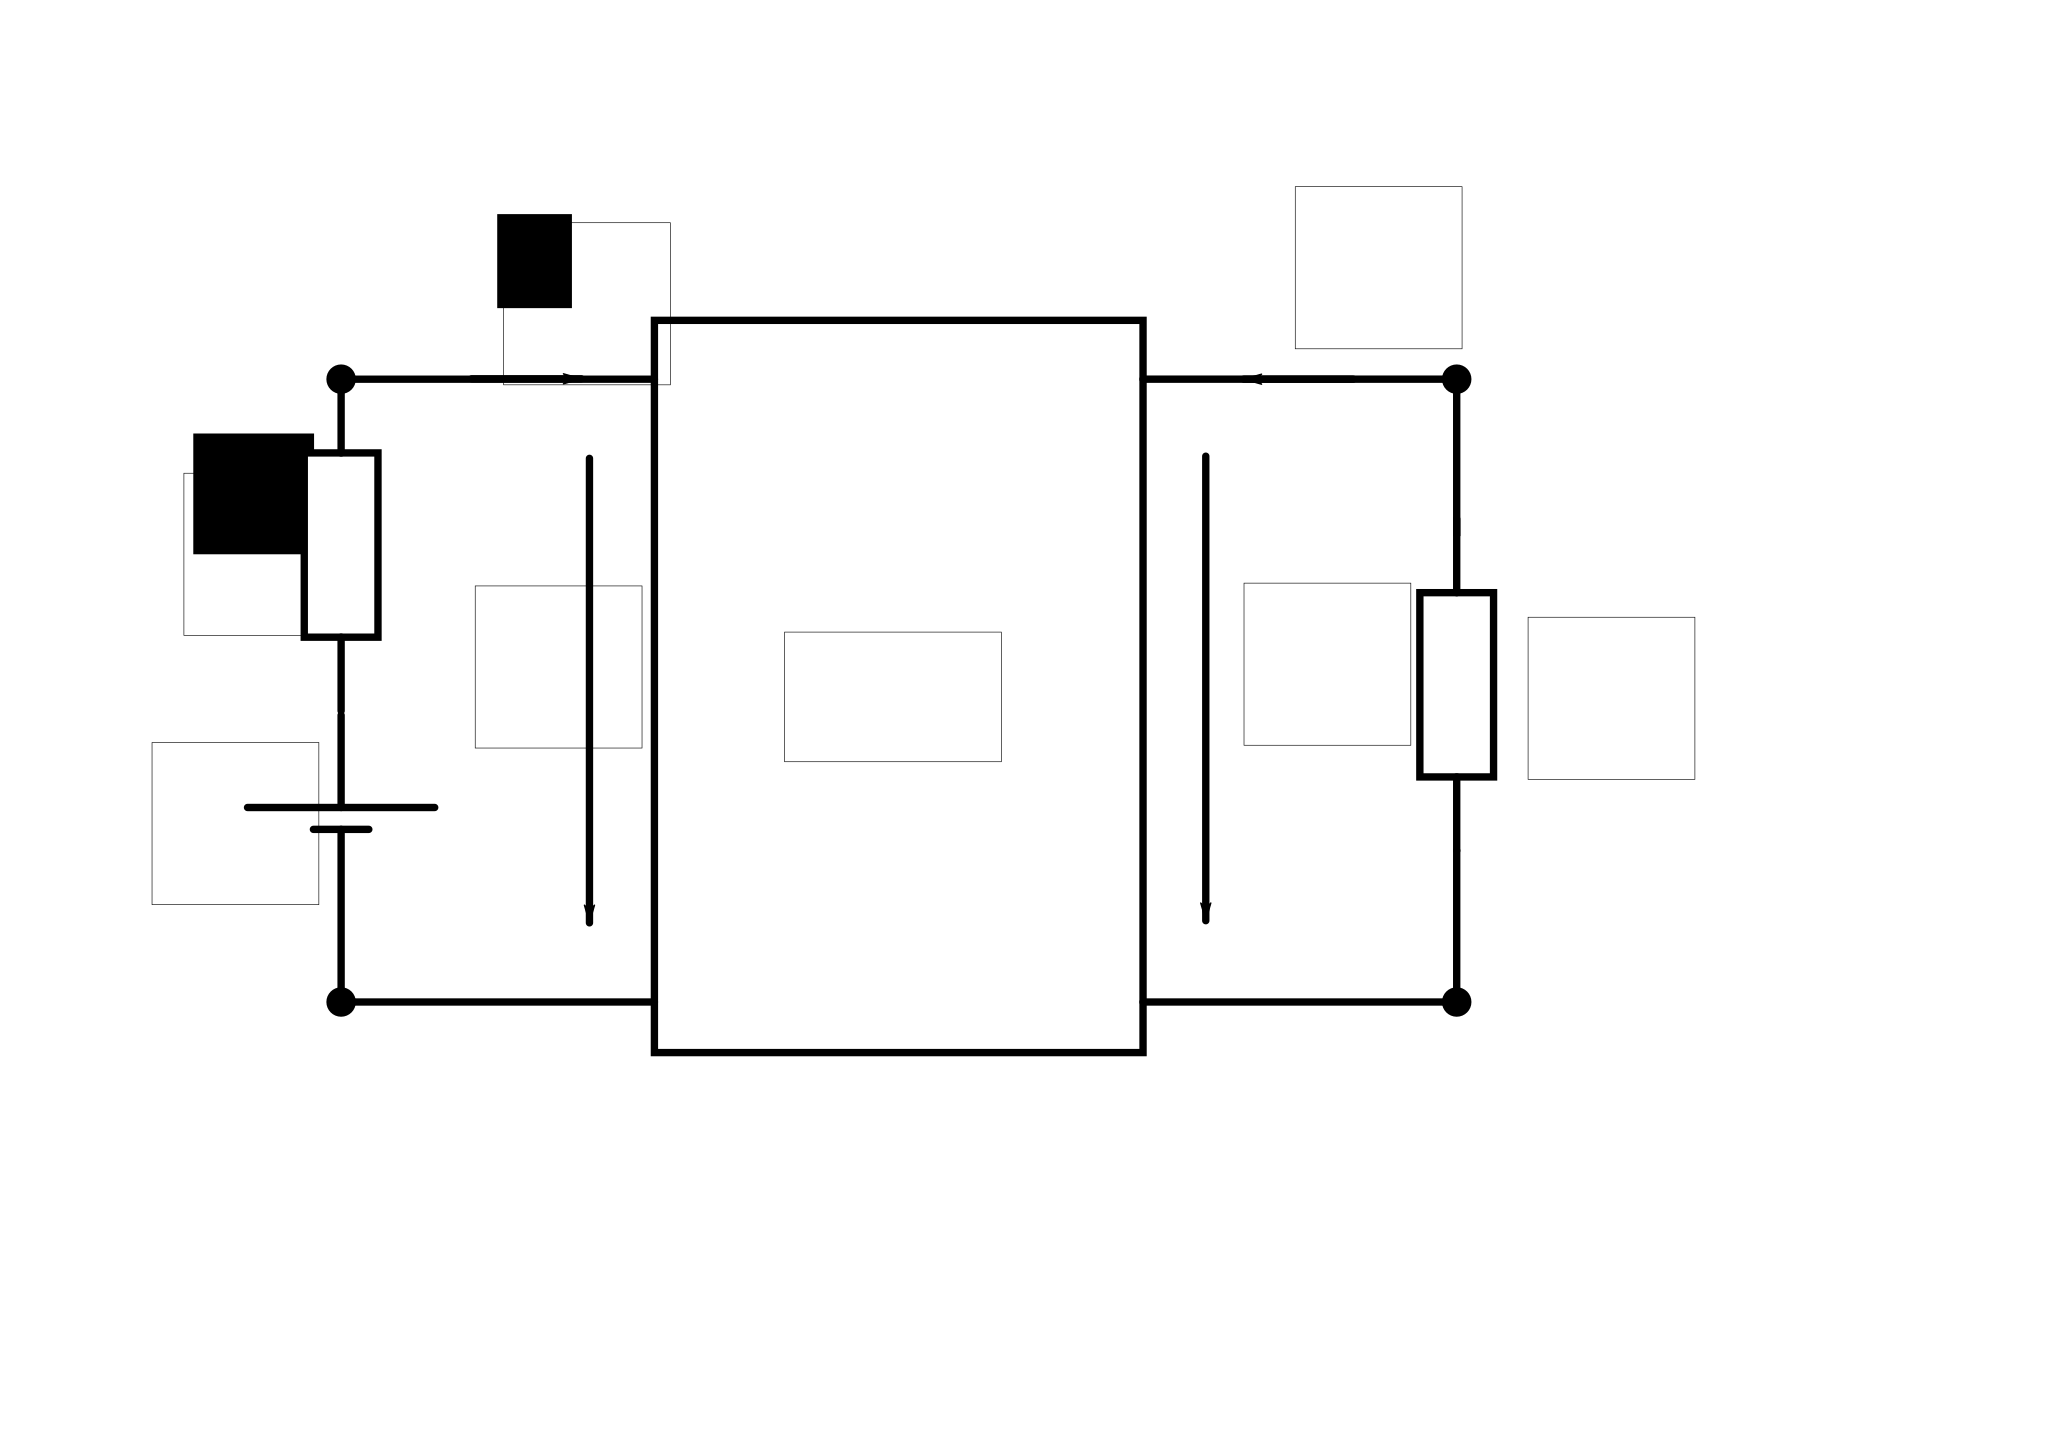
\includegraphics[width=0.5\textwidth]{tl_scheme_general}
\caption{A scheme for the two-port network.}
\label{fgeneral2port}
\end{figure}

To calculate S-parameters one needs to treat voltages and currents, which can be calculated from Kirchhoff's laws, as a sum of the incident and reflected components (``+'' corresponds to the incident wave and ``$-$'' to the reflected wave):
\begin{gather*}
V_{1,2} = V_{1,2}^+ + V_{1,2}^- ,\\
I_{1,2} = I_{1,2}^+ + I_{1,2}^- = \frac{ V_{1,2}^+ - V_{1,2}^- }{Z_0},
\end{gather*}
where the difference in the second expression arises from telegrapher's equations. Solving these with respect to incident and reflected components, one can get
\begin{equation*}
V_{1,2}^\pm = \frac{1}{2}(V_{1,2} \pm Z_0 I_{1,2}).
\end{equation*}
From this, finally, S-parameters are defined:
\begin{equation}
\rbrkt{\begin{matrix}
V_1^- \\
V_2^-
\end{matrix}} = 
\rbrkt{\begin{matrix}
S_{11} & S_{12} \\
S_{21} & S_{22}
\end{matrix}}
\rbrkt{\begin{matrix}
V_1^+ \\
V_2^+
\end{matrix}}.
\label{eq:S_def}
\end{equation}
However, it's often more convenient to use indirect methods of calculating S-parameters, for example, to extract them from $ABCD$-matrix.




\subsubsection{Notch (shunting) design}
For a notch design one can treat the resonator as a shunt in the transmission line as in \autoref{fig:shunted_tl}. Except than by the definition \eqref{eq:S_def} there are two other ways to calculate the S-matrix. First one is intuitive but is not valid for every configuration. Transmission and reflection parameters are defined\cite{Kiselev2013} below (the second formula is valid only for the ``shunt'' configuration, no series elements are allowed in the line):
\begin{gather}    
\Gamma = \frac{Z_{eff} - Z_{0}}{Z_{eff} + Z_{0}} = S_{11} = S_{22}, \label{eGamma}\\
T = \frac{2Z_{eff}}{Z_{eff}+Z_0} \overset{!}{=} S_{21} = S_{12}, \label{eT}
\end{gather}
where $Z_{eff} = Z_0 || Z_{shunt}$, $Z_{shunt} = \frac{1}{i\omega C_\kappa} + 1/i\omega C||R_{in}||i\omega L$ and the equalities between S-parameters hold due to the symmetry.
\begin{figure}[h]
\centering
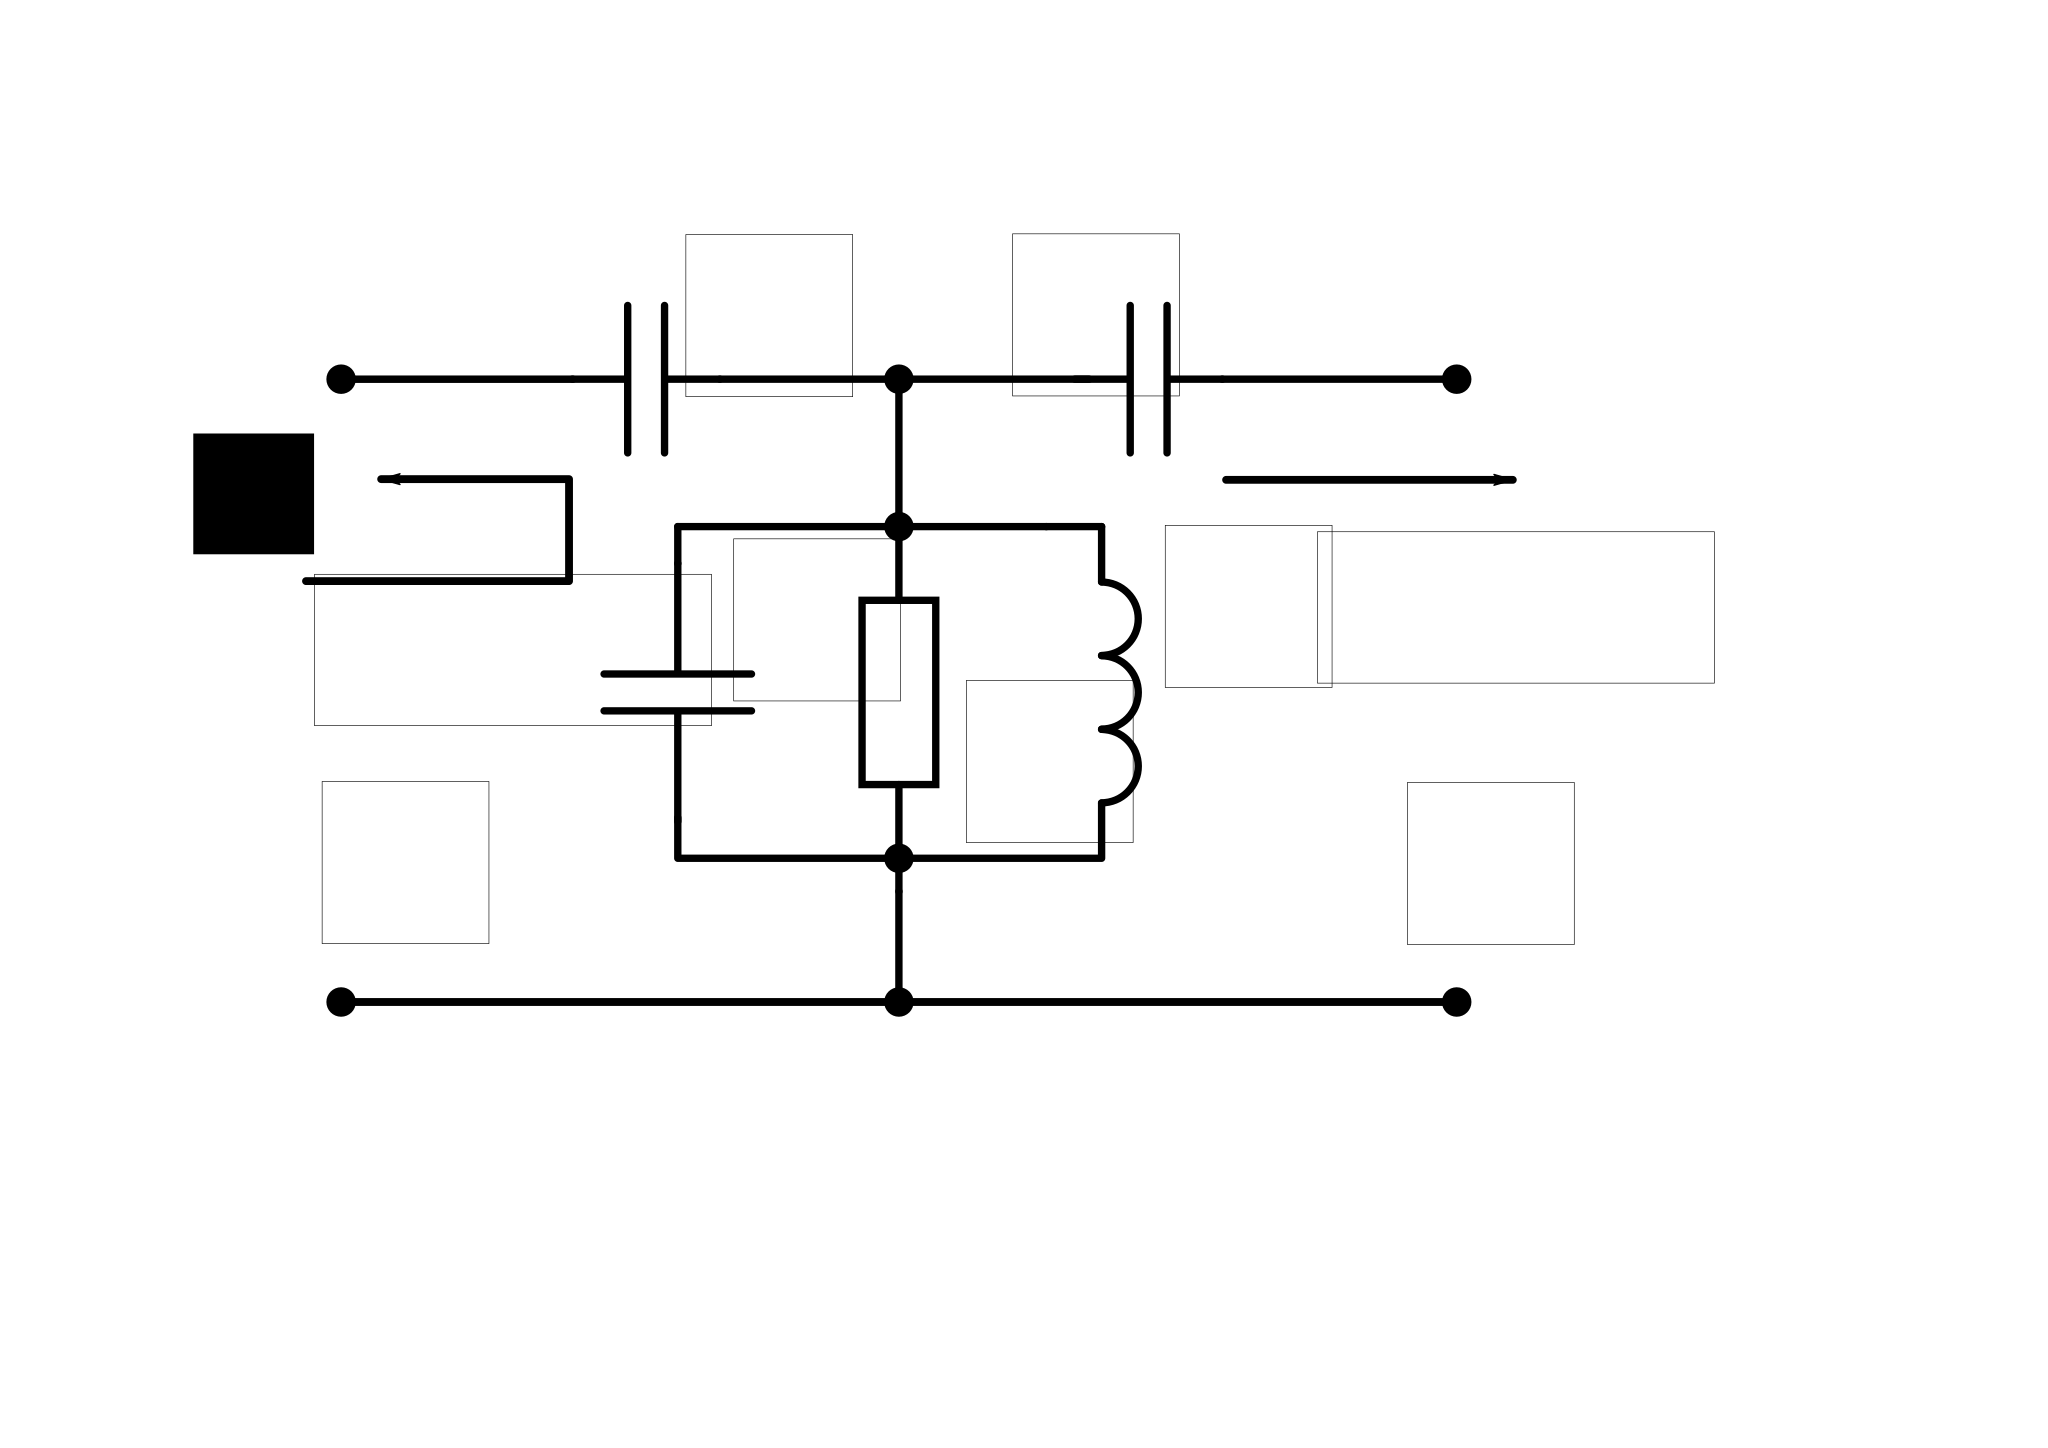
\includegraphics[width=0.5\textwidth]{tl_scheme}
\caption{The shunted transmission line. This is \autoref{fig:resonator_equiv}~(a)  from the observer's point of view.}
\label{fig:shunted_tl}
\end{figure}
\begin{figure}[h]
\centering
\includegraphics[width=0.99\textwidth]{S21s}
\caption{ $|S_{21}|$ parameters from \eqref{eq:S21} for different coupling strengths. The loaded quality factors are calculated with \eqref{eq:Q_l} and with the ``3db''-method. The red dashes show the values of expression $\sqrt{1/L(C+C_k)}$ according to \autoref{fig:resonator_equiv}~(b), the green ones show the theoretically predicted depths.}
\label{fig:S21s}
\end{figure}

Another way is to calculate $ABCD$ matrix or impedance matrix and convert it to the S-matrix with corresponding formulae\cite{pozar2012}. In the ``shunted'' case from both this approaches the simplified expressions for the S-parameters follow:
\begin{gather}
S_{11} = -\frac{Z_0}{1 + 2Z_{shunt}/Z_0} = S_{22}, \\
S_{21} = \frac{1}{1+Z_0/2Z_{shunt}} = S_{12}. \label{eq:S21}
\end{gather}
The second expression is plotted in \autoref{fig:S21s} along with the loaded quality factors calculated with \eqref{eq:Q_l} and with the ``3db''-method ($Q_L \approx \omega_0/\Delta\omega_{3db}$). It can be seen that with increase of capacitance resonance frequency and $Q_l$ decrease, which is expected according to \autoref{fig:resonator_equiv}~(b) and \eqref{eq:C_ast}.

In \autoref{fig:S21s} the resonance frequencies calculated from the equivalent circuit in \autoref{fig:resonator_equiv}~(b) are shown along with the analytically calculated depths of the peaks:
\begin{equation}
\min_f |S_{21}| = \frac{2 L \left(C + C_{\kappa}\right)}{\sqrt{C_{\kappa}^{2} L Z_{0}^{2} \left(C + C_{\kappa}\right) + \left(2 (C+C_\kappa) L + C_{k}^{2} R_{in} Z_{0} \right)^{2}}}.
\end{equation}

\subsubsection{Embedded (series) design}

For the embedded resonator it's possible to draw a similar equivalent circuit as for the ``shunt'' design\cite{Goppl2008}. It is depicted in \autoref{fseries_tl}. 

\begin{figure}[h]
\centering
\includegraphics[width=0.5\textwidth]{tl_scheme_series}
\caption{The equivalent circuit for the embedded resonator.}
\label{fseries_tl}
\end{figure}
\begin{figure}[h]
\centering
\includegraphics[width=0.9\textwidth]{S21s_series}
\caption{$S_{21}$ for the series configuration. Loaded Q-factors were calculated  via analytic expression similar to \eqref{eq:Q_l}.}
\label{fS21s_series}
\end{figure}

For this kind of connection of the resonator to the transmission line \eqref{eT} is now not valid (however, \eqref{eGamma} still holds). To calculate transmission in this case one may find the transmission matrix and then convert it to the S-matrix or use Kirchhoff's laws and \eqref{eq:S_def}. For studied case one can get the following $ABCD$-matrix\cite{pozar2012}
\begin{equation}
\hat T = \rbrkt{\begin{matrix}
A & B \\
C & D
\end{matrix}} = \rbrkt{\begin{matrix}
1 + \frac{1/i\omega C_\kappa}{Z_{res}} & 2/i\omega C_\kappa - \frac{\omega^2 C_\kappa^2}{Z_{res}} \\
1/Z_{res} &  1 + \frac{1/i\omega C_\kappa}{Z_{res}} 
\end{matrix}},
\end{equation}
where $Z_{res} = R_{in}||i\omega L || 1/i\omega C$. The corresponding $S_{21}$ is plotted in \autoref{fS21s_series}, calculated as\cite{pozar2012} 
\begin{equation}
S_{21} = \frac{2}{A+B/Z_0 +CZ_0 + D}.
\end{equation}

\subsection{Time-resolved response}

As soon as the spectral characteristics of the resonator are established, it is possible to calculate its response when a pulse of finite width is applied to it. The shape that the pulse will have after the interaction with the resonator is important when pulsed readout is considered in time-resolved qubit measurements. 

In this section we will only discuss the notch-type resonator and only the transmission of the pulses; however, the numerical method that will be used can be straightforwardly applied to other cases. It consists of three steps: calculate the discrete Fourier transform (DFT) for the input pulse, multiply it by the chosen complex S-parameter for each frequency (negative and positive frequencies should be multiplied in the same way), and finally perform the inverse DFT. 

We will use the following expression for the complex $S_{21}$ of an ideal notch-type resonator\cite{probst2015}:

\[
S_{21} (\omega)= 1 - \frac{Q_l/Q_e}{1 + 2 i Q_l (\omega/\omega_0 - 1)}.
\]

Then we perform the following operation on the input rectangular pulse $x(t)$ to obtain the transformed signal $x'(t)$:
\[
x'(t) = \frac{1}{2\pi}\int\limits_{-\infty}^{+\infty} e^{i\omega t} {S_{21}(-\omega_r, \omega)}S_{21}(\omega_r, \omega)\int\limits_{-\infty}^{+\infty} e^{-i\omega t}x(t) \diff t \diff \omega.
\]

Using DFT this procedure becomes a little bit more tricky as it requires careful tracking of the indices and asymmetries that emerge from discreteness. The results of such calculation are presented in \autoref{fig:res_pulse} and \autoref{fig:ro_pulse_diff}. 


\begin{figure}
\includegraphics[width=\textwidth]{resonant_pulse}
\caption{Calculated shape of the resonant pulse transmitted through the notch-type resonator ($f_0 = 6$ GHz, $Q_e=6 \cdot 10^3,\ Q_i = 10^4$). Due to very high frequency of the input pulse only it's envelope extracted using Hilbert transform is presented. Output pulse is obtained by simulating a downconversion: the UHF pulse after the resonator was multiplied by a sine wave detuned by low intermediate frequency of 50 MHz and then filtered with a digital 100 MHz low-pass filter. This procedure is very useful as it allows to visualize the phase of the UHF signal and, moreover, exactly models that what occurs in experiment.}
\label{fig:res_pulse}
\end{figure}

\autoref{fig:res_pulse} shows what happens with a rectangular pulse with resonant carrier frequency when it comes through the notch-type resonator. The output pulse has a peculiar shape that can be divided in time into three parts: the ``ring-up'' part, the steady state part, and the ``ring-down'' part. The first part is an exponent-like transient with rate determined by both $Q_e$ and $Q_i$, the steady state part  determines the amplitude and phase of the transmitted  signal in the continuous wave measurements, and the third part is simply an exponential decay of the excitation inside the resonator with rate $\kappa = \omega_0/Q_l$ at frequency $\omega_0$. Additionally, the shape of the pulse does not depend on power; however, the steady-state amplitude of the wave inside it (or the number of photons in the quantum limit) does. So in the experiment length of the pulses or the spacing between them do not define the number of photons inside the resonator as long as they are long enough to drive the resonator into the steady state.

\begin{figure}[h!]
\includegraphics[width=\textwidth]{ro_pulse_difference}
\caption{Simulated response for slightly off-resonant interaction (as in dispersive readout). The input pulses were identical, but the resonance frequency was either higher (orange) or lower (blue) than their carrier frequency. Here pulse carrier was 6 GHz, and resonator frequencies were 6.0005 GHz and 5.9995 GHz, respectively. The difference between instantaneous phases calculated from Hilbert transform is also presented.}
\label{fig:ro_pulse_diff}
\end{figure}

\begin{figure}[h!]
\includegraphics[width=\textwidth]{ro_pulse_fourier}
\caption{Separate DFTs for two different pulse parts. Same cases with two different resonance frequencies (same as in \autoref{fig:ro_pulse_diff}) are displayed in blue and orange, respectively. Notice that the ``ring-down'' parts are close to the corresponding resonance frequencies in contrast to the ``ring-up'' and steady state parts which are closer to the pulse carrier frequency.}
\end{figure}

In \autoref{fig:ro_pulse_diff}, two output pulses obtained from the same input rectangular pulse are presented for two different cases of resonance frequency above and below the pulse carrier frequency. It can be seen that during the first 100 ns the two output pulses are nearly identical in their amplitude and phase. Then, gradually, the phase difference between the pulses begins to accumulate until it reaches saturation in the steady state. Then the ``ring-down'' part begins: the phase difference changes the sign abruptly and then continues to accumulate. 

This behaviour is due to the fact that, firstly, the resonator has to accumulate the amplitude at least comparable to the amplitude of the incident wave to influence it in any way, i.e., to shift its phase. This is why the first part is called ``ring-up''. Then, secondly, it reaches the steady state where the phase difference is constant and equals to the value one would measure with a vector network analyzer. Finally, the phase difference between the ``ring-down'' parts of the two pulses is caused simply by the difference between the resonator frequencies (after the end of the pulse the resonator experiences free damped oscillations).



\newpage

\section{Cirquit QED with transmon qubits}\label{sec:cQED}

\subsection{Transmon}

Before turning to the circuit QED with transmons, it is necessary first to describe the transmon itself. This type of qubit has been introduced\cite{Koch2007} in 2007 by J. Koch et al., and since then was used extensively in many groups around the world. 

A transmon is a Cooper pair box where the Josephson junction (JJ) capacitance is extended with a shunt capacitor inserted in parallel with the junction (see \autoref{fig:cpb-transmon-floating_transmon}~(a),(b)) which leads to the reduction of the capacitive energy of the circuit. The reason for this modification is that it exponentially suppresses the \textit{charge dispersion}, that is, the dependence of the energy levels of the qubit on the induced charge, while maintaining a sufficient anharmonicity of the circuit. This means that such qubits are becoming immune to dephasing from the charge noise ubiquitous on the chip due to dipole defects. Recently, flux qubits with increased coherence due to a capacitively shunted smaller junction were also demonstrated\cite{yan2015}.

\begin{figure}[h!]
\centering
\includegraphics[width=\textwidth]{cpb-transmon-floating_transmon}
\caption{Transition from a charge qubit to a transmon. Colours and Greek letters denote the degrees of freedom of the systems. \textbf{(a)} Cooper pair box which is simply a JJ connecting a small superconducting island with the ground. \textbf{(b)} Transmon which is different from (a) just by the additional shunting capacitor $C_{sh}$ in parallel to the junction, i.e., larger island with dominating capacitance to the ground. \textbf{(c)} Floating transmon, a variation of the design (b) which is not connected to the ground and has two superconducting islands. The charge is saved in the system, so the two degrees of freedom can be reduced to one, $\phi_q - \zeta_q$.}
\label{fig:cpb-transmon-floating_transmon}
\end{figure}

Two versions of the transmon qubits exist (see \autoref{fig:cpb-transmon-floating_transmon}~(b),(c)). The first has a single superconducting island which has some large (compared to the JJ) capacitance to the ground, and the second has two islands forming a capacitor. These two versions are exactly the same conserning the energy structure given that their electrical parameters are the same; however, the second type does not require the ground plane, and thus can be used in 3D waveguides or waveguide resonators\cite{paik2011}. In the original transmon paper\cite{Koch2007} the second form was presented, and the first form was not mentioned. This led to the wide spread of the two-island transmons both in 3D and planar architectures which had many different shapes of the capacitors. For planar cQED this was an unncesessary complication as the calculation of the coupling for such qubits is much more difficult (see Appendix B of the Koch's paper). The transmons of the first type (embedded in the ground plane) became popular after the work\cite{barends2013} by the group of J. Martinis where they have demonstrated a coherent transmon with a single superconducting island.

Below we discuss the quantum mechanics of a transmon of the first type, as long as this is the type that was investigated in the experimental part. But, until we turn to coupling calculation the results for the two-island qubits are exactly the same. First of all, the Hamiltonian of the system depicted in \autoref{fig:cpb-transmon-floating_transmon}~(b) is written down:
\begin{equation}
\hat H_{tr} = 4E_C \hat n^2 - E_J\cos \hat \varphi,
\label{eq:tr_ham}
\end{equation}
where $E_C = e^2/2C_\Sigma$, $C_\Sigma = C_J+C_{sh}$, $E_J = I_c \hbar/2e$ is the standard Josephson energy, $\hat n$ is the number operator of excess cooper pairs on the island and $\hat \varphi$ is the phase difference operator across the junction (equal to the phase operator $\hat \phi$ of the single island of to the phase difference operator between two islands\cite{Devoret1995}). The phase-dependent part of this Hamiltonian can be transformed into charge representation. From the Euler's formula $\cos \hat \varphi = (e^{i\hat\varphi} + e^{-i\hat\varphi})/2$, the fact that $n$ and $\varphi$ are conjugate variables, i.e., $\braket{\varphi}{n} = \psi_n(\varphi) = e^{i n \varphi}$, the series expansion of the exponent and decomposition of the unity operator $\mathbbm{\hat 1} = \int \diff \varphi \ket{\varphi}\bra{\varphi}$, we obtain
\[
\begin{aligned}
e^{\pm i \hat \varphi}\ket{n} &= \sum_n \frac{\pm i\varphi}{k!}\ket{n} = \int \diff \varphi \sum_k \frac{(\pm i)^k \hat\varphi^k \ket{\varphi}}{k!}\braket{\varphi}{n}\\
&=  \int \diff \varphi e^{\pm i\varphi} e^{i n \varphi} \ket{\phi} = \int \diff \varphi \ket{\varphi}\braket{\varphi}{n\pm1}\\
&= \ket{n\pm1}.
\end{aligned}
\]
With this equality and the orthogonality of the $\ket{n}$ states, we can construct the operator $\cos\hat\varphi$:
\[
\cos\hat\varphi = \frac{1}{2}\sum_n\sbrkt{\ket{n+1}\bra{n} + \ket{n-1}\bra{n}}.
\]
This representation allows straightforward numerical solution of different eigenproblems with transmons in the simple matrix form.

Another point that should be mentioned is the possibility of replacement of the single JJ in the transmon by a SQUID. This makes the transmon's energy spectrum tunable by external magnetic flux flowing through the loop of the SQUID. The dependence of the Josephson energy on the flux is then described by the following expression\cite{Koch2007}:
\[
E_J(\Phi_{ext}) = (E_{J1} + E_{J2})\cos\rbrkt{\pi\frac{\Phi_{ext}}{\Phi_0}}\sqrt{1+d^2\tan^2\rbrkt{\frac{\pi\Phi_{ext}}{\Phi_0}}},
\]
where $d = \frac{E_{J1} - E_{J2}}{E_{J1} + E_{J2}}$ is the SQUID asymmetry. In this case the flux value which provides the largest possible $E_J$ (for example, $\Phi_{ext} = 0$) is called \textit{sweet spot} since in it the transmon is maximally insensitive to the flux noise.


\subsection{Transmon eigenproblem}\label{sec:tr_eigen}

\begin{figure}
\centering
\includegraphics[width=\textwidth]{tr_CPD}
\caption{Eigenstates in charge representation for first four energy levels of the transmon. Note how the parity of the states is switched from even to odd and back with increasing $m$. This behaviour is the same for higher levels, too.}
\label{fig:tr_states}
\end{figure}

In this section the solution of the problem $\hat H_{tr} \ket{m} = E_m \ket{m}$ will be discussed. That is, it is necessary to find the eigenenergies and eigenstates of the transmon. As long as the transmon can be considered as a slightly anharmonic quantum oscillator, it is possible to calculate its energy spectrum perturbatively by expanding the cosine function in the \eqref{eq:tr_ham} up to the fourth order term. This approach leads\cite{Koch2007} to the following energy structure (up to a constant offset):
\begin{equation}
E_m = m \sqrt{8E_J E_C} -\frac{E_C}{12}(6m^2+6m),
\label{eq:tr_levels}
\end{equation}
Additionally, numerically obtained eigenstates in charge basis for $m=1..4$ are shown in \autoref{fig:tr_states}. From this expression we can notice already that each subsequent transition frequency $\omega_{n-1,n}$ is reduced by the value of $n E_C/\hbar$, so we define the \textit{anharmonicity} $\alpha = -E_C/\hbar$ of the transmon (in frequency units) which makes its level structure different from the harmonic oscillator's, hence the name.

\begin{figure}
\centering
\includegraphics[width=\textwidth]{n_mes}
\caption{Some of the matrix elements of the $\hat n$ operator. Note the linear decay of the matrix elements in the log scale over ``distance'' between states which means exponential suppression of the transition rates between them. This suppression is much more pronounced for low initial states than for the higher ones. Single-photon transitions between states of same parity are forbidden and because the corresponding matrix elements are zero.}
\label{fig:n_mes}
\end{figure}


For convenience, below we will denote first energy levels as $g,e,f,d$. We will look at the expression \eqref{eq:tr_levels} in detail. We need to find out what transition frequencies near transition $ge$ ($\omega_{ge} = E_e - E_g = \sqrt{8E_J E_C} - E_C$) can be observed in the experiment, especially in case of a non-zero thermal population of the first excited state and including multiphoton transitions. 

The operator which is responsible for transmon excitation in case of capacitive coupling to the driving field (classical or quantized) is simply proportional to $\hat n$\cite{Koch2007}. So, to determine what transitions are allowed, it is very useful to look at the parity of the eigenstates of the transmon in $n$-representation in \autoref{fig:tr_states} and to recall that $\hat n$ is itself odd. Obviously, $\hat n$ can not induce transitions between states of same parity in a single-photon process as long as $\bra{m}\hat n\ket{m+2j} = 0,\ j\in\mathbb{Z}$. Moreover, in general single-photon transitions between distant levels $m\rightarrow m+k$ where $k>1$ are more or less suppressed\cite{Bishop2010} even for the odd $k$ (for large $m$ this may be not exactly true, see \autoref{fig:n_mes} for exact numerically obtained data). 

In \autoref{tab:tr_transitions} first five eigenenergies and frequencies of allowed transitions between them calculated with \eqref{eq:tr_levels} are presented. The frequencies listed there are expected to appear on the spectral data in the experiment, and indeed they may be observed when the excitation power is high enough. We will discuss the oscillator strengths for these transitions calculated from perturbation theory and look at numerical simulations in the \autoref{sec:dynamics} where quantum dynamics of our systems will be studied.

\begin{table}
\centering
\begin{tabular}{l|c}
Level & Energy\\
\hline
$g$ & 0\\
$e$ & $\sqrt{8E_J E_C} - E_C$\\
$f$ & $2\sqrt{8E_J E_C} - 3 E_C$\\
$d$ & $3\sqrt{8E_J E_C} - 6 E_C$\\
$E_4$ & $4\sqrt{8E_J E_C} - 10 E_C$\\
\hline
\end{tabular}\quad
\begin{tabular}{l|c}
Transition & Frequency\\
\hline
$ge$ & $\omega_{ge}$ \\
$gf/2$ & $\omega_{ge} - 0.5 E_C$\\
$ef$, $gd/3$& $\omega_{ge}-E_C$\\
$ed/2$ & $\omega_{ge} - 1.5 E_C$\\
$fd$, $e E_4/3$ & $\omega_{ge}-2 E_C$\\
\hline
\end{tabular}
\caption{Energies and some transition frequencies for first 5 levels of the transmon calculated with \eqref{eq:tr_levels}.}
\label{tab:tr_transitions}
\end{table}

\subsection{Hamiltonian of the transmon-resonator system}

In this section one of the most important concepts in the area of superconducting quantum devices will be reviewed. It is the so-called \textit{circuit QED} or \textit{cQED}, i.e., circuit quantum electrodynamics or cavity quantum electrodynamics in electrical circuts\cite{Blais2004}. The idea of cQED is to couple a superconducting qubit to an electric oscillator (which is usually a mode of a microwave transmission line resonator) to obtain many useful effects such as non-demolition readout\cite{Blais2004}, Purcell decay protection\cite{Koch2007}, coupling of distant qubits\cite{Majer2007}, single photon emission\cite{bozyigit2011}, etc.

With transmon qubits, cQED approach is crucial since it is not possible to directly read out the transmon state neither with charge nor with flux based measurement apparatus since transmon eigenstates are electrically and magnetically neutral (at the sweet spot). However, the \textit{dispersive readout}\cite{Blais2004} of such qubits has now been proven to be very effective. Below we will calculate the spectrum of the transmon-oscillator system and find the transmon state-dependent dispersive shifts.

\begin{figure}
\centering
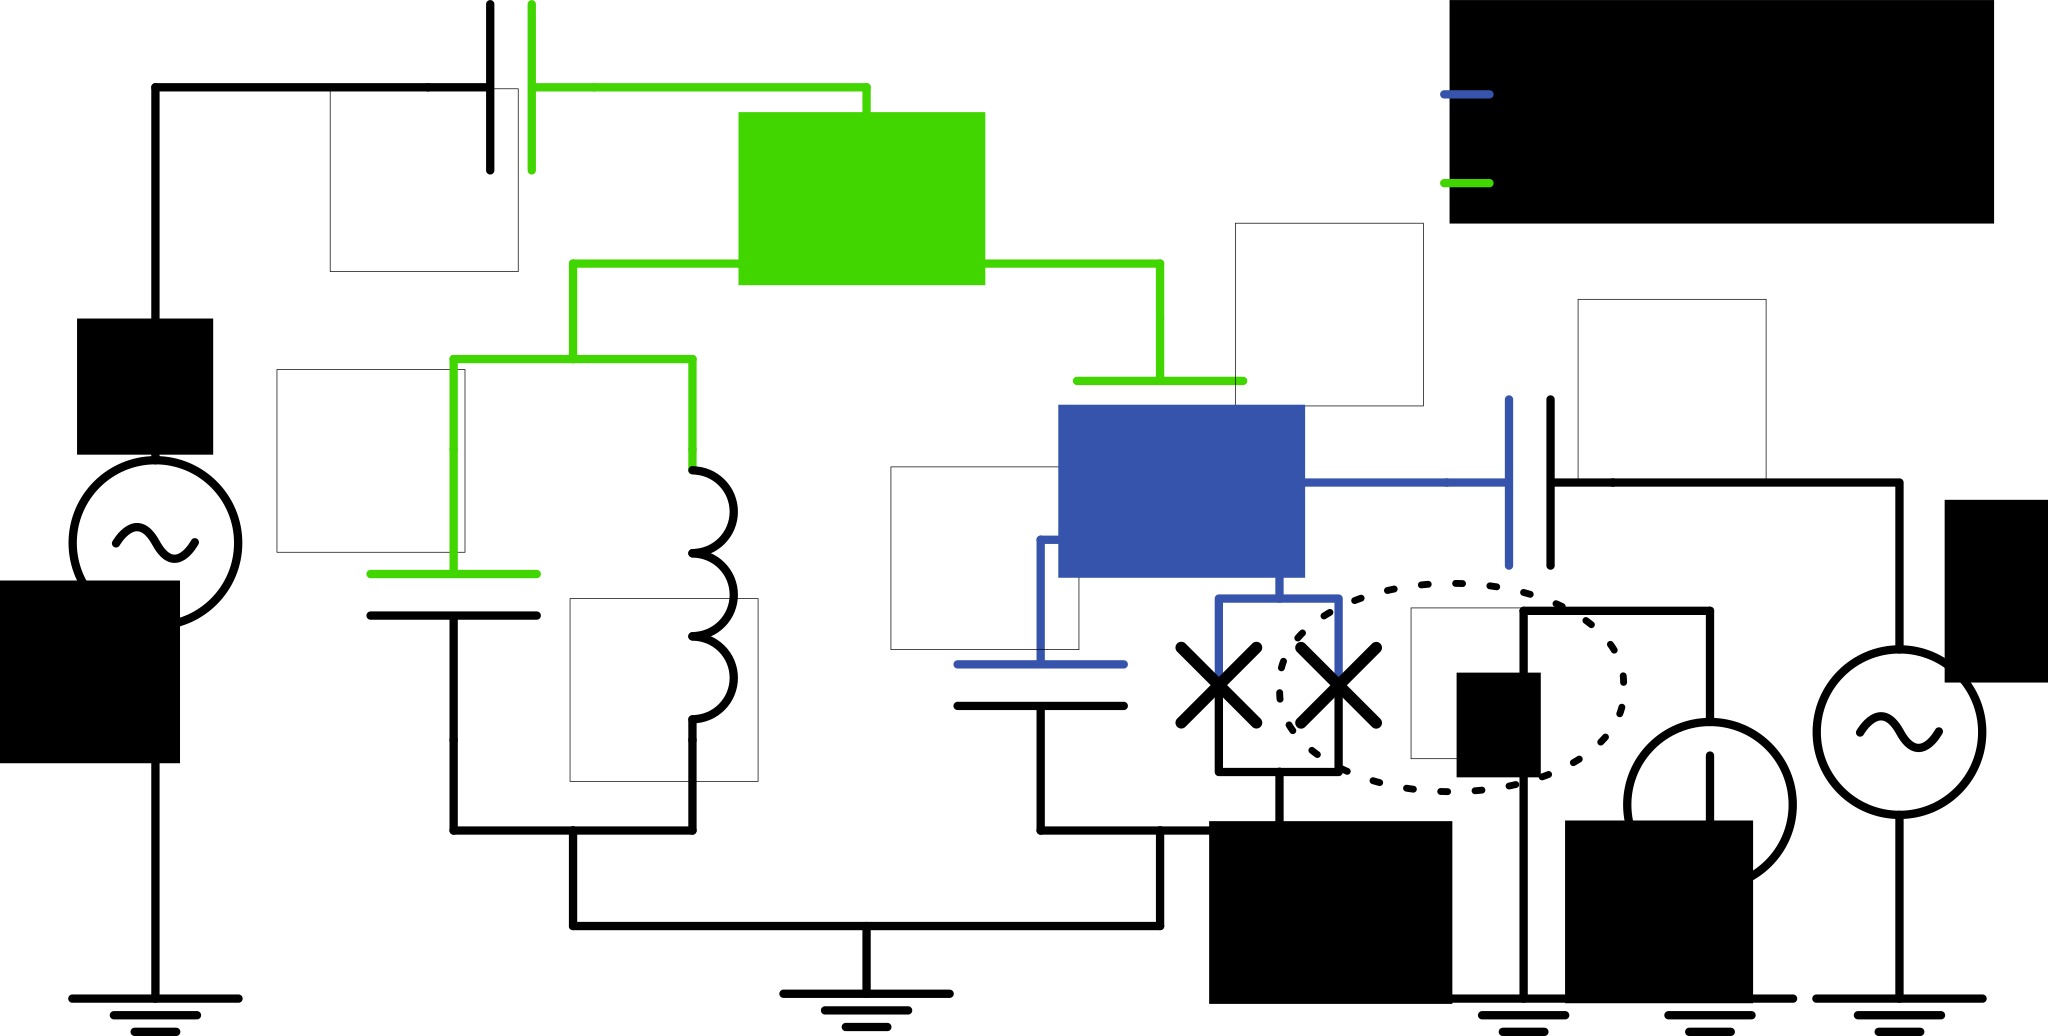
\includegraphics[width=0.8\textwidth]{xmon-resonator}
\caption{Equivalent circuit for coupled system of a tunable transmon qubit and a resonator. Colors show nodes (or branches) containing system's degrees of freedom according to M. Devoret's theory\cite{Devoret1995}.}
\label{fig:xmon-resonator}
\end{figure}

First of all, it is necessary to construct the full Hamiltonian for the transmon-oscillator system depicted in \autoref{fig:xmon-resonator}. We will use the results acquired by Bader\cite{Bader2013} and Koch\cite{Koch2007}. The system under study has two degrees of freedom; one from the resonator and one from the qubit. The coupling between the systems is achieved due to the presence of a capacitor $C_g$ whose energy depends on both degrees of freedom. The Lagrangian of the circuit is then easy to write down, and with some calculations it is possible to obtain as well the quantized Hamiltonian for the compound circuit:

\begin{equation}
\begin{gathered}
\mathcal{\hat H} =  \underbrace{\frac{\hat \phi_r^2}{2 L_r} + \frac{(C_q+C_g) \hat Q_r^2}{2C_*^2}}_\text{resonator} 
+ \underbrace{\frac{(C_g + C_\kappa + C_r) \hat Q^2_q}{2C_*^2} - E_J (\Phi_{ext}) \cos \frac{2e}{\hbar}\hat \phi_q }_\text{qubit}
+ \underbrace{\frac{C_g\hat Q_r \hat Q_q}{C_*^2}}_\text{coupling} = \\
=  \hbar\omega_r\ \hat a^\dag \hat a \otimes \mathbbm{\hat 1}_q \quad (\mathcal{\hat H}_r) \\
+ 4 E_C\ \mathbbm{\hat 1}_r \otimes \hat n^2 - \frac{E_J(\Phi_{ext})}{2}\ \mathbbm{\hat 1}_r\otimes \sum_{n=-\infty}^{+\infty} \ket{n+1}\bra{n} + \ket{n}\bra{n+1} \quad (\mathcal{\hat H}_q) \\
- 2e \frac{C_g}{C_*} \sqrt{\frac{\hbar \omega_r }{2(C_q+C_g)}}\ i(\hat a^\dag - \hat a) \otimes \hat n, \quad (\mathcal{\hat H}_i)
\end{gathered}\label{eq:hamiltonian}
\end{equation}
where 
$$C_*^2 = C_q C_g + C_q C_\kappa + C_g C_\kappa + C_q C_r + C_g C_r, $$
$$\omega_r = 1/\sqrt{L_r C_*^2/(C_q+C_g)}, $$
$$E_C = \frac{(C_g+C_\kappa+C_r)e^2}{C_*^2}, $$
$$E_J(\Phi_{ext}) = E_{J,\Sigma} \cos(\Phi_{ext}/\Phi_0),\ \Phi_{ext} = I_\Phi M.$$
Presuming the coupling is not very strong ($C_g \ll C_q, C_r$) it is possible also to include simple time-dependent driving terms for both subsystems:
\begin{gather}
\mathcal{\hat H}_r^d(t) = \frac{C_\kappa V_\kappa(t)}{C_r + C_\kappa} \hat Q_r \propto f_r(t)\ i(\hat a^\dag - \hat a) \otimes \mathbbm{\hat 1}_q, \notag \\
\mathcal{\hat H}_q^d(t) = \frac{C_e V_e(t)}{C_q + C_e} \hat Q_q \propto f_q(t)\  \mathbbm{\hat 1}_r \otimes \hat n,
\label{eq:driving_q}
\end{gather}
where $f_{q, r} (t)$ are the effective values of the drive magnitudes at time $t$.

\begin{figure}
\centering
\begin{subfigure}[t]{\textwidth}
\centering
\includegraphics[width=0.9\textwidth]{levels}
\end{subfigure}

\begin{subfigure}[t]{\textwidth}
\centering
\includegraphics[width=0.9\textwidth]{freqs}
\end{subfigure}
\caption{Energy structure and transition frequencies (from the ground state) of the transmon-resonator system depending on $\Phi_{ext}$.}
\label{fig:levels}
\end{figure}


\begin{figure}[h]
\centering
\includegraphics[height=0.25\textheight]{diagram_q>r}\ \includegraphics[height=0.25\textheight]{diagram_q<r}
\caption{Energy level diagrams for the transmon-resonator system in the sweet spot when the detuning $\Delta_\omega = \omega_r-\omega_{ge}$ is negative (right) or positive (left).}
\label{fig:diagram}
\end{figure}

\subsection{Energy spectrum of the transmon-resonator system}

Using QuTiP\cite{Johansson2011} it is easy to solve the truncated matrix eigenproblem with the Hamiltonian \eqref{eq:hamiltonian}. The results for the typical design values
$$
C_\kappa = 5 \text{ fF},\ C_g = 2 \text{ fF},\ C_q = 90 \text{ fF},\ C_r = 500 \text{ fF},\ L_r = 2 \text{ nH}, $$
$$E_{J, \Sigma} = (h \nu_q + E_C)^2/8 E_C\ \text{for\cite{Koch2007}}\ \nu_q = 6\ \text{GHz}
$$
can be observed in \autoref{fig:levels}.

In \autoref{fig:diagram} the energy structure of the compound system in the sweet-spot ($\Phi_{ext}=0$) is shown for two cases of positive and negative detuning. The dispersively shifted frequencies can be calculated from perturbation theory. For example, for the transition $\ket{0, g}\rightarrow \ket{1, g}$ the shift is defined to the second order as
\begin{align*}
\chi_0 &=  E_{1g}^{(1)} + E_{1g}^{(2)} - E_{0g}^{(1)} - E_{0g}^{(2)}\\
 &= \bra{1, g}\mathcal{\hat H}_i\ket{1,g} + \sum_{i, \alpha \neq 1, g} \frac{|\bra{g, 1}\mathcal{\hat H}_i\ket{i,\alpha} |^2}{E_{1g} - E_{i\alpha}}\\
 & - \bra{0, g}\mathcal{\hat H}_i\ket{0,g} - \sum_{i, \alpha \neq 0, g} \frac{|\bra{g, 0}\mathcal{\hat H}_i\ket{i,\alpha} |^2}{E_{1g} - E_{i\alpha}}.
\end{align*}
As long as $\mathcal{\hat H}_i$ mixes only adjacent resonator states the first order corrections vanish, and so do the summations over $i$: $\sum_{i, \alpha} \rightarrow \sum_{0,\alpha} + \sum_{2,\alpha} (\sum_{1,\alpha})$. These sums then can be further truncated:
\begin{equation}
E_{1g}^{(2)} - E_{0g}^{(2)} \approx \frac{|\bra{g,1}\mathcal{\hat H}_i\ket{0,e}|^2}{\omega_r - \omega_{ge}} + \frac{|\bra{g,1}\mathcal{\hat H}_i\ket{2,e}|^2}{\omega_r - 2\omega_r - \omega_{ge}} -
\frac{|\bra{g,0}\mathcal{\hat H}_i\ket{1,e}|^2}{-\omega_r - \omega_{ge}}\label{eq:chi0_truncsums}
\end{equation} 
due to the selection rule of $\hat n$: $\bra{E^q_n}\hat n \ket{E^q_{n+2k}} = 0,\ k \in \mathbb{Z}$ and the fast (exponential from numerics) decay of its matrix elements over distance between transmon energy eigenstates (see \autoref{sec:tr_eigen}). It can be easily proven that last two elements of \eqref{eq:chi0_truncsums} are equal up to the factor of $\sqrt{2}^2$ and final equation for $\chi_0$ follows
\begin{equation}
\chi_0 = g^2\sbrkt{\frac{n_{ge}^2}{\omega_r - \omega_{ge}}-\frac{n_{ge}^2}{\omega_r + \omega_{ge}}}.
\label{eq:chi0}
\end{equation}

\begin{figure}[h!]
\centering
\includegraphics[height=0.25\textheight]{shifts-10.pdf}
\includegraphics[height=0.25\textheight]{shifts10.pdf}
\caption{Dispersive shifts for the first three states of the transmon in dependence on the external flux. Solid lines are numerical solution and dashed lines are results from equations \eqref{eq:chi0}-\eqref{eq:chi2}.}
\label{fig:disp_shifts}
\end{figure}

Similarly, dispersive shifts for the other two transmon states are derived:
\begin{gather}
\chi_1 = g^2\sbrkt{\frac{n_{ef}^2}{\omega_r - \omega_{ef}} - \frac{n_{ef}^2}{\omega_r + \omega_{ef}} + \frac{n_{eg}^2}{\omega_r + \omega_{ge}}-\frac{n_{eg}^2}{\omega_r - \omega_{ge} }},\label{eq:chi1}
\\
\chi_2 = g^2\sbrkt{\frac{n_{fd}^2}{\omega_r - \omega_{fd}} -\frac{n_{fd}^2}{\omega_r + \omega_{fd}} + \frac{n_{fe}^2}{\omega_r + \omega_{ef}}- \frac{n_{fe}^2}{\omega_r -\omega_{ef}}},
\label{eq:chi2}
\end{gather}
where $g, e, f, d$ denote the first 4 energy eigenstates of the transmon, $n_{\alpha\beta} = \bra{\alpha} \hat n \ket{\beta}$ is the matrix element of $\hat n$ and $g = \left.|\frac{\mathcal{\hat H}_i}{i(\hat a^\dag  - \hat a)\otimes \hat n}|\right.$ is the coupling parameter which precedes the operator part in the interaction Hamiltonian. In \autoref{fig:disp_shifts} these formulas are compared to the numerical solution. As can be seen, the analytical solution is quite accurate at the detunings of about 1 GHz. Note that dispersive shift $\chi_1$ is always smaller than $\chi_0$ when the detuning is large enough meaning that the resonator frequency will move down from its initial position. There is also another regime which occurs when the resonator frequency is situated between transitions $ge$ and $ef$ and is called \textit{straddling regime} by Koch et al.\cite{Koch2007}. The dispersive regime breaks down there when the coupling is strong enough (i.e., 50 MHz) and the anharmonicity of the qubit is not very large (i.e., 200 MHz) compared to it, so the second order correction equations become inaccurate. In this regime, however, $\chi_1>\chi_0$, and the resonator moves up when the qubit is excited.


\section{Dynamics}\label{sec:dynamics}

\subsection{Driving of an isolated transmon}

To simulate the dynamics in the unitary case without taking into account the dissipative processes, it is enough to solve the Schrödinger equation with the Hamiltonian \eqref{eq:hamiltonian} summed with the driving part \eqref{eq:driving_q}. The final state after some time of the evolution $t$ will be described with a Dyson series or a $\hat T$-exponent:
\begin{equation}
\begin{aligned}
\ket{\psi (t)} &= \hat T \exp\left\{-\frac{i}{\hbar} \rbrkt{\mathcal{\hat H}_{tr}t + \int_0^t \mathcal{\hat H}_q^d(\tau) \diff\tau}\right\} \ket{\psi(0)}\\
&\equiv \hat U(t, 0) \ket{\psi(0)}\equiv \sum_k c_k(t) \ket{E^q_k},
\end{aligned}
\label{eq:dyson}
\end{equation} 
where $\ket{E_k^q}$ denotes the $k$'s eigenstate of the qubit Hamiltonian and $\hat U(t, 0)$ is the standard evolution operator. There is no exact analytical solution for $c_k(t)$ for the transmon qubit, so we will use some approximations, perturbation theory and numerical methods to get an insight into the dynamics of this quantum system.

\subsubsection{Approximate solution for two-level dynamics} \label{sec:tr_rwa}

Let's write down the matrix equation for the time-dependent Schrödinger's equation in the energy representation of the transmon:

\begin{equation*}
i\hbar \left(
\begin{matrix}
\dot c_g \\
\dot c_e\\
\dot c_f\\
\dot c_d\\
\vdots
\end{matrix}
\right) = 
\left[\left(
\begin{matrix}
E_g & 0 & 0 & 0 & \cdots\\
0 &E_e & 0 & 0 & \cdots\\
0 & 0 & E_f & 0 & \cdots\\
0 & 0 & 0 & E_d & \cdots\\
\vdots&\vdots&\vdots&\vdots& \ddots
\end{matrix}
\right)
+
f(t)
\left(
\begin{matrix}
0          & n_{ge} & 0         & n_{gd} & \cdots\\
n_{eg} & 0          & n_{ef} & 0         & \cdots\\
0          & n_{fe}  & 0         & n_{fd} & \cdots\\
n_{dg} & 0          & n_{df} & 0         & \cdots\\
\vdots&\vdots&\vdots&\vdots& \ddots
\end{matrix}
\right)\right]
\left(
\begin{matrix}
c_g\\
c_e\\
c_f\\
c_d\\
\vdots
\end{matrix}
\right).
\end{equation*}
Here we have used the properties of the $\hat n$ (see \autoref{sec:tr_eigen}) operator to simplify its matrix representation. Now we can write down the differential equations for three lowest levels:
\begin{equation}
\begin{cases}
i\hbar \dot c_g = E_g c_g + f(t) (n_{ge} c_e + n_{gd} c_d + \cdots),\\
i\hbar \dot c_e = E_e c_e + f(t) (n_{eg} c_g + n_{ef} c_f + \cdots),\\
i\hbar \dot c_f = E_f c_f + f(t) (n_{fe} c_e + n_{fd} c_d + \cdots).
\end{cases}
\label{eq:c_gef_ode}
\end{equation}
Then we use the following ansatz: $c_\alpha = c_\alpha' \exp( - i \frac{E_\alpha t}{\hbar})$, which transforms the Hamiltonian into the \textit{rotating frame} (or the \textit{interaction picture}). In this frame, the unperturbed Hamiltonian is equal to $\hat 0$, and the equations \eqref{eq:c_gef_ode} become (omitting apostrophes):

\begin{equation}
\begin{cases}
i\hbar \dot c_g =  f(t) (n_{ge} c_e e^{-i\omega_{ge}t}+ n_{gd} c_d  e^{-i\omega_{gd}t} + \cdots),\\
i\hbar \dot c_e =  f(t) (n_{eg} c_g e^{i\omega_{ge}t} + n_{ef} c_f e^{-i\omega_{ef}t}+ \cdots),\\
i\hbar \dot c_f =   f(t) (n_{fe} c_e e^{i\omega_{ef}t}+ n_{fd} c_d e^{-i\omega_{df}t} + \cdots).
\end{cases}
\label{eq:c_gef_ode_rf}
\end{equation}

Finally, assuming harmonic perturbation at $ge$ transition frequency, $f(t) = \hbar f \cos(\omega_{ge} t + \phi ) = \frac{\hbar f}{2}(e^{i\omega_{ge} t+i\phi} + e^{-i\omega_{ge} t-i\phi})$, and dropping all oscillating terms (\textit{rotating wave approximation, RWA}), we obtain the standard two-level dynamics for Rabi oscillations around the axis $\phi$ degrees away from the $x$-axis of the Bloch sphere with angular frequency of $\Omega_R = f n_{ge}$:
\begin{equation}
\begin{cases}
i\hbar \dot c_g =  \frac{\hbar fe^{i\phi}}{2} n_{ge} c_e,\\
i\hbar \dot c_e =   \frac{\hbar fe^{-i\phi}}{2} n_{eg} c_g.
\end{cases} \Leftrightarrow\  i\partial_t \ket{\psi (t)} = \frac{\Omega_R}{2}[\cos(\phi)\hat \sigma_x + \sin(\phi)\hat \sigma_y]\ket{\psi(t)}.
\label{eq:rwa_ode}
\end{equation}

\begin{figure}
\centering
\includegraphics[width=.4\textwidth]{2d_rabi_example_bloch_pure}\quad
\includegraphics[width=.4\textwidth]{2d_rabi_example_bloch_pure_Y}
\caption{Visualization of the solution of \eqref{eq:rwa_ode} on the Bloch sphere for $\Omega_R=5$ MHz and two values of $\phi$: 0 (left) and $-\pi/2$ (right).}
\label{fig:bloch_rot}
\end{figure}

The exact solution for this equation may be obtained with use of the matrix exponent and the following properties of $\hat \sigma_{x,y}$: $\hat \sigma_x^2 = \mathbbm{\hat 1},\ \hat \sigma_x^3 = \hat\sigma_x$. However, since $\hat \sigma_x$ and $\hat \sigma_y$ are not commuting, it is a bit cumbersome to calculate the matrix exponent when $\phi$ is arbitrary, and it's easier just to switch the basis so that $\phi=0$. So below we solve the equation in this case:
\begin{equation}
\begin{aligned}
\ket{\psi(t)} &= \exp\{i\frac{\Omega_R}{2}\hat \sigma_x t\} \ket{\psi(0)}\\
& = \left[\mathbbm{\hat 1} \cos\left(\frac{\Omega_R}{2}  t\right) + i\hat \sigma_x \sin\left(\frac{\Omega_R}{2} t\right)\right]\ket{\psi(0)}. 
\end{aligned}
\end{equation}
With initial state $\ket{g}$, we can calculate the probability of being in the states $\ket{e}$ and $\ket{+} = \frac{1}{\sqrt{2}}(\ket{g}+\ket{e})$ to be  as follows:
\begin{equation}
\begin{aligned}
P(\ket{e})(t) &= |\braket{e}{\psi(t)}|^2 = \frac{1-\cos(\Omega_R t)}{2},\\
P(\ket{+})(t) &= |\braket{+}{\psi(t)}|^2 = \frac{1}{2}.
\end{aligned}
\label{eq:x_rotation}
\end{equation}
Clearly, this is by definition the rotation around the $x$-axis. The $y$ rotation may be derived in a similar way if the phase is chosen to be $\pi/2$. 

In general, using these formulas, we can define $(\theta)^{x(y)}$-pulse as windowed sine wave with window of correct amplitude, duration and phase, so that the qubit is rotated $\theta$ radians around the corresponding axis (see \autoref{fig:bloch_rot}). For example, for a fixed-length pulse of $t_g$, the $(-\frac{\pi}{2})^{y}$-pulse amplitude $f_q$ should be $- \pi/2 t_g n_{ge}$ and pulse phase $\phi$ equal to $-\pi/2$. Conversely, for a fixed $\Omega_R$ (drive amplitude $f_q$) to perform the same rotation the pulse time $t_g$ should be chosen as $\pi/2\Omega_R$ for the excitation signal with the phase increased by $\pi$ (as $t_g\geq 0$).

\subsubsection{Time-dependent perturbation theory}

Perturbation theory allows semianalytical calculation of the transition rates	(Rabi oscillation frequencies) for single and multi-photon processes. Using the the Dyson series we can write down the expansion of the evolution operator $\hat U(t, t_0)$  and then use it to calculate the expansion of the transition rate $A_{fi} = \bra{f}\hat U(t, t_0)\ket{i}$ from some initial state $\ket{i}$ to the final state $\ket{f}$ under some driving operator $\hat V(t)$. Here is the result for the $\hat U(t, t_0)$ decomposition:\cite{faisal2013}
\begin{equation}
\begin{aligned}
\hat U(t, t_0) &= 1 + \sum_n \hat U^{(n)}(t, t_0),\\
\hat U^{(n)}(t, t_0) &= \left(-\frac{i}{\hbar}\right)^n\int\limits_{t_0}^t \diff t_1 \hat V_I(t_1)\int\limits_{t_0}^{t_1} \diff t_2 \hat V_I(t_2)\cdots\int\limits_{t_0}^{t_{n-1}} \diff t_n \hat V_I(t_n),
\end{aligned}
\end{equation}
where $\hat V_I(t) = \exp(i\mathcal{\hat H}_{tr}(t-t_0)/\hbar) \hat V(t) \exp(-i\mathcal{\hat H}_{tr}(t-t_0)/\hbar)$ is the driving operator in the interaction picture (same as in the rotating frame). For example, let's reproduce the previous result and calculate the Rabi frequency for the single-photon transition.  The transition rate $A^{(1)}_{eg}(t) = \bra{e}\hat U^{(1)}(t, t_0)\ket{g}$ when $\hat V(t) = \hbar f \hat n \cos(\omega t)$ is calculated as follows :
\begin{equation}
A^{(1)}_{eg}(t) = - i \frac{f n_{eg}}{2} \int\limits_{t_0}^t e^{i\omega_{ge} t_1} (e^{i\omega t_1}+e^{-i\omega t_1})\diff t_1.
\end{equation}
In the limit of ${t-t_0\gg1/\omega}$ and $\omega - \omega_{ge}\ll1$ this can be rewritten as
\[
A^{(1)}_{eg}(t) \sim - i \frac{f n_{eg}}{2} t.
\]
Consequently, $P(\ket{e}) = |A_{eg}|^2 = (f n_{eg}/2)^2t^2$, and this is exactly the first term of the expansion of the first formula in \eqref{eq:x_rotation} thus giving us the same Rabi frequency of $f n_{eg}$. 

Multi-photon transition rates are harder to calculate since they require summations over different intermediate states $\ket{j}$ between the initial and the final state. Nevertheless, below we will calculate the Rabi frequency of the two-photon $gf/2$ transition, so that $\omega \approx \omega_{gf}/2$. The first order correction vanishes for this transition, and thus we need to calculate the second order correction only. Following Faisal\cite{faisal2013}, we obtain:
\[
A^{(2)}_{fg}(t) \sim  i (f/2)^2 \sum_j \frac{n_{fj}n_{jg}}{\omega_{gj}-\omega_{gf}/2} t \approx  i (f/2)^2 \frac{n_{fe}n_{eg}}{\omega_{ge}-\omega_{gf}/2} t.
\]
Analogously to the previous case, this gives us the two-photon Rabi frequency: 
\begin{equation}
\Omega_{R, gf}^{2p} = \frac{f^2  n_{fe}n_{eg}}{|\alpha|} ,
\label{eq:rabi_2p}
\end{equation}
where $\alpha$ is the anharmonicity of the transmon. Note that it is proportional to the squared drive strength -- a standard result for a 2-photon process. This formula will be tested numerically in the section below.
 
\begin{figure}[h!]
\centering
\includegraphics[width=0.32\textwidth]{tr_10.0MHz_dr}
\includegraphics[width=0.32\textwidth]{tr_100.0MHz_dr}
\includegraphics[width=0.32\textwidth]{tr_200.0MHz_dr}
\caption{Dynamics of the isolated driven transmon qubit with different drive strengths $f_q/2\pi$ = 0.01-0.2 GHz, where $f_q$ is an effective amplitude of the drive \eqref{eq:driving_q} $f_q (t) = \hbar  f_q \cos(\omega_{ge} t)$. It can be seen that significant distortions and leakage to higher levels occur when amplitude becomes comparable to the transmon's anharmonicity.}
\label{fig:driven_tr}
\end{figure}

\begin{figure}[h!]
\centering
\includegraphics[height=0.185\textheight]{tr_xyz10}\includegraphics[height=0.185\textheight]{tr_xyz20}\includegraphics[height=0.185\textheight]{tr_xyz50}
\caption{Numerical solution for the two-level behaviour of the transmon in the computational basis for different drive strengths. Note the phase error due to the leakage to the higher levels which is growing with the driving strength and is noticeable even when the drive strength is small compared to the anharmonicity.}
\label{fig:xyz_tr}
\end{figure}

\subsubsection{Numerical solution for two-level dynamics}

The simulation of the transmon dynamics can be performed as a standard numerical linear ODE solution which is also possible within QuTiP framework using the \textit{mesolve} routine. Below the results for the following model will be presented:
\[
\mathcal{\hat H} = \mathcal{\hat H}_{tr}  +\mathcal{\hat H}_q^d(t),\ f_q^d(t) =\hbar f_q \cos(\omega_{ge}t),\ \omega_{ge}/2\pi = 6\ \text{GHz},\ \alpha/2\pi = - 200\ \text{MHz}.
\]
We can solve the time-dependent Schrödinger equation with this Hamiltonian with $\ket{g}$ as the initial state to obtain system state $\ket{\psi(t)}$ as each time point we need, and then calculate the projections of these states onto the eigenstates to find decomposition coefficients $c_{g}..c_{d}$. Alternatively, it is possible to  find the expectation values for the quasi-two-level operators
\[
\hat \sigma_x = \ket{g}\bra{e}+\ket{e}\bra{g},\ \hat\sigma_y = i\ket{g}\bra{e} - i\ket{e}\bra{g},\ \hat\sigma_z  = \ket{e}\bra{e}-\ket{g}\bra{g}
\]
for each state $\ket{\psi(t)}$ which allow us to find its phase in the \textit{computational basis}. However, when higher levels are involved in the dynamics, these expectation values loose their meaning and should be used with discretion.

The result of such simulations can be observed in \autoref{fig:driven_tr} and \autoref{fig:xyz_tr}. As one can see, when the driving amplitude becomes comparable to the anharmonicity of the transmon, significant leakage to higher states occurs which in the computational basis manifests itself as a phase error. This error is significant even when the driving strength is relatively small, so special techniques such as Derivative Removal by Adiabatic Gate\cite{Motzoi2009,Chow2010} (DRAG) or Half Derivative\cite{Lucero2010} (HD) method were suggested to cope with it.

DRAG procedure can correct any continuous pulse rotating the qubit around some axis (i.e., $(\pi)^x$) by adding two simultaneous pulses around two other axes. If the  $(\pi)^x$-pulse has the windowing function $F_x(t)$, the pulses around $y$-axis and $z$-axis (which is usually just a DC-pulse, i.e., pulse with no carrier, providing dynamic detuning of the qubit during this operation) should be constructed as follows:
\[
F_y = -\frac{\dot F_x}{\alpha},\ \omega-\omega_{ge}(t) = \frac{(\lambda^2-4)F_x^2}{4\alpha}
\]
However, it is possible to alleviate the necessity of $z$-pulses by putting $F_y=-\frac{1}{2}\frac{\dot F_x}{\alpha}$. This change significantly reduces the complexity of the original DRAG operation while maintaining approximately the same performance, as numerical simulations has shown\cite{Lucero2010}. The resulting operation is named the Half Derivative method after the factor of 1/2 before $\dot F_x$, and not because it is somehow connected to fractional calculus.

\begin{figure}
\centering
\includegraphics[width=0.32\textwidth]{tr_2p_1MHz_dr} \includegraphics[width=0.32\textwidth]{tr_2p_5MHz_dr} \includegraphics[width=0.32\textwidth]{tr_2p_10MHz_dr}
\caption{Simulated two-photon $gf/2$ Rabi oscillations. The Rabi frequency is closer to the theoretically predicted one in \eqref{eq:rabi_2p} when the drive is weak and deviates more and more when the drive strength is increased. Higher-frequency oscillations are present, too, and also grow with the drive amplitude.}
\label{fig:2p_sim}
\end{figure}

\subsubsection{Numerical solution for two-photon dynamics}

Similarly to the single-photon two-level process simulated above, we can simulate the two-photon transition $gf/2$. To test the equation \eqref{eq:rabi_2p}, we put $f_q$ which is the amplitude of the two-photon driving $f_q \cos(\omega_{fg}/2+t)$ to be as follows:
\[
f_q = \sqrt{\frac{\Omega_{R,gf}^{2p} |\alpha|}{n_{ge}n_{ef}}},
\]
where $\Omega_{R,gf}^{2p}$ is the two-photon Rabi frequency which we want to observe. The results of the numerical simulation performed with this method are presented in \autoref{fig:2p_sim}. For $\Omega_{R,gf}^{2p}/2\pi =$ 1 MHz (5 MHz, 10 MHz), we observe the two-photon Rabi frequency of 1.03 MHz (5.2 MHz, 11 MHz) which is a good match considering the perturbative nature of the the equation \eqref{eq:rabi_2p}. 

\begin{figure}
\includegraphics[width=.5\textwidth]{tr_decay}\hspace{-7.5cm}\textbf{(a)}\hspace{6.5cm}
\includegraphics[width=.5\textwidth]{tr_str_dr_decay}\hspace{-7.5cm}\textbf{(b)}\hspace{6.5cm}
\caption{Behaviour of the equation \eqref{eq:tr_dissip_dyn}, represented as populations of the eigenstates depending on time. \textbf{(a)} Relaxation of the first excited state without any driving. The population reaches $1/e$ in $1/\gamma$ ns, as expected. \textbf{(b)} Excitation of the ground state into the steady state which is an incoherent mixture of the first three states. Driving is resonant with the $ge$ transition of the transmon.}
\end{figure}

\subsection{Relaxation dynamics (driven and undriven)}

The relaxation process for the transmon is simulated using a Lindbladian master equation with a following dissipative operator:
\begin{equation}
\hat c = \sum_{j\geq 0}^\infty \frac{n_{j\,j+1} }{n_{01}}\ket{j}\bra{j+1}
\end{equation}
which is from the definition a lowering operator. It becomes the annihilation operator of the standard harmonic oscillator in the limit of very large $E_J/E_C$, so it is a good operator to model the relaxation channel. For a deeper review on this, see L.S. Bishop's PhD thesis.\cite{Bishop2010}

The dynamics of the dissipative transmon then will be governed by the following equation:
\begin{equation}
\frac{\partial}{\partial t} \hat{\rho}_q = \frac{i}{\hbar}[\hat{\rho}_q, \hat{\mathcal{H}}_q+\hat{\mathcal{H}}_q^d(t)] + \gamma \mathcal{D}[\hat c]\hat\rho_q,
\label{eq:tr_dissip_dyn}
\end{equation}
where $ \mathcal{D}[\hat{\mathcal{O}}]\hat\rho_q = \hat{\mathcal{O}} \hat\rho_q \hat{\mathcal{O}}^\dag - \frac{1}{2}\{\hat{\mathcal{O}}^\dag \hat{\mathcal{O}}, \hat\rho_q \}$ and $\gamma$ is the relaxation rate. Pure dephasing may also be added in a similar way.

Below the dynamics of the undriven relaxation and excitation with strong driving are presented as examples of the solution of \eqref{eq:tr_dissip_dyn}.

\subsection{Linewidth dependence on drive power} \label{subsec:linewidth}

\subsubsection{Two-level model}

Knowing the way to model the relaxation of the qubit, it is possible to compare the relaxation rate with the linewidth of the qubit on the population graph. The way is to simulate the evolution until the steady state is reached for all driving frequencies around the resonance, calculate populations of the excited state for each reached steady state and then measure the width at the half-maximum of the resulting peak. However, for two-level dynamics the linewidth $\delta \omega$ depends on the driving power as the Rabi oscillations are induced between the levels. So for correct determination of the linewidth it's necessary to measure the linewidth at low driving amplitudes.

Before demonstrating the numerical results for the transmon qubit, a brief analytical solution for the problem in the case of a two-level system will be shown. The master equation for this problem is as follows (within the RWA):
\[
\frac{\partial}{\partial t} \hat{\rho}_{tls} = \frac{i}{\hbar}[\hat{\rho}_{tls}, \frac{\hbar (\overbrace{\omega_{tls}-\omega_d}^{\Delta\omega})}{2} \hat{\sigma}_z+\frac{\hbar \Omega_R}{2} \hat{\sigma}_x] + \gamma \mathcal{D}[\hat \sigma^-]\hat\rho_{tls}.
\]
Knowing that $\text{Tr}[\hat\rho_{tls}]=1$ and that $\hat\rho_{tls}=\hat\rho_{tls}^\dag$ we can write down three ODEs from this master equation:
\[
\begin{gathered}
\frac{d}{d t} {ρ_{11}}{\left (t \right )} = - γ {ρ_{11}}{\left (t \right )} + i \left(\frac{Ω_{R}}{2} {ρ_{12}}{\left (t \right )} - \frac{Ω_{R}}{2} {ρ_{21}}{\left (t \right )}\right), \\
\frac{d}{d t} {ρ_{12}}{\left (t \right )} = - \frac{γ}{2} {ρ_{12}}{\left (t \right )} + i \left( \frac{Ω_{R}}{2} {ρ_{11}}{\left (t \right )} - \frac{Ω_{R}}{2} \left(1- {ρ_{11}}{\left (t \right )} \right) - \Delta ω {ρ_{12}}{\left (t \right )}\right),\\
{ρ_{21}}{\left (t \right )} = {ρ_{12}}^\dag{\left (t \right )}.
\end{gathered}
\]

It is practical for our case to solve these equations for the \textit{steady state}, when $\frac{\partial}{\partial t} \hat{\rho}_{tls} = 0$. The matrix elements then are
\[
ρ_{11} = \frac{Ω_{R}^{2}}{2 Ω_{R}^{2} + γ^{2} + 4 \Delta ω^{2}},\quad
ρ_{12} = - \frac{Ω_{R} \left(i γ + 2 \Delta ω\right)}{2 Ω_{R}^{2} + γ^{2} + 4 \Delta ω^{2}},\quad
ρ_{21} = \frac{Ω_{R} \left(i γ - 2 \Delta ω\right)}{2 Ω_{R}^{2} + γ^{2} + 4 \Delta ω^{2}}.
\]

From here it is easy to find the analytical linewidth at half maximum of the $\rho_{11}(\omega_d)$:
\[
\delta\omega = \sqrt{2\Omega_R^2+\gamma^2}.
\]

When the $\Omega_R \rightarrow 0,\ \delta\omega\rightarrow\gamma$, and thus it is possible to extract $T_1$ in case of absence of pure dephasing, or at least to put a lower bound on it if pure dephasing is present. It is important to notice that in the experiment the measured frequency is expressed in Hz though $\delta\omega$ is in rad/s. Therefore, the experimental linewidth should be, firstly, measured at very low powers and, secondly, multiplied by $2\pi$ to obtain $\gamma$. In the presence of pure dephasing the formula for $\delta\omega$ becomes a bit more complicated, but also can be straightforwardly calculated with use of Computer Algebra Systems:
\[
\delta\omega_{\text{with dephasing}} = \sqrt{2Ω_{R}^{2} (1+2 γ_{ϕ}/\gamma) + (\gamma +2\gamma_\phi)^2} \xrightarrow[\Omega_R\rightarrow 0]{} γ + 2γ_{ϕ}.
\]

Interestingly enough, if there's no relaxation and $\gamma = 0$, the formula shows divergence of the linewidth. This happens because the solution of the master equation in this case yields $\rho_{11} = 1/2$ in the steady state, independent of the driving detuning and driving strength, and thus the linewidth can not at all be defined.


\begin{figure}
\centering
\includegraphics[width=\textwidth]{transmon_transtitions_narroww_gamma5e-3}

\includegraphics[width=0.7\textwidth]{linewidth_prop_ss}
\caption{Linewidth analysis in dependence on the driving power $f_q$ for $\gamma = 5$ rad/$\mu$s. As can be seen, with the increasing drive amplitude the spectral line becomes wider. In contrast, its width levels off when the amplitude is decreased, and reaches asymptotically the value of $\frac{\gamma}{2\pi}$. The factor $2\pi$ appears as long as the linewidth found in the experiment usually is in Hz, but the equality that holds is that $\gamma = \delta\omega$, and $\delta\omega = 2\pi\delta\nu$.}
\label{fig:transmon_lw}
\end{figure}  
\subsubsection{Transmon case}

For the transmon, the two-level dynamics between its ground and first excited state is equivalent; however, there's no simple analytical solution for the dynamics between many levels. To see the behaviour is the same in this case we have to resort to numerical modelling (see \autoref{fig:transmon_lw}). As can be seen, the linewidth $\delta\omega$ grows with the increased power, and, in contrast, saturates at low powers, reaching the value of $\gamma$. The growth is exponential meaning that the linewidth is indeed proportional to the Rabi frequency similarly as what the two-level model predicts. This is expected as long as the lowering operator $\hat c$ in the computational basis is exactly equal to $\hat \sigma^-$, and, as long as the system stays inside this basis, the dynamics is completely equivalent to the one predicted by the two-level master equation. 

In contrast, when the drive strength is increased beyond the anarmonicity of the transmon, we observe clear deviations from the two-level behaviour. The numerical simulations and experimental data show that additional multi-photon transitions begin to arise, and, besides the spectral line $ge$ we have seen in \autoref{fig:transmon_lw}, we will observe several other lines appearing at higher drive amplitudes. The resulting spectrum is presented in  

\begin{figure}
\centering
\includegraphics[width=\textwidth]{transmon_transtitions}
\caption{Different single- and multi-photon transitions in a transmon predicted by the full numerical model with relaxation. The parameters are the same as in the previous simulations.}
\label{fig:transmon_transitions}
\end{figure}


%\chapter{Methods}

In this chapter we will discuss the methods and equipment that were used to engineer the samples and perform the experiments presented in the following chapter. During my Master's course, the main activities that I was undertaking were (in the chronological order):
\begin{itemize}
\item designing chips for investigating Q-factors of superconducting CPW resonators
\item designing chips with cQED systems based on transmons
\item improving experimental setup at RQC (design of PCBs, extending fridge capacity, developing software)
\item studying the Q-factors of resonators made of different superconductors
\item spectroscopy of the cQED samples
\item building a time-domain setup for XY-control and dispersive readout of a single qubit
\item time-resolved measurements
\end{itemize}  

Most of the spectroscopy was done at Institute of Solid State Physics in the Russian Quantum Center (RQC) lab and the time-resolved experiments were performed in the Artificial Quantum Systems Lab at Moscow Institute of Physics and Technology. Therefore, the setups in these two places will be used to illustrate the corresponding type of the experiment. 

First of all, some words about EM-simulations and the process of the chip design will be said, concerning both qubits and resonators. Then, the resonator measurement technique will be shown. Finally, we will turn to the qubit measurements, firstly, showing the spectroscopic part and, secondly, elaborating on the time-resolved techniques.

\section{Engineering of the samples}

\subsection{Designing CPW resonators}

\begin{figure}[t]
\includegraphics[width=\textwidth]{resonators_design_perspective}
\caption{Design perspective for the resonator samples that were studied. All resonators had the center strip width of 7 $\mu$m and the coplanar gaps of 4 $\mu$m. \textbf{(a)} Initial design, 10$\times$5 mm$^2$. Six resonators are located near the feedline, with and without an IDC at the open end (used to couple to the transmons in cQED). The asymmetric contact pad configuration was chosen to be compatible to the PCBs which were available at that moment. Resonant frequencies were non-uniformly distributed from 6 to 8.6 GHz. External quality factors were calculated to be around 6000 based on simulated transmission data. \textbf{(b)} Second version of the design. The main differences are the doubled number of the resonators on the chip (to gather more accurate statistical data) and the $Q_e$ increased up to $10^{5}$ (to facilitate the extraction of the $Q_i$ for the fitting algorithm). The frequencies were uniformly distributed from 6 to 8.2 GHz. Also, a border to simplify cutting the chips out of the waver and an ID-label to help distinguish between the samples were added. \textbf{(c)} Third iteration of the design with 24 resonators. Parameters are the same as for the second version, but the size was increased, and the contact pads adapted to the 10$\times$10 mm$^2$ PCBs.}
\label{fig:resonators_design_perspective}
\end{figure}

The CPW resonators that I wanted to use are the $\lambda/4$-type ones, coupled to the feedline as shunts (notch-type). During the 2 years of my work, I have gone through just three design versions for the samples with almost no change for the geometries of the individual resonators. This is very important: we were studying the influence of the fabrication process on the quality factors, and thus to have consistent results between different samples and to have the right to compare them one with other, at least their in-plane geometries had to be identical. The designs that were used are presented in \autoref{fig:resonators_design_perspective} in the chronological order. 

The first design, despite its simplicity, included a lot of work and formed a foundation for the future developments. It was already extensively simulated, allowed to test experimentally the semi-analytic formula\cite{Sank2014} that estimates the ``claw''-coupler influence on the resonance frequency, to test the simulated coupling Q-factors, etc. However, the main feature behind it, which was at that time a breakthrough for me and our group in Russia, was that no hand-drawing at all had been involved in its creation. In contrast, the layout was fully parametrized and programmed using the macro API of the \textit{LayoutEditor} EDA software. This technique of coding the design, though tedious in the beginning, allows in the long run to make such complex changes to the scheme which otherwise would require redrawing everything from scratch. Moreover, the algorithm, once done correctly and debugged, will make no mistakes which are inevitable when the blueprints are modified by hand. Finally, the basic structures and boolean strategies between layers that were implemented to create that first chip are still being reused and extended by me and other people in the group, which means no extra unnecessary work is done. I would like to thank Jürgen Lisenfeld from Karlsruhe Institute of Technology for showing me this method and saving days of my life from being wasted on redrawing and checking designs for errors after any change.

The  second design was mostly the same as the first one to ensure consistency between the experiments. It was embellished with a border of width equal to the half thickness of the diamond saw blade (50 microns) to facilitate dicing of the wafers and a label with a unique identifier for each sample. The external quality factors were increased up to $\approx 10^{5}$ for the resonators in this design by moving them further away from the feedline. This helps to find the internal Q-factors more accurately since the fitting algorithm, which will be described in more detail in \autoref{sec:circlefit}, finds $Q_e$ and $Q_l$ from the data, and then calculates the remaining factor from these two values (recall equation \eqref{eq:qfactor} from chapter 1). If the internal Q-factor is much higher than the external one, then $Q_e$ and $Q_i$ are nearly the same, and the error for the $Q_i$ may become large. To avoid such situations, $Q_e$ was made comparable to the highest measured $Q_i$. The number of the resonators was increased to 12 to increase the statistical sample and to be more confident in the obtained results.

The third design was filled with 24 resonators to increase the statistical accuracy even more. Otherwise, it was quite the same as the previous one.

\subsection{Simulation of CPW resonator response}

\begin{figure}[t]
\centering
\includegraphics[height=0.4\textheight]{sim_res_S21}\quad \includegraphics[height=0.4\textheight]{res_response}
\caption{Simulated $S_{21}(f)$ (left) and electrical in-plane current density near resonance (right) for an example design. The modelling was done in \textit{Sonnet Suite} 2.5D FEM software designed especially for simulating such planar structures. By fitting the parametrically plotted curve $S_{21}(f)$ in the complex plane, which is ideally a circle, the frequency and the Q-factors of the resonance may be extracted.}
\label{fig:sim_res_s21}
\end{figure}

Having the design, it is possible to directly import it into the EM-simulation software. \textit{Ansoft HFSS} is usually used for full 3-dimensional analysis, though for S-parameter computation a 2.5D-solver \textit{Sonnet Suite} is usually enough. The Sonnet simulation engine \textit{em} models the 2D structure as follows: first, it places it between two dielectric layers of given thickness and relative permittivities $\varepsilon_{1,2}$; then, this 3-layer structure is placed inside a grounded rectangular box made of perfect electric conductor. The sought S-parameters are selected by placing \textit{ports} between the ground and the electrode on which we want to set or measure the voltage. Finally, by solving the Maxwell equations in frequency domain, the voltages across the ports are found. 

Typical results for such simulation cab be observed in \autoref{fig:sim_res_s21}. The complex $S_{21}$ parameter is calculated for the ports at the feedline for each frequency. To find a single resonator response in the vicinity of its resonance frequency, Sonnet adaptive solver usually needs three frequencies at which it performs the full solution. Then it interpolates the S-parameters for the resting points and yields smooth curves which can be fitted to find the properties of the resonator under study. This interpolation is rather accurate, and thus it is practical to put a larger number of points to be interpolated so that extraction of the parameters may be done after a single run without the need of several zoom-in simulations.

Another observation for the Sonnet solver is that it gives a noticeably non-circular but rather flattened elliptical response on the complex plane around the resonant frequency when the loss is introduced into the dielectric layers; it produces a non-ideally circular response when there is no loss at all, too. That means it is not possible to find the internal Q-factor by fitting the simulation data, since it is defined exactly by the area that loses its shape. It is not clear why this is the case, as long as in the experiment the curves show such flattening only when non-linear effects come to play.\cite{astafiev2010}

The EM-simulations are quite heavy when large curved structures are considered. To perform a simulation like one shown in \autoref{fig:sim_res_s21} in an hour, it takes several gigabytes of RAM and two Intel Xeon E5-2670 processors. This computational complexity has led to development of different analytic models for estimating the external Q-factors and coupling capacitances of such structures\cite{martinis2014}; however, these methods are not simple to implement in practice and also are not very accurate. Therefore, in my work the main reference that I used was simulation data.

\subsection{Calculating transmon parameters}

\subsubsection{Capacitances}

For the transmons that were used in the experimental part of this work the only calculated parameters were the island capacitance to the ground and the coupling capacitance between the island and the open end of the resonator. These values were calculated using Sonnet by putting an autogrounded port on the qubit island and a usual port on the resonator central strip. 

\begin{figure}
\centering
\begin{minipage}{0.45\textwidth}
\includegraphics[height=0.4\textheight]{xmon_cap+g}
\end{minipage}\quad
\begin{minipage}{0.45\textwidth}
\includegraphics[height=0.35\textheight]{xmon_cap_mipt_re}

\vspace*{0.5cm}
\end{minipage}
\caption{Capacitances of the transmon island to the ground and between the island and the resonator in dependence on frequency extracted from the admittance parameters $Y_{11}$ and $Y_{21}$ (left) and in-plane current density calculated by Sonnet solver for this structure.}
\label{fig:xmon_cap}
\end{figure}

It is important that Sonnet uses the following formulas to calculate the capacitances (assuming the PI-model) from the Y-matrix:
\begin{itemize}[topsep=0pt, noitemsep]
\item from the reflection admittance $Y_{11}$: $C = -(\omega \mathfrak{Im}[1/Y_{11}])^{-1}$
\item from the transmission admittance $Y_{21}$: $C = (\omega \mathfrak{Im}[1/Y_{21}])^{-1}$
\end{itemize}
This means that if, for example, the connection between two ports is inductive or if a single port is connected to a polygon going into the ground, Sonnet will blindly follow these expressions and show negative capacitances. However, sometimes negative capacitances appear even in a correctly designed simulation after the \textit{de-embedding} process that affects interpolation; thus, only the directly calculated frequencies should be taken into account. Finally, negative capacitances sometimes appear for no clear reason and only can be overcome by changing the design parameters.

In \autoref{fig:xmon_cap} the results obtained from a two-port simulations are presented. The self-capacitance of the transmon's island and the coupling capacitance to the resonator end is calculated in a single run by looking at $Y_{11}$ and  $Y_{21}$. One can notice that their values grow with frequency; Sonnet manual explains this effect by increasing fringing fields between the fingers. However, I couldn't find any rigorous description of this effect and, since the increase is quite small, I don't take it into further calculations.

\subsubsection{Josephson junctions}

To achieve the desired $ge$ transition frequency it is not sufficient to calculate only the capacitance of the transmon's island. Recalling equation \eqref{eq:tr_levels} from Chapter 1, we see that Josephson energy $I_c h/2e$ is no less important. In practice, only the critical current is required for making the design. Usually, the calibration curve which links the oxidation exposure of the JJs with the critical current density $j_c$ is known, so it's sufficient to choose a point with a definite $j_c$ and then just calculate the required area of the junctions.

In drawing the junctions for a Dolan-bridge\cite{dolan1977} mask, two things about the geometry are important:
\begin{itemize}[topsep=0pt, noitemsep]
\item the bridge should be around 100 nm wide and around 200 nm long so that it won't sag 
\item structures near the bridge should not be very large due to the proximity effect of the electron beam
\end{itemize}

The evaporation angle needed for two layers of the junctions to overlap correctly can be found using the following formula:

\[
\zeta = \frac{180}{\pi}\arctan\rbrkt{\frac{W+w}{2H+h}},
\]
where $W$ is the width of the thinnest electrode, $w$ is the width of the bridge, $H$ is the height of the co-polymer (lower layer of the mask, $\approx$ 700 nm) and $H$ is the resist thickness (upper layer, $\approx$100 nm). In our established processes, the evaporation angle was rarely above 15 degrees, and this fact also was putting some constraints on the geometry.


\section{Extraction of resonator parameters from its scattering data}\label{sec:circlefit}

In practice, we never observe ideal circular curve on the complex plane when measuring the resonator response. This is caused by environmental contributions which are inevitably present. Such contributions are phase delay due to the length of the wiring that connects the measuring apparatus to the sample, the ideal 50-Ohm symmetric ports are replaced via wirebods of unknown impedance, the total attenuation and amplification before and after the sample is not known exactly. However, according to a paper by S. Probst et al\cite{probst2015}., these contributions may be estimated and ruled out as individual factors in a common formula. Therefore, the frequency response of a notch-type resonator as the $S_{21}$ parameter can be described with a simple formula:
\begin{equation}
S_{21}^{notch}(f) = \underbrace{ae^{i\alpha}e^{2\pi if\tau}}_\text{wiring and amplification} \underbrace{\left[1-\frac{Q_l/Q_e'}{1+2iQ_l(f/f_r-1)}\right]}_\text{mismatched resonator},
\label{eq:res_S21_probst}
\end{equation} 
where $a$ is the total amplification, $\alpha$ is the constant phase offset, $\tau$ is the time that electromagnetic wave needs to traverse the connecting cables (also called electrical or phase delay, approximately equal to 50 ns for a typical dilution fridge setup), $Q_l$ is the loaded Q-factor and $f_r$ is the resonance frequency. Finally, $Q_e'$ is the complex external quality factor. It appears to be complex in the observed $S_{21}(f)$ curve due to the impedance mismatch between the resonator ports\cite{Khalil2012} or due to the standing waves between the wirebonds\cite{Deng2013} (these explanations come from two different models, but the second model is more general). It was also demonstrated that internal quality factor can be extracted from $Q_e'$ and $Q_l$ as follows (\textit{diameter correction method, DCM}):
\[
Q_{i, \text{DCM}}^{-1} = Q_l^{-1} - \mathfrak{Re}[Q'_e]^{-1} .
\]
To sum up, using the formula \eqref{eq:res_S21_probst} to fit the experimental data, we extract all interesting parameters of the resonator. The fitting and the extraction procedure was also conveniently implemented by the author of the paper in a tool called \textit{circlefit} (it is open source and can be found on GitHub \href{https://github.com/sebastianprobst/resonator_tools/tree/master/resonator_tools}{\footnotesize{\faExternalLink}}).


\section{Experimental techniques}

In this section we will discuss hardware and methods that have been used in this work. However, since such discussions are very common in our domain and can be easily found elsewhere, only selected topics will be listed here. 

\subsection{Fridge, wiring and attenuation}

Experiments with superconducting structures working in the quantum regime require cooling of the samples down to the temperatures which ensure low populations of their excited states. Since Josephson junctions of our samples are made of Aluminium, which has a superconducting gap of 80 GHz, and since the microwave equipment (such as low-noise amplifiers) that works under $\approx$15 GHz is cheap, the usual transition frequencies between the ground and the excited states in superconducting qubits are usually close to 10 GHz. This is the reason why the dilution fridges with base temperatures from 10 to 40 mK are used everywhere in the world. I have been working with BlueFors LD250 fridges during writing this thesis.

In practice, the chip with the qubits should not only be cooled down but also connected to the measurement apparatus. It is important that the cables do not bring additional thermal noise to the sample, so they are equipped with microwave attenuators. Usually, the fridge has several stages which are sustained at different temperatures; the lower the stage, the lower the temperature (see \autoref{fig:cryo_wiring}). In most cases, the sample is installed at the lowest stage. Therefore, to remove additional thermal noise near the sample and, at the same time, to diffuse heat uniformly, the microwave attenuators with certain attenuation factors are installed at each stage. To find exactly the optimal factor at each stage, we can approximate the attenuator with a $Z_0=$50 Ohm resistance and then use the formula for the power spectral density (PSD) of its voltage noise (Johnson-Nyquist formula):
\begin{equation}
S^i(f, T) = \frac{2 Z_0 h f}{e^{h f/k_b T}-1},
\label{eq:JN_eq}
\end{equation}
where suffix $i$ stands for ``internal''. The attenuator at stage $T_n$ accepts temperature noise from the stage above which is at $T_{n-1}$, and the residual noise from all stages above. Ideally, when there is no input from hotter stages, this attenuator itself (still, approximated with a resistance) will produce internal noise with PSD $S_n^i(f) = S^i(f, T_n)$. This is the lowest achievable PSD at that stage, so we need to bring the full PSD
\begin{equation}
S_n(f) = S_n^i(f) + \alpha_n S_{n-1}(f)
\label{eq:full_th_PSD}
\end{equation}
close to this value, making $\alpha_n S_{n-1}\ll S^i_{n}$, where $\alpha_n$ is the attenuation constant  
at stage $n$ in absolute units.

\begin{table}
\centering
\begin{tabular}{l|c|c|c|c|c|c}
\hline
Temperature [K] & 43 & 3.3 & 1 &0.1 & 0.02 & $T_{eff}$ \\
\hline
$\alpha_n$,  ideal [dB] & -8 & -11 & -6 & -17 & -50 &23 mK \\
$\alpha_n$, practical [dB] & 0 & -10 & -10 & -20 & -20 & 47 mK\\
\hline
\end{tabular}

\caption{Configurations to achieve various effective temperatures at the lowest stage. Calculated using the full equation \eqref{eq:full_th_PSD} and solving \eqref{eq:JN_eq} for $T_{eff}$. It can be seen that it is impractical to try to match the temperature of the lowest stage since in the quantum limit the PSD defined by \eqref{eq:JN_eq} decreases exponentially with temperature and requires us to put a lot of attenuation at the lowest stage.}
\label{tab:attenuation}
\end{table}

Mathematically this will look as follows: $\alpha \ll {S^i_n}/{S_{n-1}}$. We could say that $\alpha$ should be, for instance, 1/10th of ${S^i_n}/{S_{n-1}}$ to keep only two subsequent stages in our calculation and forget about the others; however, it can be shown that the noise temperature at the lowest stage at mK and few GHz will not be significantly affected even if $\alpha$ is chosen to be equal to 1. Thus, the final expression goes below:
\[
 \alpha \approx  {S^i_n}/{S^i_{n-1}} =  \frac{e^{hf/k_b T_{n-1}} -1}{e^{hf/k_b T_n}-1}.
\]

If the temperatures are high, so that $k_b T \gg hf$ at interesting frequencies (near 6 GHz this will occur if T $\gg$ 200-300 mK), then the formula for the attenuation becomes
$$
\alpha \approx T_n/T_{n-1}.
$$
For example, let's assume $T_n = T_1 = 50K, T_{n-1} = T_0 = 300K$. In this case $\alpha = 1/6 \approx 0.1 = -10$ dB. 

In practice, however, it is possible to sacrifice the uniformity of the thermal dissipation across the stages in favour of reduced overall attenuation. In \autoref{fig:cryo_wiring} a schematic of our fridge with a typical configuration of the wiring inside it is presented. The configuration of the attenuators was chosen to be as depicted in \autoref{tab:attenuation}, practical. It gives a 47 mK effective noise at the lowest stage instead of its own temperature of 20 mK; however, 20 mK is actually a much smaller temperature than we need because at 6 GHz and 47 mK the excited state already is only populated with probability of $\approx$0.2\% (compare to the less than $10^{-6}$ probability at 20 mK). In addition, matching the base temperature requires us to put a huge amount of attenuation at the low-temperature stages, i.e. 100 mK and 20 mK stages (see \autoref{tab:attenuation}, ideal configuration); this is totally impractical as long as it is impossible to generate signals strong enough to pass through this attenuation to the sample and still have any effect on it. So this is why we do not put any attenuation at the highest stage and reduce the attenuation at the lowest stage compared to the calculated ideal configuration.

The output line cannot be attenuated to isolate the environment since the already weak signal going from the sample will be completely lost. Therefore, we use two cryogenic circulators with 50-Ohm stubs on the 3\textsuperscript{d} ports or isolators; they each provide a 20 dB directional attenuation for the incoming noise and no loss for the signal. The HEMT amplifier also does not let the noise go down from the 43K and 300K levels.

Additionally to the noise suppression, the attenuators are very useful in minimizing heat conduction through the coaxial cables. They are usually made of stainless steel with conducts heat badly, and thus it was possible to extend the fridge wiring 3 lines made of cables having copper ground shield without any noticeable increase in base temperature.

\begin{figure}
\centering
\includegraphics[width=\textwidth]{setup}
\caption{A scheme of a typical setup for spectroscopic measurements including the basic spectroscopic microwave equipment and wiring inside the fridge. Here 4 coaxial microwave lines are used (3 input and 1 output) with 60 dB of attenuation and 1 coaxial DC-line to tune the qubit with an on-chip flux loop equipped with 20 dB of attenuation and a 500 MHz low-pass filter. Three sample holders are installed, one in a cryoperm shield with a bias coil around it (for resonator and qubit measurements) and the other two unshielded having no coil (mostly for resonator measurements).}
\label{fig:cryo_wiring}
\end{figure}

\begin{figure}[t]
\centering
\includegraphics[width=\textwidth]{BF_for_albmstu1}
\caption{Example configuration of the 20 mK stage of the BF LD 250 fridge in the RQC lab at ISSP with three samples installed (with false colors added). \textbf{(a)} Front-bottom view of the stage. Cyan color highlights the cylindric cryoperm shield inside which the sample holder resides. \textbf{(b)} Back view, violet color shows the circulators with a thick copper wire wrapped around them for thermalization. \textbf{(c)} Front-top view, where the 2-channel  microwave switch is shown (magenta) and the hybrid coupler (blue, left in true color) used to measure several samples using only one low-noise HEMT amplifier. \textbf{(d)} Side view, the two unshielded sample holders similar to the one concealed under the shield from (a) are shown in yellow.}
\label{fig:configuratio_photo}
\end{figure}

\subsection{Spectroscopic measurements}

Spectroscopic measurements are an indispensable tool in resonator and qubit characterization. Below we will discuss how standard spectroscopic experiments with resonators and cQED-systems is performed.

\subsubsection{Single-tone spectroscopy}

This type of experiment in our domain is performed using a heterodyne-detection device called a Vector Network Analyzer (VNA). This device can  generate a tone on one port and than compare it with the signal arriving on the other port (or even on the same one), experimentally acquiring this way the scattering parameters or the S-matrix of the device under test. It can also sweep the frequency of the tone, making it possible to find $S(\omega)$ for the sample. Therefore, it is a very useful tool to study, e.g., resonator response in the frequency domain.

To perform a measurement of a resonator  chip to study quality factors, the following steps should be followed:
\begin{itemize}[topsep=5pt, itemsep=5pt]
\item Scan through a wide range of frequencies at high power of around -10 dBm, high bandwidth of 5 kHz and no averaging (this should work with 60 dB of attenuation as discussed  above), look at the amplitude and the unwrapped phase for any sharp peaks or dips. The phase should be straightened with the correct electrical delay set up in the VNA (around 50 ns for a standard experiment). Usually, the resonances are grouped and linearly distributed in frequency by design, so it is relatively easy to find them all.
\item Zoom in at each resonance and perform a scan at each power from -60 dBm (usually this means -140 dBm at the chip, which corresponds to a single-photon level in most cases) up to 0 dBm with some number of steps; you may want to decrease the averages count $N$at each subsequent power with a following formula:
\[
N(P) = N_{start} 10^{-\frac{P-P_{start}}{P_{end}-P_{start}} \log N_{start} }
\]
with $N_{start}$ equal to $\approx 500$. This will increase the speed of the experiment exponentially while maintaining the same accuracy since the SNR decreases exponentially when power is increased linearly in dBm. $N_{start}$ should be large enough so that the exponent has some space to decay in discrete space.
\end{itemize}

When the qubit samples are studied, single-tone spectroscopy will only reveal something beyond just resonances if the magnetic field around the sample is varied and the qubits can thus be tuned into resonance with their resonators; then the notorious anticrossing will be observed.  

\subsubsection{Two-tone spectroscopy}
\label{sec:2tone}

This type of measurement is conducted with an additional microwave tone from the microwave source, which induces the transitions from the ground state of the system to its higher levels, and then transition frequencies from there are being probed by the VNA. Practically this is realized by setting the VNA to measure a single point at the shifted resonator  frequency $\omega_r + \chi_0$ (see \autoref{fig:diagram}). This results in a low transmission in case of a notch type resonator. Then the qubit is biased, and the frequency on the $\mu$-wave source is swept through some values at each given bias. When the frequency of the latter coincides with some allowed transition frequency of the system at given bias, the system leaves its ground state, and the VNA is not probing a correct transition frequency any more. For example, if second tone has induced the qubit's $ge$ transition, the correct resonator frequency would be $\omega_r + \chi_1$ and the lowest transmission would be observed there (see \autoref{fig:diagram} again). Thus, at $\omega_r + \chi_0$ the transmission would become higher than it was when the second tone missed the $ge$ transition. 

In reality, the situation is a bit more complicated as long as constant microwave tone induces damped Rabi oscillations between levels if it is resonant with the corresponding transition, and in the steady state the VNA will be probing transitions from an incoherent mixture of states (i.e. $\hat \rho = \frac{1}{2} [\ket{0, g}\bra{0,g} + \ket{0, e}\bra{0,e}]$) which depends on the drive strength; however, the transmission still ends up being higher when the second tone induces transitions from ground state. All said above can be applied also to the transmission phase, however the phase at resonance will become either higher of lower depending on the direction of the resonance shift as long as the phase behaves linearly around the resonance. It is thus much more sensitive when the width of the resonance peak is larger than the dispersive shift. 

It is possible to easily extract the linewidth of the qubit which was described in Section \ref{subsec:linewidth} if the resonator linewidth is larger than the dispersive shift. This can be done by setting the VNA frequency to the point of smallest transmission and studying the phase data. The phase will be a linear function of the frequency near this point, and the frequency, in its turn, will be a linear function of the population of the excited state. This means that the width at the half maximum of the 2-tone peak will be same as the width of the peak of the population. If, in contrast, the resonator linewidth is smaller than the dispersive shift, it would be necessary to extract the frequency of the resonator for each point and then plot it against the 2$^{\text{nd}}$ tone frequency to preserve the linearity and measure the linewidth correctly.

This method works well in the dispersive limit when the qubit-resonator detuning $\Delta_\omega = \omega_r - \omega_{ge}$ is large compared to the coupling strength $g$.

The second tone can be applied to the sample either via the same line that is used for the resonator excitation or with an additional line connected to a microwave antenna located on the chip or near it. In the first case, the driving power which is seen by the qubit will depend on the resonator-qubit detuning; this drawback is compensated by a significant reduction in the number of excitation lines, especially when there are several cQED systems attached to the same feedline (technique also known as \textit{frequency-multiplexed readout}). In such configuration, several qubits and resonators can be controlled via just a single line.

\subsubsection{Power-scanning experiments}

To calibrate the qubit driving power and the photon number in the resonator, two experiments based on the two-tone spectroscopy are used\cite{schuster2005}. 

First one consists of sweeping the excitation frequency and the excitation power and allows us to directly see the linewidth of the $ge$ transition (recall Section \ref{subsec:linewidth}). This result is very useful since it allows to infer the Rabi frequency of the qubit which would be observed in the time-resolved experiment, and, if this frequency is found to be too low or too high, the attenuation in the line can be corrected beforehand.

Second one is called AC-Stark spectroscopy and uses the fact that the qubit frequency is dependent on the photon number in the resonator. In the dispersive limit, the cQED Hamiltonian will look as follows:
\[
\mathcal{\hat H} = \hbar\omega_r \hat a^\dag\hat a + \frac{1}{2}\hbar(\omega_q+\frac{g^2}{\Delta_\omega}+2\frac{g^2}{\Delta_\omega}\hat a^\dag\hat a)\hat\sigma_z.
\]
From this expression we can see that the qubit now has an effective frequency proportional to the photon number in the resonator. Due to the photon shot noise in the coherent state of the resonator driven by a classical field, the qubit frequency does not actually have a well-defined value but rather constantly fluctuates which in experiment is observed either as a broadened spectral line or as a distinct set of lines each corresponding to some discrete number of photons in the coherent state and having the amplitude proportional to the probability of this number\cite{schuster2007}.

\subsection{Time-resolved measurements}

In this Section we will discuss experiments which require creating and detecting pulses on a time scale of a few nanoseconds. We will also elaborate on the methods that were used to conduct them, including demonstrating the experimental setup and mentioning some caveats and techniques to improve the results.

\subsubsection{Basic experiments: Rabi, T1, Ramsey, Hahn echo}

First of all, we will describe briefly what usually we want to find about the systems that we are studying. The most common and well-known characteristics of qubits are their relaxation rate, $\gamma = 1/T_1$ ($T_1$ is thus called \textit{relaxation time}) and the total dephasing rate $\gamma_\phi^* = \gamma/2 +\gamma_\phi,\ \gamma_\phi$ is the pure dephasing rate (not caused by relaxation). In the experiment, we also need to know the frequency of the Rabi oscillations $\Omega_R$ to be able to generate pulses which perform correct rotations of the qubit state.

In \autoref{fig:tr_exps} four basic experimental sequences that allow extraction of the parameters mentioned above are presented. All these experiments are done by varying the time $\Delta t$ and ultimately produce data curves which then can be fitted with expressions expected from theory; this allows very accurate estimation of the qubit parameters that enter these expressions.

\begin{figure}
\centering
(a)\includegraphics[width=0.4\textwidth]{rabi}\quad (b)\includegraphics[width=.4\textwidth]{decay}

\vspace{0.5cm}
(c)\includegraphics[width=0.4\textwidth]{ramsey}\quad (d)\includegraphics[width=.4\textwidth]{hahn_echo}
\caption{Basic experiments to find out the properties of a superconducting qubit. Blue lines depict a single qubit quadrature, and the green lines the resonator tone (before upconversion, resonator tone is homodyne).\textbf{(a)} Rabi oscillations. Excitation frequency $\omega$ should be $\approx \omega_{ge}$. Allows to find $ \omega_{ge}$, $ T_1$,  $\ket{e}$ approximately; $T_R$, $\Omega_R \Rightarrow (\pi)^x, (\pi/2)^x$ precisely. \textbf{(b)} Relaxation. $\omega\approx\omega_{ge}$. Allows to find $T_1$ precisely. \textbf{(c)} Ramsey oscillations.  $\omega = \omega_{ge}\pm\Delta\omega$. Allows to find $\omega_{ge}$, $T_2^*$ precisely. \textbf{(d)} Hahn echo. $\omega = \omega_{ge}$. Allows to find $T_{2E}$ precisely.}
\label{fig:tr_exps}
\end{figure}

The qubit is controlled with microwave pulses, as described in \autoref{sec:dynamics}. In the Rabi oscillations experiment, the length of a resonant or a nearly-resonant pulse is varied. After its end, the readout occurs. After averaging the values of the complex S-parameter for each excitation duration, we obtain the probability of the qubit to be in the excited state since

\[
S_{measured}(t) = S_{\ket{g}}|\braket{g}{\psi(t)}|^2 + S_{\ket{e}}|\braket{e}{\psi(t)}|^2.
\]

This is an idealized expression, though, as the qubit is still decaying during the readout, and this means that $S_{measured}$ will be different. However, this effect for some reason does not significantly bias the resulting probabilities (this could be calculated from the master equation).

After the Rabi oscillations experiment has been performed, incoherent decay, Ramsey oscillations and Hahn echo can be done. They use $\left(\frac{\pi}{2}\right)^x$- and $(\pi)^x$-pulses in the way that can be seen in \autoref{fig:tr_exps}. For these experiments is crucial that all the pulses are chopped out of the same continuous carrier wave. This is very important when up-conversion is used, as will be seen below.

\subsubsection{Pulse generation and acquisition techniques}

\begin{figure}
\centering
\large (a)\includegraphics[height=0.2\textheight]{db_mixer}\quad (b)\includegraphics[height=0.2\textheight]{iq_mixer}
\caption{Non-linear elements used to obtain modulated of frequency-converted signals in microwave domain. \textbf{(a)} Double-balanced mixer. Has three ports: local oscillator (LO, for UHF input), intermediate frequency (IF, for HF input/output) and radio frequency (RF, for UHF input/output). \textbf{(b)} IQ-mixer. Consists of two standard mixers (symbolized as $\otimes$ blocks), a 90$^\circ$ hybrid coupler and a power divider. Has four ports: in-phase and quadrature (I an Q) IF-ports, RF and LO ports.}
\label{fig:mixers}
\end{figure}

To create and analyse the pulses in the microwave band, a very popular technique called up- and down-conversion is used.  It exploits a non-linear element to combine signals of high frequencies (HF, usually below 500 MHz) with signals of microwave frequencies (ultra-high frequencies, UHF, above 5 GHz) to obtain a modulated signal with an UHF carrier and an HF modulation. This is a simplest way to generate microwave signals with complex (but still not UHF) modulation because otherwise one would need a digital-to-analog converter (DAC) which would work at several GHz to directly synthesize the necessary signal (such devices are much more expensive and actually are overfulfilling our requirements). We also only need to modulate our pulses at HF, and for this purpose we are using \textit{microwave mixers} as non-linear elements. Two types of such devices are show schematically in \autoref{fig:mixers}. We combine continuous UHF waves from our microwave generators with HF signals from our DACs or, in contrast, analog-to-digital converters (ADCs) when detection is considered. 

Both up- and down- conversion come in several different types. Below the notation from the \autoref{fig:mixers} will be used to specify the voltages at the mixers' ports:
\begin{itemize}[topsep=5pt, itemsep=5pt]
\item Homodyne conversion. It involves mixing UHF carrier signal with another signal that is not sinusoidal and which consequently produces an output pulse with same frequency as the carrier wave and the amplitude modulation governed by the second signal. Mathematically, this looks as follows:
\[
V_{RF}(t) = V_{IF}(t) V_{LO} \cos(\omega_{LO} t + \phi) + I_{LO, RF}V_{LO} \cos(\omega_{LO} t + \phi),
\]
where $I_{LO, RF}$ is the isolation between the UHF-carrier input and output ports of the mixer. Similarly, if an incoming UHF pulse is mixed with an UHF continuous wave, it will be demodulated, and a non-sinusoidal signal capturing the envelope of the pulse will come out of IF port of the mixer. 

\item Heterodyne conversion. Carrier signal is the same, and the HF signal is now an amplitude-modulated sine wave of some frequency $f_{IF}$ much lower than the carrier frequency $f_{LO}$. In this case, at the output of the mixer will be the signal containing $f_{LO} \pm f_{IF}$ frequencies called \textit{sidebands} besides the input ones that leak through. Waves at those frequencies will be modulated in the same way as the HF signal:
\[
V_{RF}(t) = V_{IF}(t) V_{LO}\cos(\omega_{IF}t+\phi_{IF}) \cos(\omega_{LO} t + \phi) + I_{LO, RF} V_{LO} \cos(\omega_{LO} t + \phi).
\]
As can be seen, the first term gives $f_{LO} \pm f_{IF}$ frequencies after a trigonometric expansion. Notably, at this point a simple way to control the phases of each sideband signal appears: they are just $\phi\pm\phi_{IF}$, respectively, for the upper/lower one. Since we digitally synthesize the signal $V_{IF}(t)\cos(\omega_{IF}t+\phi_{IF})$, it is easy to make it have any phase we want. Since UHF signal is generated by precision microwave equipment and its phase is constant in time, we then can control the phase of the output signal completely. Down-conversion here occurs in the same manner, and the output HF signals can be digitized using a fast enough ADC to extract their envelope and phase. 

\item Single-sideband suppressed carrier (SSBSC) heterodyne conversion. The same carrier signal is now split via a hybrid coupler into two parts equal in amplitude but having a phase difference of 90$^\circ$. These parts are then mixed with corresponding HF signals, and the outputs are finally combined back again. This is the principle of an IQ-mixer (see \autoref{fig:mixers}). If the HF signals in their turn have 90$^\circ$ difference in phase and equal amplitudes and frequencies, then one of the sidebands will disappear, and the other one will double it's amplitude. It can be easily shown mathematically (omitting the trigonometric expansions):
\[
\begin{aligned}
V_I(t) &= V_{IF}\sin(\omega_{IF} t+ \phi_{IF})\\
V_Q(t) &= V_{IF}\cos(\omega_{IF} t+ \phi_{IF})\\
V_{RF}(t) &= V_{LO} [V_I(t)\cos(\omega_{LO}t)+V_Q(t)\sin(\omega_{LO}t)]  \\
&= V_{LO} V_{IF} \cos(\omega_{IF}t+\phi_{IF} )
\end{aligned}
\]
\end{itemize}
%
\chapter{Experimental results}

\section{Proof-of-concept design}

\subsection{Geometry and parameters}

The first sample that was measured was created from a proof-of-concept design, which was aimed at testing general properties of the simplest Xmon-based cQED systems. The easiest way to gain insight about the structure of the sample is to look at \autoref{fig:first_chip_design_full} where some of the main parts of its design are shown. The chip is 8 mm long and 4 mm wide and consists basically of six isolated qubit-resonator systems. 

All of the resonators were $\lambda/4$ with frequencies designed to be $6, 6.5, 6.9,7,7.1,8$ GHz for devices I-VI, respectively. Their coplanar parameters are $7\,\mu$m for the central wire width and $4\,\mu$m for the gaps.

The qubits were designed to be identical, with $C_\Sigma \approx 80$ fF and $I_{C, \Sigma} = 60$ nA, giving the $\omega_{01}/2\pi \approx 7$ GHz at their flux sweet-spot ($\Phi_{ext}=0$) and anharmonicity of approximately $-230$ MHz.

Two test structures at the sides of the chip were also included to allow direct DC measurement of the SQUIDs created during the shadow evaporation.

\subsection{Purposes and implementation}

The main targets for the chip were:
\begin{enumerate}[label=(\alph*), leftmargin=1.5cm]
\itemsep0pt
 \item to check the measurement setup
 \item to check the calculations for the frequencies and the coupling strengths
 \item to roughly check the coherence of Xmons
 \item to estimate the reproducibility of the junctions 
 \item to observe the AC-Stark shift 
 \item to observe high-power multiphoton transitions and sidebands
 \item to check for the interesting effects caused by different resonator detunings at sweet-spot  
\end{enumerate}

\begin{figure}[h!]
\centering
\includegraphics[width=0.9\textwidth]{chip_design_full}
\caption{\textbf{(a)} Large-scale image of the design used for the proof-of-concept sample. The chip (8x4 mm) consists of six $\lambda/4$ CPW resonators coupled capacitively to the feedline each with an Xmon qubit at the open end. \textbf{(b)} Zoomed area around one of the qubits, showing its cross-shaped capacitor and the ``claw'' coupler of its resonator. \textbf{(c)} Zoom around one of the qubits' SQUIDs. Pink areas denote the e-beam mask that was used for shadow evaporation.}
\label{fig:first_chip_design_full}
\end{figure}

The sample was fabricated in the cleanroom facility at MIPT, in a two-step process. Firstly, electron beam lithography was used to form the shadow evaporation mask for the pads with junctions and Al was shadow evaporated on the Plassys unit ($\pm 7^\circ$). Secondly, the photolithograpy was used to pattern larger structures like the feedline, resonators and Xmons' capacitors aligned with e-beam lithography and finally another layer of Al was deposited.	

\begin{figure}
\centering
\includegraphics[width=0.9\textwidth]{X_mon_JJ_SQUID}
\caption{\textbf{(a)} SEM micrograph of the SQUID of one of the test structures on the chip. One can see that photo- and electron lithography are aligned, however fine structures \autoref{fig:first_chip_design_full}~(c) were not resolved during the second step. \textbf{(b)} Enlarged view on one of the junctions (upper). Its area is approximately $120\times 330\approx 0.4\, \mu m^2$, in the design it's $0.3\,\mu m^2$.} 
\end{figure}

\subsection{Measurement setup}

The sample was measured at ISSP in laboratory of RQC. Cryogenic equipment was represented by BlueFors LD250 dilution refrigerator, with base temperature of 16 mK. The microwave equipment included R\&S ZNB 10 kHz-20 GHz vector network analyser,  Agilent E8257D 100 kHz - 40 GHz analog signal generator. The sample was flux biased using Keithley 6221 current source.

Microwave line was thermalized with 60 dB of attenuation, additional 20 dB of attenuation were introduced on a directional coupler which added the second tone from the $\mu$-wave source. After leaving the sample the signal passed through two isolators and a hybrid coupler, which was used before to measure two samples during single cooldown. Finally, the signal was amplified with 4-8 GHz LNF amplifier at 4 K and a with a room-temperature amplifier.

The sample holder that was used was designed for 10x10 mm chips, so the bondwires had a relatively large length of 1 mm which of course deteriorated the overall transmission. Chip lay directly on the copper disk of the bottom part of the sample holder with no hole carved under it. Around the sample holder a superconducting coil was wound which has been supplied using the current source mentioned above.

The magnetic shielding of the sample holder was achieved via a cryoperm shield. A superconducting shield was not installed in this run due to the lack of space inside the magnetic shield, which may have influenced the noise background.


\subsection{Characterization of the resonators}

As a first step of characterizing the sample a study of the resonances was performed. In \autoref{fig:first_resonators_general} the power transmission through the cryostat is shown. In can be seen that in overall the transmission level is at approximately $-35$ dB. As long as the amplifiers add 60 dB the directional coupler and the hybrid coupler subtract 23 dB, it can be inferred that the sample in the sampleholder itself has approximately -10 dB transmission. This should be improved with better impedance matching to reduce noise. Secondly, there is a clear 300 MHz-wide dip in the transmission around 6.2 GHz, which should also be eliminated.

\begin{figure}[h]
\centering
\includegraphics[width=\textwidth]{xmon-first-try_general15x5}
\caption{General view of the resonances. All six resonances are visible, however shifted far down in frequency. This shift is due to a mistake in the design which didn't compensate for the ``claw'' couplers at the resonator ends.}
\label{fig:first_resonators_general}
\end{figure}

All resonators are functional which can be seen from the presence of six sharp dips in transmission. The frequencies at which the dips occur are significantly lower than expected because there was a flaw in the macro code which draws the design. The frequency compensation routine made specifically to calculate the frequency shift\cite{Sank2014} caused by the ``claw'' coupler at the end of the resonator was not executed, so the length of the resonators became larger than it should have been. At higher frequencies the phase shift of the ``claw'' is larger so the frequency discord is larger there.

Below the results obtained using the \textit{circlefit}\cite{probst2015} fitting method are presented. Each peak from \autoref{fig:first_resonators_general} was enlarged and scanned with a fine resolution and averaged to reduce noise (more averages on low and less on high powers). Then for each power complex $S_{21}$ data for each scan area around a resonance was recorded.

After all of the data had been obtained, the fitting procedure has been applied for every scan at each power. The full fitting process is described in depth in the original publication\cite{probst2015}. In practice the whole algorithm is encapsulated in several function calls of the library called \textit{resonator tools} that the authors have kindly provided via \href{https://github.com/sebastianprobst/resonatortools}{GitHub}. Fitting results are summarized in \autoref{fig:first_q_factors}.

\begin{figure}[t]
\centering
\includegraphics[width=\textwidth]{q-factors-and-freqs_xmon_first_try}
\caption{Various quality factors and frequencies depending on radiation power. Single photon limit is near -40 dBm on the VNA summed with 80 dB of attenuation, saturation limit near 5 dBm on the VNA. All devices show standard behaviour except for the VI\textsuperscript{th} which loses its shape and cannot be fit correctly at powers above -20 dBm.}
\label{fig:first_q_factors}
\end{figure}

It is well-known\cite{wang2009} that for superconducting microwave resonators the internal quality factor experiences an increase in value when probed with higher power. This effect is believed to occur due to the presence of two-level defects or two-level systems (TLS) with a dipole moment in the areas of high electric fields which resonator creates. As long as TLSs have same frequency as the measured resonator and coupled strong enough, they will drain excitations from the resonator. However TLSs can only accommodate only one photon at a time; thus, at high probe powers they saturate and do no more participate in resonator relaxation. Therefore, an increase of the internal Q-factor is observed when the resonator is driven with strong microwave fields.

When the resonator is coupled to a weakly nonlinear quantum system like transmon its quality factor will depend strongly on the coherence time of the qubit when their frequencies are close (thus on the flux bias). Therefore, possibly the low (usual $Q_i$ values for similar Al devices are around 3$\cdot 10^4$) internal quality factor values of the resonators at single-photon level are determined by high dissipation in the qubits that were not detuned far enough in frequency.

\begin{figure}
\centering
\includegraphics[width=\textwidth]{first_resonators_on_flux}
\caption{Magnetic field influence on frequencies of four devices. Resonators III and IV didn't demonstrate any significant dependence on flux (not shown here).}
\label{fig:first_resonators_on_flux}
\end{figure} 

\subsection{Characterization of the whole cQED systems}

From six systems on the chip only three were studied in detail partly due to lack of time and partly because the overall picture was more or less clear at that point. Firstly the behaviour of the resonators was investigated when the flux bias was being changed. This measurement revealed obvious periodic frequency oscillations in four devices from six, see \autoref{fig:first_resonators_on_flux}. The other two devices didn't show any noticeable periodic flux dependence because one of the qubits (III) had a broken SQUID and the other (IV) probably was much lower in frequency than its resonator.

Firstly system II was measured as long as it has shown the most prominent flux response of all. Then system VI was investigated and, finally, system I. For each of them a two-tone spectroscopy was performed and for II and VI a high-resolution single-tone one as well. Then the data was used to fit the parameters in the model \eqref{eq:hamiltonian} described in \autoref{sec:cQED}. Accordingly, the graphs that are shown below are composed of the experimental spectra overlayed with theoretical curves obtained from numerical solution of the corresponding eigenproblems.

\subsubsection{System II}

\paragraph{Model.} Below all the experimental data will be provided for system II along with theoretical fits of the spectral lines that were observed using the model \eqref{eq:hamiltonian}. Model parameters were fit based on all data on this system and are same for all figures in this section. Before turning to the comparison of the theoretical predictions and experimental results it would be useful to present the model parameters used for fitting which are summarized in \autoref{tab:first_II_params}.

\begin{table}[h]
\centering
\begin{tabular}{l|c}
Parameter & Value \\
\hline 
$C_\kappa$ & 0 fF \\
\hline
$C_g$ & 1.9 fF \\
\hline
$C_q$ & 95 fF \\
\hline
$E_C$ & 200 MHz
\end{tabular}~
\begin{tabular}{l|c}
Parameter & Value\\
\hline
$C_r$ & 444 fF \\
\hline
$L_r$ & 1.72 nH \\
\hline
$I_{C, \Sigma}$ & 69.5 nA \\
\hline
$E_{J, \Sigma}$ & 34.5 GHz
\end{tabular}
\caption{Values of the main parameters defining the spectrum of the model \eqref{eq:hamiltonian}.}
\label{tab:first_II_params}
\end{table}

From these values it's possible to calculate the coupling strength $g \approx 19.6$ MHz between the qubit and the resonator, bare qubit frequency of $\omega^{(0)}_{ge}/2\pi = 7.3$ GHz and bare resonator frequency $\omega^{(0)}_r = 5.758$ GHz. In the coupled system these values are shifted strongly, $\omega_{ge}/2\pi = 7.23$ GHz and $\omega_r = 5.746$ GHz. These shifts are so large (much greater than what would be predicted by the usual dispersive shifts) because of the large value of the Xmon capacitance. Usually cQED systems are treated in the limit of large $C_r \gg C_q, C_g, C_\kappa$ and in this case factors in the terms $\mathcal{\hat H}_q, \mathcal{\hat H}_r $ from \eqref{eq:hamiltonian} can be reduced to their bare uncoupled values. This means the only difference from the uncoupled case is the term $\mathcal{\hat H}_i$, which defines the shifts from the uncoupled frequencies, which are in this case by definition equal to the dispersive shifts. In the studied case $C_q \approx 0.25\, C_r$ and cannot be neglected; thus, the interacting systems are not the same as before coupling, and only the full model \eqref{eq:hamiltonian} taking account of all capacitances can be used to obtain correct results. Despite that after acquiring the new parameters for the interacting systems from \eqref{eq:hamiltonian} the dispersive shifts may be calculated as usual.

The flux normalization on the x-axis was done using data from \autoref{fig:first_resonators_on_flux}~(II) knowing the fact that $\Phi_0$ should be the period of the pattern and that zero flux point is situated at the center of one of the lower branches.

Below in the description of the figures a bit different notation for the transition frequencies may be used than those which denote the theoretical curves on the legends of the graphs. This is due to the fact that in the presence of coupling the qubit spectrum $\omega_{ge}(\Phi_{ext})$ is shared between transitions $\omega_{01}(\Phi_{ext})$ and $\omega_{02}(\Phi_{ext})$ of the full Hamiltonian, so when we say $\omega_{ge}(\Phi_{ext})$ we imply $\omega_{01}(\Phi_{ext})$ and $\omega_{02}(\Phi_{ext})$ for the cases of $\Delta_\omega > 0 $ and $\Delta_\omega < 0$, respectively.

\begin{figure}
\centering
\includegraphics[width=0.9\textwidth]{first_II_anticrossing_fit}
\caption{Anticrossing spectrum of system II with fitting lines obtained by numeric calculation from the model\eqref{eq:hamiltonian} (z-axis normalized). It can be seen that lower branch has some artefacts near the anticrossings which are caused by multiphoton and sideband transitions, signifying that probe power was not at single-photon level. The x-axis is normalized to one flux quantum through the SQUID of the Xmon.}
\label{fig:first_2nd_res_anticrossing}
\end{figure} 

\paragraph{Anticrossing spectrum.} Firstly, a high-resolution scan of one of the anticrossings from \autoref{fig:first_resonators_on_flux}~(II) was obtained. The power level on the VNA was set to -40.0 dBm, which means around -120 dBm at the sample. It is presented in \autoref{fig:first_2nd_res_anticrossing}. It can be seen that a really good agreement between experiment and theory was attained. However there are some discrepancies that can be pointed out: a slight asymmetry of the left and right anticrossings and the reduced brightness of the main branch $\omega_{01}$ on the right. It can be seen clearly from the data that additional multi-photon transitions or sidebands are visible similar to what have been observed before\cite{bishop2009} which indicates that the power was higher than at the single-photon level. Theoretical curves for those transitions were not displayed because the picture becomes too crowded. It is not clear why this effect is stronger in the right anticrossing than in the left one. Further investigation is needed, because at that cooldown due to the setup limitations measurements at lower power were too time consuming because of the low transmission.

\begin{figure}
\centering
\includegraphics[width=.9\textwidth]{first_II_2tone_fit}
\caption{The two-tone spectrum of system II at -20 dBm power level on the $\mu$-wave source with fitting lines obtained from the model \eqref{eq:hamiltonian}. Various transitions are visible, most pronounced are the horizontal resonator $0n$ transition, the hyperbolic qubit $ge$ transition ($\omega_{01},\ \omega_{02}$) and lower branch of the hyperbolic two-photon $gf$ transition ($\omega_{03}/2$). Also a sideband $\ket{1,g}\rightarrow \ket{0,f}$ is visible ($\omega_{15}$).}
\label{fig:first_II_2tone}
\end{figure}


\paragraph{Two-tone spectroscopy.} Next measurement was a standard two-tone spectroscopy. The results of such measurement at different second tone powers are presented. Firstly, the lowest possible power (-20 dBm) scan was acquired, it is shown in \autoref{fig:first_II_2tone}. It was not possible to set a lower power with the step attenuator of the $\mu$-wave source, however for studied system that power was low enough to observe only single-photon processes without apparent multi-photon transitions and sidebands around the qubit's degeneracy point. However due to the fact that the second tone was introduced from the feedline through the resonator the effective driving power was increasing when the qubit-resonator detuning was decreasing; thus, some secondary transitions become visible near the anticrossing regions. For example, a sideband transition which uses one photon from a resonator and one photon from the incident microwave radiation ($\omega_{15}$) is vaguely visible above the resonator line and a two-photon transition $\omega_{gf}/2$ is clearly visible below it.

\begin{figure}
\centering
\includegraphics[width=.9\textwidth]{first_II_2tone_higher_power_fit}
\caption{The two-tone spectrum of system II at -10 dBm power level on the $\mu$-wave source with fitting lines obtained from the model \eqref{eq:hamiltonian}. More transitions are visible, new compared to \autoref{fig:first_II_2tone} are the upper branch of the two-photon $gf$ transition ($\omega_{05}/2$), the lower branch of the three-photon $gd$ transition ($\omega_{06}/3$) and also the lower branch of the sideband $\ket{1,g}\rightarrow \ket{0,f}$ ($\omega_{23}$).}
\label{fig:first_II_2tone_hp}
\end{figure}

If the power of the second tone is increased, the probability of the transitions with lesser matrix elements also rises allowing to see these transitions more clearly. Such measurement yields a spectrum as in \autoref{fig:first_II_2tone_hp}. It was done at -10 dBm; thus, a power 10 times higher than in the previous case was sent at the sample. Now the two-photon hyperbolic line $\omega_{gf}$ under the main one $\omega_{ge}$ is clearly visible (the upper complementary branch $\omega_{05}/2$ of the previously visible transition $\omega_{03}/2$). The upper branch of the sideband $\ket{1,g}\rightarrow \ket{0,f}$ is visible also, see \autoref{fig:first_II_2tone_zoom_fit} for the scan around $\Phi_{ext}=0$. Also there are two lines below the resonator at the sides of the graph whose origin is not clear. One of them might be the lower branch of that sideband (fit with $\omega_{23}$ in \autoref{fig:first_II_2tone_hp}), however it can be seen that the theoretical line is not very accurate there. The other line which is visible between $\omega_{23}$ and $\omega_{06}/3$ was not fit because no appropriate transition was found. Surely, one should be able to find it but this task looks hard enough to give it up.

	
\begin{figure}
\centering
\includegraphics[width=0.8\textwidth]{first_II_2tone_zoom_fit}
\caption{Zoomed area around the main qubit transition $ge$, two-photon transition $gf$ and the sideband transition $\ket{1,g}\rightarrow \ket{0,f}$ with fitting lines. Second tone power was -10 dBm, transmission amplitude is displayed.}
\label{fig:first_II_2tone_zoom_fit}
\end{figure}

Interestingly enough as well as the transition corresponding to the system's resonator some other narrow horizontal transitions are visible. Three of these lines are visible best of all around 6.1 GHz near the qubit line in \autoref{fig:first_II_2tone}~($|S^2_{21}|$) and near 7 GHz in the high-resolution area of \autoref{fig:first_II_2tone_hp}~($|S^2_{21}|$). They correspond to the other resonators which lie higher in frequency. This effect was already observed before but was not thoroughly studied. At this moment it seems that the effect of changed transmission on the probe frequency when the other resonator is resonantly excited with large power (second tone power is 10$^4$-10$^5$ times higher than the probe power) is not due to the coupling of the resonators but due to nonlinear effects or suppressed superconductivity in the Al film itself.

\newpage

\subsubsection{System VI}

\paragraph{Model.} Below all the experimental data will be provided for system VI along with theoretical fits of the spectral lines that were observed using the model \eqref{eq:hamiltonian}. Model parameters were fit based on all data on this system and are same for all figures in this section. Before turning to the comparison of the theoretical predictions and experimental results it would be useful to present the model parameters used for fitting which are summarized in \autoref{tab:first_VI_params}.

\begin{table}[h]
\centering
\begin{tabular}{l|c}
Parameter & Value \\
\hline 
$C_\kappa$ & 0 fF \\
\hline
$C_g$ & 1.8 fF \\
\hline
$C_q$ & 95 fF \\
\hline
$E_C$ & 200 MHz
\end{tabular}~
\begin{tabular}{l|c}
Parameter & Value\\
\hline
$C_r$ & 367 fF \\
\hline
$L_r$ & 1.41 nH \\
\hline
$I_{C, \Sigma}$ & 63.4 nA \\
\hline
$E_{J, \Sigma}$ & 31.5 GHz
\end{tabular}
\caption{Values of the main parameters defining the spectrum of the model \eqref{eq:hamiltonian}.}
\label{tab:first_VI_params}
\end{table}

\paragraph{Anticrossing.} The anticrossing spectrum of the sixth system is presented in \autoref{fig:first_VI_anticrossing_fit}. It can be directly seen that the qubit is very close in frequency to its resonator; thus, the resonator line is bent slightly and the qubit line is looking ordinary. Using the theoretical model \eqref{eq:hamiltonian} these two lines were fit, and there's a good agreement between theory and data. It can be seen that at the degeneracy point, where the qubit is closest in frequency to the resonator, the resonator line becomes dimmer; it indicates that the qubit is less coherent than the resonator, reducing its Q-factor when approaching resonant interaction.

\begin{figure}
\centering
\includegraphics[width=0.9\textwidth]{first_VI_anticrossing_fit}
\caption{Anticrossing spectrum for the 6$^\text{th}$ system (z-axis normalized) with fitting lines obtained from the model \eqref{eq:hamiltonian}. }
\label{fig:first_VI_anticrossing_fit}
\end{figure}

\paragraph{Two-tone spectroscopy.} The results of the two-tone spectroscopy are presented in \autoref{fig:first_VI_2tone_fit}. It was performed at the lowest possible power of -20 dBm on the $\mu$-wave source, yet, due to a very small detuning of the qubit at the degeneracy point, the power in

\begin{figure}
\centering
\includegraphics[width=.9\textwidth]{first_VI_2tone_fit}
\caption{Two-tone spectrum of the 6$^\text{th}$ system (z-axis normalized) at -20 dBm on the $\mu$-wave source with fitting lines obtained from the model \eqref{eq:hamiltonian}. As long as the qubit is very close to the resonator in frequency the effective driving power on it is very high, and thus a lot of sideband and multiphoton transitions are visible.}
\label{fig:first_VI_2tone_fit}
\end{figure}

\newpage

\section{On-chip control lines testing design}

\subsection{Geometry and parameters}

The second design that was developed was intended to test the properties of the control lines, i.e. flux bias lines and microwave driving lines, implemented on the chip. The design is presented in \autoref{fig:second_design_full} where some of its key features are highlighted. It's 10x5 mm.

\begin{figure}[h!]
\centering
\includegraphics[width=0.7\textwidth]{chip_design2}
\includegraphics[width=0.7\textwidth]{chip_design2_zoom}
\caption{\textbf{(a)} Large-scale image of the lines testing design. The chip (8x4 mm) consists of eight $\lambda/4$ CPW resonators coupled capacitively to the feedline, six low-Q$_e$ with Xmon qubits at the open end and two high-Q$_e$ with no qubits. \textbf{(b)} Zoomed area around one of the qubits, showing the microwave antenna configuration. \textbf{(c)} Zoomed area around another qubit, showing the flux bias line. \textbf{(d)} Zoom around one of the qubits' SQUIDs. Pink areas denote the part of the mask which produces the SQUID and should be patterned with higher resolution.}
\label{fig:second_design_full}
\end{figure}

Firstly, differently from the previous design, this design has more resonators, additional two (TI, TII, see \autoref{fig:second_design_full}(a)) were inserted at the ends of the main resonator-qubit array (I-VI). These resonators have high Q$_e$ from their geometry to yield accurate results for possible high internal Q-factors.

Secondly, the frequencies of the devices were changed. The qubits still are all calculated to have the same frequency, but it's now 6 GHz, with $C_\Sigma \approx 80$ fF and $I_{C, \Sigma} = 40$ nA. The size of each junction in the qubit's SQUID is 100x200 nm$^2$. The resonators had frequencies of 7, 7.1, 7.2, 7.3, 7.4, 7.5 GHz for the cQED systems I-VI, and the bare resonators TI and TII had 8 and 8.25 GHz, respectively.

Finally, as the main change made to the design, some coplanar control lines were introduced. For the upper qubits they are microwave antennas, i.e. open-ended coplanar line pieces, to induce transitions while for the lower qubits they are flux-bias lines to change the energy level structure of the devices. The lines were separated in such a way to make the design more fault-tolerant.

Four test structures at the sides of the chip were also included to allow direct DC measurement of the SQUIDs created during the shadow evaporation.


\begin{figure}
\centering
\includegraphics[width=0.6\textwidth]{xmon_al_bmstu_1_in_pcb}
\caption{Bonded Xmon Al BMSTU 1 in the PCB of the sample holder, as seen through the microscope of the bonding machine.}
\label{fig:first_tight_fit}
\end{figure}

\subsection{Implementation and purposes}

The chip Xmon Al BMSTU 1 was made in a single-step process. It had a mask patterned with e-beam in the cleanroom facility at Bauman Moscow State Technical University (add recipe?), and then Al film was shadow-evaporated on Plassys in the RQC lab in ISSP, 25 and 45 nm thick. The substrate used was made of high-resistivity Si ($> 6$ kOhm/cm).

One significant difference about this sample is that in fact it was fabricated with its twin in the center of a larger substrate (15x15 mm) which was previously patterned on the back side with a circular saw to allow the substrate to be cracked around the chips precisely. However, the process wasn't yet mastered, and the twin chip was lost during the separation. But nevertheless, the remaining sample fitted in the PCB cutout really well (see \autoref{fig:first_tight_fit}), and the method will be further improved.


Purposes for the design:
\begin{enumerate}[label=(\alph*), leftmargin=1.5cm]
\itemsep0pt
\item to test resonator Q without qubits

\item to test lines

\item to test again the qubits' basic parameters

\item to test improvement of the noise

\item to test the half-sawing of the sample with following cracking
\end{enumerate}

\subsection{Measurement setup  STUBBED from first chip, needs review}

The sample was measured at ISSP in laboratory of RQC. Cryogenic equipment was represented by BlueFors LD250 dilution refrigerator, with base temperature of 16 mK. The microwave equipment included R\&S ZNB 10 kHz-20 GHz vector network analyser,  Agilent E8257D 100 kHz - 40 GHz analog signal generator. The sample was flux biased using Keithley 6221 current source.

Microwave line was thermalized with 60 dB of attenuation, additional 20 dB of attenuation were introduced on a directional coupler which added the second tone from the $\mu$-wave source. After leaving the sample the signal passed through two isolators and a hybrid coupler, which was used before to measure two samples during single cooldown. Finally, the signal was amplified with 4-8 GHz LNF amplifier at 4 K and a with a room-temperature amplifier.

The sample holder that was used was designed for 10x10 mm chips, so the bondwires had a relatively large length of 1 mm which of course deteriorated the overall transmission. Chip lay directly on the copper disk of the bottom part of the sample holder with no hole carved under it. Around the sample holder a superconducting coil was wound which has been supplied using the current source mentioned above.

The magnetic shielding of the sample holder was achieved via a cryoperm shield. A superconducting shield was not installed in this run due to the lack of space inside the magnetic shield, which may have influenced the noise background.

\begin{figure}[h!]
\centering
\includegraphics[width=0.9\textwidth]{xmon_al_bmstu_1_general}

\includegraphics[width=0.9\textwidth]{xmon_al_bmstu_1(2)_general}

\includegraphics[width=0.9\textwidth]{xmon_al_bmstu_1(3)_general}


\caption{\textbf{(Top)} General view of the resonances. All six resonances are visible, however shifted down in frequency. This shift more or less consistent throughout the devices, and thus it's most probably caused by effective $\epsilon_{Si}$ different from the one used in the calculation. \textbf{(Middle)} General view of the resonances (2$^\text{nd}$ cooldown). Transmission now lower as a 5 dB attenuator was replaced by a 10 dB one. Seven resonances are visible, as the second resonator presumably coupled to something. The shapes of the other peaks also changed. \textbf{(Bottom)} General view of the resonances (3$^\text{d}$ cooldown).  Transmission is 20 dB higher as the directional coupler was altered. Again, six resonances are visible, though some spurious dip is present between devices III and IV, and the shapes changed again.}
\label{fig:second_resonators_general}
\end{figure}


\begin{figure}[h!]
\centering

\includegraphics[width=\textwidth]{q-factors-and-freqs_xmon_al_bmstu_1}

\caption{Various quality factors and frequencies depending on radiation power. Some resonators show interesting dip in internal Q near -25 dBm and significant change in frequency, implying they are coupled to functioning qubits saturation of which causes the effect. Other resonators do not show such features.}
\label{fig:second_q_factors}
\end{figure}

\begin{figure}[h!]
\centering
\includegraphics[width=\textwidth]{q-factors-and-freqs_xmon_al_bmstu_1(2)}
\caption{Same figure for the 2$^\text{nd}$ cooldown. Significant deviations are present in comparison with the first cooldown, both to the greater and to the lower Q-factors on different devices.}
\label{fig:second_q_factors(2)}
\end{figure}

\begin{figure}[h!]
\centering
\includegraphics[width=\textwidth]{q-factors-and-freqs_xmon_al_bmstu_1(3)}
\caption{Same figure for the 3$^\text{d}$ cooldown. The Q-factors degraded completely both for the cQED resonators and the test resonators.}
\label{fig:second_q_factors(3)}
\end{figure}

\subsection{Characterization of the resonators}

The resonators on the sample were measured several times (after each new cooldown) as they seemed to degrade. Indeed, looking at the Q-factors over the cooldowns reveals that the resonators got worse and worse, even if nothing at all was done with the chip.

Before the second cooldown the chip was moved out of the PCB to solder additional SMP connectors on it, and then moved back in. No mechanical damage or contamination was inflicted to it. However, we can see dramatic changes in quality factors of the resonators, some got better and some got worse for unknown reasons (see \autoref{fig:second_q_factors(2)}). Devices II and III got so bad it was impossible to fit them as their widths compare to the S$_{12}$ general roughness features (see \autoref{fig:second_resonators_general} (Top) vs (Middle)).

After that before the third cooldown nothing at all was done to the chip. After the cooldown and before the Q-factor measurement there was an accidental excessive current through the surrounding coil. Though, it didn't change the general appearance of the resonances which was again found different at this cooldown (see \autoref{fig:second_resonators_general} (Bottom)). At this run the Q-factors became unacceptably low (see \autoref{fig:second_q_factors(3)}) at all powers. 


\subsection{Characterization of the cQED systems}

The two systems were possible to study in this sample, I and VI. Others either did not indicate presence of the functional qubits or experience strong flux hopping while tuned via the superconducting coil and don't have the flux bias lines attached to work around this problem. Fortunately, system I has the qubit with the flux bias line and system VI has the microwave antenna, so both these on-chip devices were successfully tested.



\subsubsection{System I}

The system one was biased by the superconducting loop right on the chip. This allows to make wide scans without affecting negatively the resonator with the width limited only by the current source. The periodic spectrum of the anticrossings for system I is displayed in \autoref{fig:second_I_anti}. The pattern is shifted noticeably to the left due to some residual field around the sample.

\begin{figure}[h]
\centering
\includegraphics[width=\textwidth]{second-I-anti}
\caption{Periodic anticrossing picture for the system I (at high power). The current on the current source spans 80 mA and is actually comparable at the endpoints to it's maximum possible output of 105 mA.}
\label{fig:second_I_anti}
\end{figure}

\begin{figure}[h]
\centering
\includegraphics[width=\textwidth]{second-I-spec-lines}

\includegraphics[width=\textwidth]{ge-linewidth}
\caption{Qubit spectrum at 0 dBm on the output of the 2$^{\text{nd}}$ tone generator (left), dependence of the linewidth on the driving power (right) and high-resolution scan of the two-tone peak at -20 dBm (bottom).}
\label{fig:second_I_spec_lines}
\end{figure}


The experiment to determine qubit spectrum and the linewidth at the degeneracy point was also done on the system. The resulting graphs are presented in \autoref{fig:second_I_spec_lines}. On the right plot the spectrum of the qubit is visible; it consists of three lines corresponding to the transitions $ge,\ gf/2$ and $gd/3$ and visible due to the high power of the drive. On the left plot the spectral line width is recorded over the incident power of the drive. It's possible to estimate the linewidth of the bare qubit from the phase 2-tone data (see Section \ref{sec:2tone}). The line experiences significant broadening with increased power; though, at the minimal possible power of -20 dBm it's width is very small, around 0.5 MHz, which allows to set a lower bound of 300 ns on the qubit $T_1$ (assuming that there's no pure dephasing due to the flux fluctuations at the sweet spot and to the excessive population of the resonator as $\delta\omega = \frac{1}{T_1}+\frac{2}{T_2}$).

\subsubsection{System VI}

System VI had an on-chip microwave antenna nearby, but had no flux bias line (see \autoref{fig:second_design_full}), and thus had to be biased by the external coil. With the studied sample this method of biasing was very inconvenient, as even small magnetic field from the coil influenced the resonators tremendously, inducing continuous and discontinuous frequency shifts in them, presumably due to flux creep and hopping. Fortunately, is was still possible to tune the qubit of the VI$^{\text{th}}$ system enough to observe it's spectrum and to test the microwave antenna.

\begin{figure}
\centering
\includegraphics[width=0.7\textwidth]{second_VI_anti}
\caption{Anticrossing of the VI$^{\text{th}}$ cQED system. It can be seen that the picture is not symmetric and   the lines are bent downwards at the ends, as the resonator frequency change was caused not only by the qubit, but also directly by the magnetic field.}
\label{fig:second_VI_anti}
\end{figure}

The anticrossing measured for this system is shown in \autoref{fig:second_VI_anti}. It was hard to measure, though, as the flux hopping was interfering with the tuning of the qubit. The resonator frequency change due to the magnetic field has bent the picture, so it would be impossible to fit it within the model described before. Nevertheless, the spectrum of this qubit was gathered with 2-tone spectroscopy using the microwave antenna and with a second tone driving the resonator. The results are presented in \autoref{fig:second_VI_spec_antenna} for the measurement via an antenna and with an additional tone in the feedline driving the resonators at the qubit's frequency.

\begin{figure}[h]
\includegraphics[width=\textwidth]{second_VI_spec_antenna}
\caption{Two-tone spectroscopy of the VI$^{\text{th}}$ system using the microwave antenna mounted on the chip.}
\label{fig:second_VI_spec_antenna}
\end{figure}

\begin{figure}[h]
\includegraphics[width=\textwidth]{second_VI_spec}
\caption{Two-tone spectroscopy of the VI$^{\text{th}}$ system using the directional coupler to add the second tone to the probe line. The background was subtracted. It can be seen also where the flux jumped abruptly: it happened near 0.5 mA and resulted in a decrease of the field penetrating the qubit's SQUID.}
\label{fig:second_VI_spec_antenna}
\end{figure}


Let's now review the advantages and disadvantages of these types. The first type is the simplest one, but due to the imperfections in the real mixers, is does not totally suppress LO leakage to the RF port when the IF voltage is zero. Typical leakage is -30 dBc, and this means that it can't provide sharp on/off switching. For the qubit applications, this is not good since a resonant leaking tone will affect the dynamics by inducing slow Rabi oscillations and thus create a non-equilibrium excited state population; -30 dBc is usually not enough to achieve high-fidelity control.

The second type provides a way to achieve brilliant on/off ratio as long as when there's no signal at IF, there's no sidebands. The effective driving of the qubit in this case is only caused by the leaking LO which is now detuned from resonance, and thus is negligible. This method is more complicated than the first one and consumes more bandwidth, though.  In practice, due to the non-linearities of the mixer, higher harmonics such as $f_{LO} \pm 2 f_{IF}$ arise and consume even more of the bandwidth occupied by the pulse.

Finally, the third method is more complicated, but provides a way to reduce the occupied bandwidth by suppressing the LO and the second sideband. In practice, it is necessary to do numerical optimization of the IF signals to compensate for the mixer asymmetries (adding DC-offsets to the IF waves) and for the non-equal amplitudes at the I and Q with the non-90$^\circ$ phase shift of the real hybrid (changing the I and Q voltages independently and their relative phase). This procedure was implemented and will be discussed in the next subsection.

To maintain phase coherence when the heterodyne conversion is used to generate pulses, the pulsed IF signal should consist of pulses which have the phase delay consistent with their relative positions in time, i.e., the pulse starting at time $t$ should have a phase delay $\omega_{IF}t$ added to its possibly non-zero $\phi_{IF}$. Phase coherence of the pulses makes it possible to move into the rotating frame; and exactly this fact allows us to switch between $X$ and $Y$ rotations just by adding $\phi_{IF}$=90$^\circ$ to the IF signal or just to be sure that in the absence of excitation the qubit is staying in the point where the last pulse had driven it (ignoring decoherence).

\subsubsection{Mixer calibration}

The process of calibrating the DACs to obtain suppressed the LO and the unneeded sideband involves using a Spectrum Analyzer (SA) and an optimization method. We use Keysight EXA as the former and the Nelder-Mead method implemented within the \textit{scipy.optimize} Python module as the latter. The calibration process is as follows:
\begin{itemize}[topsep=5pt, itemsep=5pt]
\item Feed the mixers with LO power near their 1 dB compression point. This regime will ensure that the diode rings will be switched mainly by the LO and is recommended by the manufacturer. Usually, it is 10-13 dBm.
\item Make sure that the cables connecting the DAC channels to the I and Q ports are identical and that the channels are synchronized with each other; failing to do this will result in impossibility to use the calibration results with pulsed measurements.
\item Put the SA into the List Sweep mode, if possible. If it is not possible, set the detector type to Peak Detect and reduce the number of points to three in the Swept Analysis mode.
\item Implement a function that outputs constant voltages to the I and Q ports of the mixer with two channels of the DAC and returns the amplitude at $f_{LO}$ measured by the SA. Pass the function to the \textit{scipy.optimize.minimize(...)}. 
\item Implement two functions $f_{amps}$ and $f_{phase}$ that output continuous sine waves to the I and Q ports of the mixer with two channels of the DAC. The first one sets the amplitudes $V_I$ and $V_Q$ of the sine waves, and the second one changes their relative phase. These functions in my implementation (which suppresses the higher sideband) return the following expressions:
\[
f_{amps}(V_I, V_Q) = P_{f_{LO}+f_{IF}} + 10 |P_{ssb} - P_{f_{LO}-f_{IF}}| +\begin{cases} 0,  ||V_I| - |V_Q||<.5;\\ 10^{10||V_I| -|V_Q||}, \text{otherwise}.\end{cases}
\]
\[
f_{phas}(\phi) = P_{f_{LO}-f_{IF}} - P_{f_{LO}+f_{IF}},
\]
where $P_{ssb}$ is the required power of the single sideband. The first loss function 1) ensures that $P_{f_{LO}+f_{IF}}$ is minimized, 2) that $P_{ssb} \approx P_{f_{LO}-f_{IF}}$ and 3) that $|V_I| \approx |V_Q|$ all the time (otherwise, the minimization routine may change only one amplitude violently in pursuing the required $P_{ssb}$, and this is not what we want). The second loss function is very simple and only promotes the transfer of energy from the upper sideband to the lower one.
\item Iterate through minimizing the first function, and then the second one, updating the initial guess with optimal values of $V_I$, $V_Q$ and $\phi$ obtained after each new call of \textit{scipy.optimize.minimize(...)}. In my implementation, three such iterations are enough to get good results with more than 60 dBc suppression of the LO and 80 dBc suppression of the upper sideband.
\end{itemize} 
Using this method with the List Sweep functionality of the SA, it is possible to calibrate an IQ mixer in less than a minute. It can be further developed, though. The main downside that it has now is that the higher harmonics are not taken into account, and they have only 40 dBc suppression after a typical run. Moreover, the less suppressed higher harmonics are located under the lower sideband, which is not optimal for transmons as their multiphoton transition frequencies lie there. An improvement for my method would be to run a full optimization over 3 parameters taking into account, for example, 6 peaks around the carrier sideband (including LO) to reduce the amplitude of the higher-order harmonics at the expense of increased LO and upper sideband. Additionally, using the upper sideband may turn out to be more advantageous after this procedure. The current implementation may be found \href{https://github.com/vdrhtc/Measurement-automation/blob/master/lib/iq_mixer_calibration.py}{here \footnotesize{\faExternalLink}}.

Though allowing to overcome an increased occupied bandwidth of the signal in the heterodyne regime, calibration also imposes additional limitations. For example, optimal parameters are only valid in the close vicinity of the radiation parameters they were calculated for. For example, the calibration is very sensitive to the LO power, so if it is changed, the optimal parameters will become invalid. This is why it is better to fix it forever. Changing LO and IF frequencies will also render the optimization data invalid; however, it is still possible to make up to 50 MHz sweeps around the calibration frequency without getting too much signal at LO and the other sideband frequency. IF amplitudes at the I and Q ports, though, may be safely scaled to control the amplitude of the RF pulse (of course, simultaneously).

\subsubsection{Experimental setup}
\begin{figure}[t]
\includegraphics[width=\textwidth]{setups}
\caption{Schematics of the two versions of the configuration of the equipment for time-domain experiments. \textbf{(a)} Fully heterodyne setup with two microwave generators for readout and excitation, up-conversion for qubit excitation and both up- and down-conversion for readout. After the down-conversion, the signal is filtered and amplified before being directed to the some kind of an ADC (could be a PCI(E) card, but I used a DSO). \textbf{(b)} A semi-heterodyne setup, which exploits the VNA for readout. Qubit excitation part is the same as in (a). This variant is much simpler in usage than the previous one, but is more limited. As can be seen, the readout AWG is used in the rectangular pulse regime just to open and close the readout IQ mixer, so in this sense the latter is used for homodyne conversion. However, the VNA itself is a heterodyne device, hence the name for the setup.}
\label{fig:td_setups}
\end{figure}


In the experiment that was conducted, two different setups were built. They are depicted schematically in \autoref{fig:td_setups}. The first setup \autoref{fig:td_setups}~(a) that I've built initially was a heterodyne-readout-heterodyne-excitation one. In other words, it was an SSBSC excitation and readout scheme, with the down-converted readout signal sampled via a digital oscilloscope (DSO). What I actually achieved with assembling the readout part was to build a hand-made VNA using only mixers, a microwave source and a DSO. Using it, I was able to characterize resonators' complex $S_{21}(f)$ parameter by tuning the LO frequency within several MHz around their resonant frequencies, and to resolve and export readout pulses for further processing on a PC: to obtain the quadratures of the field incident at the RF port down-converting IQ mixer with respect to the LO signal, is it sufficient to perform numerical integration with the signals $I(t)$ and $Q(t)$ that are sampled by the DSO from the corresponding channels of this mixer:
\[
\begin{gathered}
I = \int I(t) \cos(\omega_{IF}t)+Q(t) \sin(\omega_{IF}t) \diff t,\\
Q =  \int Q(t) \cos(\omega_{IF}t)-I(t) \sin(\omega_{IF}t) \diff t.
\end{gathered}
\]
As a careful reader might notice, this is merely a Fourier transform of the sampled signal taken at frequency $\omega_{IF}$, so a usual single-port mixer would also do for the purpose of determining the field's quadratures. 

Nevertheless, despite that I've managed to obtain some results with this setup, I didn't manage to use it for making real pulsed measurements. The DSOs have a very low sample rate compared to the acquisition boards, so the data averaging was slow; the sample that I had was pretty old, the readout resonator had low Q factor, and the dispersive shift was only visible on the phase of the signal. Additionally, I've encountered some phase drifts and instabilities which obscured the situation. 

Following the advice of Prof. O. Astafiev, I've dropped the hand-made readout part and replaced it with a commercial VNA. This change has turned out to be very fruitful. The setup that I've ended up with is depicted in \autoref{fig:td_setups}~(b). The qubit excitation part is quite the same, though the readout part is now mostly implemented inside the commercial device. Such approach is very practical, since it is possible to do both spectroscopic and time-resolved measurements without any need to manually change the connections back and forth between the hand-made VNA and the commercial one, as one would need in the previous configuration (due to calibration instability, the SSBSC method is quite low-bandwidth and usually is not appropriate for spectroscopy, as it would require several re-calibrations). For instance, this is important when several cQED systems on a single chip have to be studied.

The readout in such setup occurs only when the readout mixer becomes open by pulses of its AWG. This is triggered by the qubit excitation AWG, so that the readout occurs right after the end of the excitation sequence. As long as all the experiments that are done are statistical, it is sufficient to set up the excitation and readout sequences to be repeated endlessly and then let the VNA acquire data unceasingly, averaging it out. As long as there is no signal but noise for the VNA when the readout mixer is closed, only the actual readout pulses are getting averaged.This way the qubit state can be determined just as it would be with a full heterodyne system \autoref{fig:td_setups}~(a).

Of course, compared to the \autoref{fig:td_setups}~(a),  \autoref{fig:td_setups}~(b) is much more limited. There is no actual control over how readout is done besides the amount of averaging. It's impossible to do, e.g., two subsequent readouts and measure correlation between them. Single shot readout is also impossible because a VNA can only be competitive when averaging is the bottleneck for the readout speed. You also can't do frequency multiplexing with it. Still, this setup is more suited for simple single-qubit-with-resonator experiments, and has potential for more advanced single-readout-resonator applications.

\chapter{Methods}

In this chapter we will discuss the methods and equipment that were used to engineer and perform the experiments presented in the following chapter. During my Master's course the main activities that I was undertaking were (in the chronological order):
\begin{itemize}
\item designing chips for investigating Q-factors of superconducting CPW resonators
\item designing chips with cQED systems based on transmons
\item improving experimental setup at RQC (design of PCBs, extending fridge capacity, developing software)
\item studying the Q-factors of resonators made of different superconductors
\item spectroscopy of the cQED samples
\item building a time-domain setup for XY-control and dispersive readout of a single qubit
\item time-resolved measurements
\end{itemize}  

Most of the spectroscopy was done in Institute of Solid State Physics in the Russian Quantum Center (RQC) lab and the time-resolved experiments were performed in the Artificial Quantum Systems Lab at Moscow Institute of Physics and Technology. Therefore, the setups in these two places will be used to illustrate the corresponding type of the experiment. 

First of all, some words about EM-simulations and the process of the chip design will be said, concerning both qubits and resonators. Then, the resonator measurement technique will be shown. Finally, we will turn to the qubit measurements, firstly, showing the spectroscopic part and, secondly, elaborating on the time-resolved techniques.

\section{Engineering of the samples}

\subsection{Designing CPW resonators}

\begin{figure}[t]
\includegraphics[width=\textwidth]{resonators_design_perspective}
\caption{Design perspective for the resonator samples that were studied. All resonators had the center strip width of 7 $\mu$m and the coplanar gaps of 4 $\mu$m. \textbf{(a)} Initial design, 10$\times$5 mm$^2$. Six resonators are located near the feedline, with and without an IDC at the open end (used to couple to the transmons in cQED). The asymmetric contact pad configuration was chosen to be compatible to the PCBs which were available at that moment. Resonant frequencies were non-uniformly distributed from 6 to 8.6 GHz. External quality factors were calculated to be around 6000 based on simulated transmission data. \textbf{(b)} Second version of the design. The main differences are the doubled number of the resonators on the chip (to gather more accurate statistical data) and the $Q_e$ increased up to $10^{5}$ (to facilitate the extraction of the $Q_i$ for the fitting algorithm). The frequencies were uniformly distributed from 6 to 8.2 GHz. Also, a border to simplify cutting the chips out of the waver and an ID-label to help distinguish between the samples were added. \textbf{(c)} Third iteration of the design with 24 resonators. Parameters are the same as for the second version, but the size was increased, and the contact pads adapted to the 10$\times$10 mm$^2$ PCBs.}
\label{fig:resonators_design_perspective}
\end{figure}

The CPW resonators that I wanted to use are the $\lambda/4$-type ones, coupled to the feedline as shunts (notch-type). During the 2 years of my work I have gone through just three design versions for the samples with almost no change for the geometries of the individual resonators. This is very important: we were studying the influence of the fabrication process on the quality factors, and thus to have consistent results between different samples and to have the right to compare them one with other, at least their in-plane geometries had to be identical. The designs that were used are presented in \autoref{fig:resonators_design_perspective} in the chronological order. 

The first design was fledgeling, yet already included a lot of work and formed a great foundation for the future developments. It was already heavily simulated, allowed to test experimentally the semi-analytic formula that estimates the ``claw''-coupler influence on the resonance frequency, to test the simulated coupling Q-factors, etc. However, the main feature behind it, which was at that time a breakthrough for me and my group in Russia, was that no hand-drawing at all had been involved in creating it. In contrast, it was fully parametrized and programmed using the macro API of the \textit{LayoutEditor} EDA software. This technique of coding the design, though tedious in the beginning, allows in the long run to make such complex changes to the scheme which otherwise would require redrawing everything from scratch. Moreover, the algorithm, once done correctly and debugged, will make no mistakes which are inevitable when the blueprints are modified by hand. Finally, the basic structures and boolean strategies between layers that were implemented to create that first chip are still being reused and extended by me and other people in the group, which means no extra unnecessary work is done. I would like to thank Jürgen Lisenfeld from Karlsruhe Institute of Technology for showing me this method and saving days of my life from being wasted on redrawing and checking designs for errors after any change.

The  second design was mostly the same as the first one to ensure consistency between the experiments. It was embellished with a border of width equal to the half thickness of the diamond saw blade (50 microns) to facilitate dicing of the wafers and a label with a unique identifier for each sample. The external quality factors were increased up to $\approx 10^{5}$ for the resonators in this design by moving them further away from the feedline. This helps to find the internal Q-factors more accurately since the fitting algorithm, which will be described further in the text, finds $Q_e$ and $Q_l$ from the data, and then calculates the remaining factor from these two values (recall equation \eqref{eq:qfactor} from chapter 1). If the internal Q-factor is much higher than the external one, then $Q_e$ and $Q_i$ are nearly the same, and the error for the $Q_i$ may become large. To avoid such situations, $Q_e$ was made slightly higher than the average measured $Q_i$. The number of the resonators was increased to 12 to increase the statistical sample and to be more confident in the obtained results.

The third design was filled with 24 resonators to increase the statistical accuracy even more. Otherwise, it was quite the same as the previous one.

\subsection{Simulation of CPW resonator response}

\begin{figure}[t]
\centering
\includegraphics[height=0.4\textheight]{sim_res_S21}\quad \includegraphics[height=0.4\textheight]{res_response}
\caption{Simulated $S_{21}$ parameter (left) and electrical in-plane current density (right) for a real design. The modelling was done in \textit{Sonnet Suite} 2.5D FEM software designed especially for simulating such planar structures. By fitting the complex curve, which is ideally a circle, the frequency and the Q-factors of the resonance may be extracted.}
\label{fig:sim_res_s21}
\end{figure}

Having the design, it is possible to directly import it into the EM-simulation software. \textit{Ansoft HFSS} is usually used for full 3-dimensional analysis, though for S-parameter computation a 2.5D-solver \textit{Sonnet Suite} is usually enough. The Sonnet simulation engine \textit{em} models the structure by placing it in a full metal box between two dielectric layers of given thickness and relative permittivities $\varepsilon_{1,2}$. The S-parameters are extracted by placing \textit{ports} between the ground and the electrode on which we want to put or measure the voltage, and solving the Maxwell equations in frequency domain. 

Typical results for such simulation cab be observed in \autoref{fig:sim_res_s21}. The complex $S_{21}$ parameter is calculated for the ports at the feedline for each frequency. To find a single resonator response in the vicinity of it's resonance frequency, Sonnet adaptive solver usually needs three frequencies at which it performs the full solution. Then it interpolates the S-parameters for the resting points and yields smooth curves which can be fitted to find the properties of the resonator under study. This interpolation is rather accurate, and thus it is practical to put a larger number of points to be interpolated so that extraction of the parameters may be done after a single run without the need of several zoom-in simulations.

Another observation for the Sonnet solver is that it gives a noticeably non-circular but rather flattened elliptical response on the complex plane around the resonant frequency when the loss is introduced into the dielectric layers; it produces a non-ideally circular response when there is no loss at all, too. That means it is not possible to find the internal Q-factor from the simulation, since it is defined exactly by the area that loses its shape. It is not clear why this is the case, as long as in the experiment the curves show such flattening only when non-linear effects come to play.\cite{astafiev2010}

The EM-simulations are quite heavy when large curved structures are considered. To perform a simulation like one shown in \autoref{fig:sim_res_s21} in an hour, it takes several gigabytes of RAM and two Intel Xeon E5-2670 processors. This lead to development of different analytic models for estimating the external Q-factors and coupling capacitances of such structures; however, we prefer just to use crude power.

\section{Experimental setup and equipment in RQC lab}
 

\begin{figure}[h!]
\centering
\includegraphics[width=\textwidth]{BF_for_albmstu1}
\caption{Example configuration of the 15 mK stage of the BF LD 250 fridge in the RQC lab at ISSP with three samples installed (with false colors added). \textbf{(a)} Front-bottom view of the 25 mK flange. Cyan color highlights the cylindric cryoperm shield inside which the sample holder resides. \textbf{(b)} Back view, violet color shows the circulators with a thick copper wire wrapped around them for thermalization. \textbf{(c)} Front-top view, where the 2-channel  microwave switch is shown (magenta) and the hybrid coupler (blue, left in true color) used to measure several samples using only one low-noise HEMT amplifier. \textbf{(d)} Side view, the two unshielded sample holders similar to the one concealed under the shield from (a) are shown in yellow.}
\label{fig:configuratio_photo}
\end{figure}

\begin{figure}[h!]
\centering
\includegraphics[width=.8\textwidth]{setup}
\caption{Schematic of the example configuration shown in \autoref{fig:configuratio_photo}.}
\end{figure}

\section{Two-tone spectroscopy}
\label{sec:2tone}

This type of measurement is conducted with an additional microwave tone from the microwave source, which induced the transitions from ground state of the system to higher levels and transition frequencies from there then are being probed by the VNA. Practically this is realized by setting the VNA to measure single point at the shifted resonator  frequency $\omega_r + \chi_0$ (see \autoref{fig:diagram}). This results in a low transmission as photons get absorbed by the system. Then the qubit is biased, and the frequency on the $\mu$-wave source is swept through some values at each given bias. When the frequency of the latter coincides with some allowed transition frequency of the system at given bias, the system leaves its ground state, and the VNA is not probing a correct transition frequency any more. For example, if second tone has induced qubit $ge$ transition, the correct resonator frequency would be $\omega_r + \chi_1$ and the lowest transmission will be observed there (see \autoref{fig:diagram} again). Thus, at $\omega_r + \chi_0$ where the VNA is measuring the transmission would become higher than it was when the second tone missed the $ge$ transition. 

In reality the situation is a bit more complicated as long as constant microwave tone induces Rabi oscillations between levels if it is resonant with the corresponding transition and after all the VNA will be probing transitions from an incoherent mixture of states (i.e. $\hat \rho = \frac{1}{2} [\ket{0, g}\bra{0,g} + \ket{0, e}\bra{0,e}]$) which depends on the drive strength; however, the transmission still ends up being higher when the second tone induces transitions from ground state. All said above can be applied also to the transmission phase, however the phase at resonance will become either higher of lower depending on the direction of the resonance shift as long as the phase behaves linearly around the resonance. It is thus much more sensitive when the width of the resonance peak is larger than the dispersive shift. 

It is possible to easily extract the linewidth of the qubit which was described in Section \ref{subsec:linewidth} if the resonator linewidth is larger than the dispersive shift. This can be done by setting the VNA frequency to the point of smallest transmission and studying the phase data. The phase will be a linear function of the frequency near this point, and the frequency, in its turn, will be a linear function of the population of the excited state. This means that the width at the half maximum of the 2-tone peak will be same as the width of the peak of the population. If, in contrast, the resonator linewidth is smaller than the dispersive shift, it would be necessary to extract the frequency of the resonator for each point and then plot it against the 2$^{\text{nd}}$ tone frequency to preserve the linearity and measure the linewidth correctly.

This method works well in the dispersive limit when the qubit-resonator detuning $\Delta_\omega = \omega_r - \omega_{ge}$ is large compared to the coupling strength $g$.

%
\chapter{Experimental results}

\section{Proof-of-concept design}

\subsection{Geometry and parameters}

The first sample that was measured was created from a proof-of-concept design, which was aimed at testing general properties of the simplest Xmon-based cQED systems. The easiest way to gain insight about the structure of the sample is to look at \autoref{fig:first_chip_design_full} where some of the main parts of its design are shown. The chip is 8 mm long and 4 mm wide and consists basically of six isolated qubit-resonator systems. 

All of the resonators were $\lambda/4$ with frequencies designed to be $6, 6.5, 6.9,7,7.1,8$ GHz for devices I-VI, respectively. Their coplanar parameters are $7\,\mu$m for the central wire width and $4\,\mu$m for the gaps.

The qubits were designed to be identical, with $C_\Sigma \approx 80$ fF and $I_{C, \Sigma} = 60$ nA, giving the $\omega_{01}/2\pi \approx 7$ GHz at their flux sweet-spot ($\Phi_{ext}=0$) and anharmonicity of approximately $-230$ MHz.

Two test structures at the sides of the chip were also included to allow direct DC measurement of the SQUIDs created during the shadow evaporation.

\subsection{Purposes and implementation}

The main targets for the chip were:
\begin{enumerate}[label=(\alph*), leftmargin=1.5cm]
\itemsep0pt
 \item to check the measurement setup
 \item to check the calculations for the frequencies and the coupling strengths
 \item to roughly check the coherence of Xmons
 \item to estimate the reproducibility of the junctions 
 \item to observe the AC-Stark shift 
 \item to observe high-power multiphoton transitions and sidebands
 \item to check for the interesting effects caused by different resonator detunings at sweet-spot  
\end{enumerate}

\begin{figure}[h!]
\centering
\includegraphics[width=0.9\textwidth]{chip_design_full}
\caption{\textbf{(a)} Large-scale image of the design used for the proof-of-concept sample. The chip (8x4 mm) consists of six $\lambda/4$ CPW resonators coupled capacitively to the feedline each with an Xmon qubit at the open end. \textbf{(b)} Zoomed area around one of the qubits, showing its cross-shaped capacitor and the ``claw'' coupler of its resonator. \textbf{(c)} Zoom around one of the qubits' SQUIDs. Pink areas denote the e-beam mask that was used for shadow evaporation.}
\label{fig:first_chip_design_full}
\end{figure}

The sample was fabricated in the cleanroom facility at MIPT, in a two-step process. Firstly, electron beam lithography was used to form the shadow evaporation mask for the pads with junctions and Al was shadow evaporated on the Plassys unit ($\pm 7^\circ$). Secondly, the photolithograpy was used to pattern larger structures like the feedline, resonators and Xmons' capacitors aligned with e-beam lithography and finally another layer of Al was deposited.	

\begin{figure}
\centering
\includegraphics[width=0.9\textwidth]{X_mon_JJ_SQUID}
\caption{\textbf{(a)} SEM micrograph of the SQUID of one of the test structures on the chip. One can see that photo- and electron lithography are aligned, however fine structures \autoref{fig:first_chip_design_full}~(c) were not resolved during the second step. \textbf{(b)} Enlarged view on one of the junctions (upper). Its area is approximately $120\times 330\approx 0.4\, \mu m^2$, in the design it's $0.3\,\mu m^2$.} 
\end{figure}

\subsection{Measurement setup}

The sample was measured at ISSP in laboratory of RQC. Cryogenic equipment was represented by BlueFors LD250 dilution refrigerator, with base temperature of 16 mK. The microwave equipment included R\&S ZNB 10 kHz-20 GHz vector network analyser,  Agilent E8257D 100 kHz - 40 GHz analog signal generator. The sample was flux biased using Keithley 6221 current source.

Microwave line was thermalized with 60 dB of attenuation, additional 20 dB of attenuation were introduced on a directional coupler which added the second tone from the $\mu$-wave source. After leaving the sample the signal passed through two isolators and a hybrid coupler, which was used before to measure two samples during single cooldown. Finally, the signal was amplified with 4-8 GHz LNF amplifier at 4 K and a with a room-temperature amplifier.

The sample holder that was used was designed for 10x10 mm chips, so the bondwires had a relatively large length of 1 mm which of course deteriorated the overall transmission. Chip lay directly on the copper disk of the bottom part of the sample holder with no hole carved under it. Around the sample holder a superconducting coil was wound which has been supplied using the current source mentioned above.

The magnetic shielding of the sample holder was achieved via a cryoperm shield. A superconducting shield was not installed in this run due to the lack of space inside the magnetic shield, which may have influenced the noise background.


\subsection{Characterization of the resonators}

As a first step of characterizing the sample a study of the resonances was performed. In \autoref{fig:first_resonators_general} the power transmission through the cryostat is shown. In can be seen that in overall the transmission level is at approximately $-35$ dB. As long as the amplifiers add 60 dB the directional coupler and the hybrid coupler subtract 23 dB, it can be inferred that the sample in the sampleholder itself has approximately -10 dB transmission. This should be improved with better impedance matching to reduce noise. Secondly, there is a clear 300 MHz-wide dip in the transmission around 6.2 GHz, which should also be eliminated.

\begin{figure}[h]
\centering
\includegraphics[width=\textwidth]{xmon-first-try_general15x5}
\caption{General view of the resonances. All six resonances are visible, however shifted far down in frequency. This shift is due to a mistake in the design which didn't compensate for the ``claw'' couplers at the resonator ends.}
\label{fig:first_resonators_general}
\end{figure}

All resonators are functional which can be seen from the presence of six sharp dips in transmission. The frequencies at which the dips occur are significantly lower than expected because there was a flaw in the macro code which draws the design. The frequency compensation routine made specifically to calculate the frequency shift\cite{Sank2014} caused by the ``claw'' coupler at the end of the resonator was not executed, so the length of the resonators became larger than it should have been. At higher frequencies the phase shift of the ``claw'' is larger so the frequency discord is larger there.

Below the results obtained using the \textit{circlefit}\cite{probst2015} fitting method are presented. Each peak from \autoref{fig:first_resonators_general} was enlarged and scanned with a fine resolution and averaged to reduce noise (more averages on low and less on high powers). Then for each power complex $S_{21}$ data for each scan area around a resonance was recorded.

After all of the data had been obtained, the fitting procedure has been applied for every scan at each power. The full fitting process is described in depth in the original publication\cite{probst2015}. In practice the whole algorithm is encapsulated in several function calls of the library called \textit{resonator tools} that the authors have kindly provided via \href{https://github.com/sebastianprobst/resonatortools}{GitHub}. Fitting results are summarized in \autoref{fig:first_q_factors}.

\begin{figure}[t]
\centering
\includegraphics[width=\textwidth]{q-factors-and-freqs_xmon_first_try}
\caption{Various quality factors and frequencies depending on radiation power. Single photon limit is near -40 dBm on the VNA summed with 80 dB of attenuation, saturation limit near 5 dBm on the VNA. All devices show standard behaviour except for the VI\textsuperscript{th} which loses its shape and cannot be fit correctly at powers above -20 dBm.}
\label{fig:first_q_factors}
\end{figure}

It is well-known\cite{wang2009} that for superconducting microwave resonators the internal quality factor experiences an increase in value when probed with higher power. This effect is believed to occur due to the presence of two-level defects or two-level systems (TLS) with a dipole moment in the areas of high electric fields which resonator creates. As long as TLSs have same frequency as the measured resonator and coupled strong enough, they will drain excitations from the resonator. However TLSs can only accommodate only one photon at a time; thus, at high probe powers they saturate and do no more participate in resonator relaxation. Therefore, an increase of the internal Q-factor is observed when the resonator is driven with strong microwave fields.

When the resonator is coupled to a weakly nonlinear quantum system like transmon its quality factor will depend strongly on the coherence time of the qubit when their frequencies are close (thus on the flux bias). Therefore, possibly the low (usual $Q_i$ values for similar Al devices are around 3$\cdot 10^4$) internal quality factor values of the resonators at single-photon level are determined by high dissipation in the qubits that were not detuned far enough in frequency.

\begin{figure}
\centering
\includegraphics[width=\textwidth]{first_resonators_on_flux}
\caption{Magnetic field influence on frequencies of four devices. Resonators III and IV didn't demonstrate any significant dependence on flux (not shown here).}
\label{fig:first_resonators_on_flux}
\end{figure} 

\subsection{Characterization of the whole cQED systems}

From six systems on the chip only three were studied in detail partly due to lack of time and partly because the overall picture was more or less clear at that point. Firstly the behaviour of the resonators was investigated when the flux bias was being changed. This measurement revealed obvious periodic frequency oscillations in four devices from six, see \autoref{fig:first_resonators_on_flux}. The other two devices didn't show any noticeable periodic flux dependence because one of the qubits (III) had a broken SQUID and the other (IV) probably was much lower in frequency than its resonator.

Firstly system II was measured as long as it has shown the most prominent flux response of all. Then system VI was investigated and, finally, system I. For each of them a two-tone spectroscopy was performed and for II and VI a high-resolution single-tone one as well. Then the data was used to fit the parameters in the model \eqref{eq:hamiltonian} described in \autoref{sec:cQED}. Accordingly, the graphs that are shown below are composed of the experimental spectra overlayed with theoretical curves obtained from numerical solution of the corresponding eigenproblems.

\subsubsection{System II}

\paragraph{Model.} Below all the experimental data will be provided for system II along with theoretical fits of the spectral lines that were observed using the model \eqref{eq:hamiltonian}. Model parameters were fit based on all data on this system and are same for all figures in this section. Before turning to the comparison of the theoretical predictions and experimental results it would be useful to present the model parameters used for fitting which are summarized in \autoref{tab:first_II_params}.

\begin{table}[h]
\centering
\begin{tabular}{l|c}
Parameter & Value \\
\hline 
$C_\kappa$ & 0 fF \\
\hline
$C_g$ & 1.9 fF \\
\hline
$C_q$ & 95 fF \\
\hline
$E_C$ & 200 MHz
\end{tabular}~
\begin{tabular}{l|c}
Parameter & Value\\
\hline
$C_r$ & 444 fF \\
\hline
$L_r$ & 1.72 nH \\
\hline
$I_{C, \Sigma}$ & 69.5 nA \\
\hline
$E_{J, \Sigma}$ & 34.5 GHz
\end{tabular}
\caption{Values of the main parameters defining the spectrum of the model \eqref{eq:hamiltonian}.}
\label{tab:first_II_params}
\end{table}

From these values it's possible to calculate the coupling strength $g \approx 19.6$ MHz between the qubit and the resonator, bare qubit frequency of $\omega^{(0)}_{ge}/2\pi = 7.3$ GHz and bare resonator frequency $\omega^{(0)}_r = 5.758$ GHz. In the coupled system these values are shifted strongly, $\omega_{ge}/2\pi = 7.23$ GHz and $\omega_r = 5.746$ GHz. These shifts are so large (much greater than what would be predicted by the usual dispersive shifts) because of the large value of the Xmon capacitance. Usually cQED systems are treated in the limit of large $C_r \gg C_q, C_g, C_\kappa$ and in this case factors in the terms $\mathcal{\hat H}_q, \mathcal{\hat H}_r $ from \eqref{eq:hamiltonian} can be reduced to their bare uncoupled values. This means the only difference from the uncoupled case is the term $\mathcal{\hat H}_i$, which defines the shifts from the uncoupled frequencies, which are in this case by definition equal to the dispersive shifts. In the studied case $C_q \approx 0.25\, C_r$ and cannot be neglected; thus, the interacting systems are not the same as before coupling, and only the full model \eqref{eq:hamiltonian} taking account of all capacitances can be used to obtain correct results. Despite that after acquiring the new parameters for the interacting systems from \eqref{eq:hamiltonian} the dispersive shifts may be calculated as usual.

The flux normalization on the x-axis was done using data from \autoref{fig:first_resonators_on_flux}~(II) knowing the fact that $\Phi_0$ should be the period of the pattern and that zero flux point is situated at the center of one of the lower branches.

Below in the description of the figures a bit different notation for the transition frequencies may be used than those which denote the theoretical curves on the legends of the graphs. This is due to the fact that in the presence of coupling the qubit spectrum $\omega_{ge}(\Phi_{ext})$ is shared between transitions $\omega_{01}(\Phi_{ext})$ and $\omega_{02}(\Phi_{ext})$ of the full Hamiltonian, so when we say $\omega_{ge}(\Phi_{ext})$ we imply $\omega_{01}(\Phi_{ext})$ and $\omega_{02}(\Phi_{ext})$ for the cases of $\Delta_\omega > 0 $ and $\Delta_\omega < 0$, respectively.

\begin{figure}
\centering
\includegraphics[width=0.9\textwidth]{first_II_anticrossing_fit}
\caption{Anticrossing spectrum of system II with fitting lines obtained by numeric calculation from the model\eqref{eq:hamiltonian} (z-axis normalized). It can be seen that lower branch has some artefacts near the anticrossings which are caused by multiphoton and sideband transitions, signifying that probe power was not at single-photon level. The x-axis is normalized to one flux quantum through the SQUID of the Xmon.}
\label{fig:first_2nd_res_anticrossing}
\end{figure} 

\paragraph{Anticrossing spectrum.} Firstly, a high-resolution scan of one of the anticrossings from \autoref{fig:first_resonators_on_flux}~(II) was obtained. The power level on the VNA was set to -40.0 dBm, which means around -120 dBm at the sample. It is presented in \autoref{fig:first_2nd_res_anticrossing}. It can be seen that a really good agreement between experiment and theory was attained. However there are some discrepancies that can be pointed out: a slight asymmetry of the left and right anticrossings and the reduced brightness of the main branch $\omega_{01}$ on the right. It can be seen clearly from the data that additional multi-photon transitions or sidebands are visible similar to what have been observed before\cite{bishop2009} which indicates that the power was higher than at the single-photon level. Theoretical curves for those transitions were not displayed because the picture becomes too crowded. It is not clear why this effect is stronger in the right anticrossing than in the left one. Further investigation is needed, because at that cooldown due to the setup limitations measurements at lower power were too time consuming because of the low transmission.

\begin{figure}
\centering
\includegraphics[width=.9\textwidth]{first_II_2tone_fit}
\caption{The two-tone spectrum of system II at -20 dBm power level on the $\mu$-wave source with fitting lines obtained from the model \eqref{eq:hamiltonian}. Various transitions are visible, most pronounced are the horizontal resonator $0n$ transition, the hyperbolic qubit $ge$ transition ($\omega_{01},\ \omega_{02}$) and lower branch of the hyperbolic two-photon $gf$ transition ($\omega_{03}/2$). Also a sideband $\ket{1,g}\rightarrow \ket{0,f}$ is visible ($\omega_{15}$).}
\label{fig:first_II_2tone}
\end{figure}


\paragraph{Two-tone spectroscopy.} Next measurement was a standard two-tone spectroscopy. The results of such measurement at different second tone powers are presented. Firstly, the lowest possible power (-20 dBm) scan was acquired, it is shown in \autoref{fig:first_II_2tone}. It was not possible to set a lower power with the step attenuator of the $\mu$-wave source, however for studied system that power was low enough to observe only single-photon processes without apparent multi-photon transitions and sidebands around the qubit's degeneracy point. However due to the fact that the second tone was introduced from the feedline through the resonator the effective driving power was increasing when the qubit-resonator detuning was decreasing; thus, some secondary transitions become visible near the anticrossing regions. For example, a sideband transition which uses one photon from a resonator and one photon from the incident microwave radiation ($\omega_{15}$) is vaguely visible above the resonator line and a two-photon transition $\omega_{gf}/2$ is clearly visible below it.

\begin{figure}
\centering
\includegraphics[width=.9\textwidth]{first_II_2tone_higher_power_fit}
\caption{The two-tone spectrum of system II at -10 dBm power level on the $\mu$-wave source with fitting lines obtained from the model \eqref{eq:hamiltonian}. More transitions are visible, new compared to \autoref{fig:first_II_2tone} are the upper branch of the two-photon $gf$ transition ($\omega_{05}/2$), the lower branch of the three-photon $gd$ transition ($\omega_{06}/3$) and also the lower branch of the sideband $\ket{1,g}\rightarrow \ket{0,f}$ ($\omega_{23}$).}
\label{fig:first_II_2tone_hp}
\end{figure}

If the power of the second tone is increased, the probability of the transitions with lesser matrix elements also rises allowing to see these transitions more clearly. Such measurement yields a spectrum as in \autoref{fig:first_II_2tone_hp}. It was done at -10 dBm; thus, a power 10 times higher than in the previous case was sent at the sample. Now the two-photon hyperbolic line $\omega_{gf}$ under the main one $\omega_{ge}$ is clearly visible (the upper complementary branch $\omega_{05}/2$ of the previously visible transition $\omega_{03}/2$). The upper branch of the sideband $\ket{1,g}\rightarrow \ket{0,f}$ is visible also, see \autoref{fig:first_II_2tone_zoom_fit} for the scan around $\Phi_{ext}=0$. Also there are two lines below the resonator at the sides of the graph whose origin is not clear. One of them might be the lower branch of that sideband (fit with $\omega_{23}$ in \autoref{fig:first_II_2tone_hp}), however it can be seen that the theoretical line is not very accurate there. The other line which is visible between $\omega_{23}$ and $\omega_{06}/3$ was not fit because no appropriate transition was found. Surely, one should be able to find it but this task looks hard enough to give it up.

	
\begin{figure}
\centering
\includegraphics[width=0.8\textwidth]{first_II_2tone_zoom_fit}
\caption{Zoomed area around the main qubit transition $ge$, two-photon transition $gf$ and the sideband transition $\ket{1,g}\rightarrow \ket{0,f}$ with fitting lines. Second tone power was -10 dBm, transmission amplitude is displayed.}
\label{fig:first_II_2tone_zoom_fit}
\end{figure}

Interestingly enough as well as the transition corresponding to the system's resonator some other narrow horizontal transitions are visible. Three of these lines are visible best of all around 6.1 GHz near the qubit line in \autoref{fig:first_II_2tone}~($|S^2_{21}|$) and near 7 GHz in the high-resolution area of \autoref{fig:first_II_2tone_hp}~($|S^2_{21}|$). They correspond to the other resonators which lie higher in frequency. This effect was already observed before but was not thoroughly studied. At this moment it seems that the effect of changed transmission on the probe frequency when the other resonator is resonantly excited with large power (second tone power is 10$^4$-10$^5$ times higher than the probe power) is not due to the coupling of the resonators but due to nonlinear effects or suppressed superconductivity in the Al film itself.

\newpage

\subsubsection{System VI}

\paragraph{Model.} Below all the experimental data will be provided for system VI along with theoretical fits of the spectral lines that were observed using the model \eqref{eq:hamiltonian}. Model parameters were fit based on all data on this system and are same for all figures in this section. Before turning to the comparison of the theoretical predictions and experimental results it would be useful to present the model parameters used for fitting which are summarized in \autoref{tab:first_VI_params}.

\begin{table}[h]
\centering
\begin{tabular}{l|c}
Parameter & Value \\
\hline 
$C_\kappa$ & 0 fF \\
\hline
$C_g$ & 1.8 fF \\
\hline
$C_q$ & 95 fF \\
\hline
$E_C$ & 200 MHz
\end{tabular}~
\begin{tabular}{l|c}
Parameter & Value\\
\hline
$C_r$ & 367 fF \\
\hline
$L_r$ & 1.41 nH \\
\hline
$I_{C, \Sigma}$ & 63.4 nA \\
\hline
$E_{J, \Sigma}$ & 31.5 GHz
\end{tabular}
\caption{Values of the main parameters defining the spectrum of the model \eqref{eq:hamiltonian}.}
\label{tab:first_VI_params}
\end{table}

\paragraph{Anticrossing.} The anticrossing spectrum of the sixth system is presented in \autoref{fig:first_VI_anticrossing_fit}. It can be directly seen that the qubit is very close in frequency to its resonator; thus, the resonator line is bent slightly and the qubit line is looking ordinary. Using the theoretical model \eqref{eq:hamiltonian} these two lines were fit, and there's a good agreement between theory and data. It can be seen that at the degeneracy point, where the qubit is closest in frequency to the resonator, the resonator line becomes dimmer; it indicates that the qubit is less coherent than the resonator, reducing its Q-factor when approaching resonant interaction.

\begin{figure}
\centering
\includegraphics[width=0.9\textwidth]{first_VI_anticrossing_fit}
\caption{Anticrossing spectrum for the 6$^\text{th}$ system (z-axis normalized) with fitting lines obtained from the model \eqref{eq:hamiltonian}. }
\label{fig:first_VI_anticrossing_fit}
\end{figure}

\paragraph{Two-tone spectroscopy.} The results of the two-tone spectroscopy are presented in \autoref{fig:first_VI_2tone_fit}. It was performed at the lowest possible power of -20 dBm on the $\mu$-wave source, yet, due to a very small detuning of the qubit at the degeneracy point, the power in

\begin{figure}
\centering
\includegraphics[width=.9\textwidth]{first_VI_2tone_fit}
\caption{Two-tone spectrum of the 6$^\text{th}$ system (z-axis normalized) at -20 dBm on the $\mu$-wave source with fitting lines obtained from the model \eqref{eq:hamiltonian}. As long as the qubit is very close to the resonator in frequency the effective driving power on it is very high, and thus a lot of sideband and multiphoton transitions are visible.}
\label{fig:first_VI_2tone_fit}
\end{figure}

\newpage

\section{On-chip control lines testing design}

\subsection{Geometry and parameters}

The second design that was developed was intended to test the properties of the control lines, i.e. flux bias lines and microwave driving lines, implemented on the chip. The design is presented in \autoref{fig:second_design_full} where some of its key features are highlighted. It's 10x5 mm.

\begin{figure}[h!]
\centering
\includegraphics[width=0.7\textwidth]{chip_design2}
\includegraphics[width=0.7\textwidth]{chip_design2_zoom}
\caption{\textbf{(a)} Large-scale image of the lines testing design. The chip (8x4 mm) consists of eight $\lambda/4$ CPW resonators coupled capacitively to the feedline, six low-Q$_e$ with Xmon qubits at the open end and two high-Q$_e$ with no qubits. \textbf{(b)} Zoomed area around one of the qubits, showing the microwave antenna configuration. \textbf{(c)} Zoomed area around another qubit, showing the flux bias line. \textbf{(d)} Zoom around one of the qubits' SQUIDs. Pink areas denote the part of the mask which produces the SQUID and should be patterned with higher resolution.}
\label{fig:second_design_full}
\end{figure}

Firstly, differently from the previous design, this design has more resonators, additional two (TI, TII, see \autoref{fig:second_design_full}(a)) were inserted at the ends of the main resonator-qubit array (I-VI). These resonators have high Q$_e$ from their geometry to yield accurate results for possible high internal Q-factors.

Secondly, the frequencies of the devices were changed. The qubits still are all calculated to have the same frequency, but it's now 6 GHz, with $C_\Sigma \approx 80$ fF and $I_{C, \Sigma} = 40$ nA. The size of each junction in the qubit's SQUID is 100x200 nm$^2$. The resonators had frequencies of 7, 7.1, 7.2, 7.3, 7.4, 7.5 GHz for the cQED systems I-VI, and the bare resonators TI and TII had 8 and 8.25 GHz, respectively.

Finally, as the main change made to the design, some coplanar control lines were introduced. For the upper qubits they are microwave antennas, i.e. open-ended coplanar line pieces, to induce transitions while for the lower qubits they are flux-bias lines to change the energy level structure of the devices. The lines were separated in such a way to make the design more fault-tolerant.

Four test structures at the sides of the chip were also included to allow direct DC measurement of the SQUIDs created during the shadow evaporation.


\begin{figure}
\centering
\includegraphics[width=0.6\textwidth]{xmon_al_bmstu_1_in_pcb}
\caption{Bonded Xmon Al BMSTU 1 in the PCB of the sample holder, as seen through the microscope of the bonding machine.}
\label{fig:first_tight_fit}
\end{figure}

\subsection{Implementation and purposes}

The chip Xmon Al BMSTU 1 was made in a single-step process. It had a mask patterned with e-beam in the cleanroom facility at Bauman Moscow State Technical University (add recipe?), and then Al film was shadow-evaporated on Plassys in the RQC lab in ISSP, 25 and 45 nm thick. The substrate used was made of high-resistivity Si ($> 6$ kOhm/cm).

One significant difference about this sample is that in fact it was fabricated with its twin in the center of a larger substrate (15x15 mm) which was previously patterned on the back side with a circular saw to allow the substrate to be cracked around the chips precisely. However, the process wasn't yet mastered, and the twin chip was lost during the separation. But nevertheless, the remaining sample fitted in the PCB cutout really well (see \autoref{fig:first_tight_fit}), and the method will be further improved.


Purposes for the design:
\begin{enumerate}[label=(\alph*), leftmargin=1.5cm]
\itemsep0pt
\item to test resonator Q without qubits

\item to test lines

\item to test again the qubits' basic parameters

\item to test improvement of the noise

\item to test the half-sawing of the sample with following cracking
\end{enumerate}

\subsection{Measurement setup  STUBBED from first chip, needs review}

The sample was measured at ISSP in laboratory of RQC. Cryogenic equipment was represented by BlueFors LD250 dilution refrigerator, with base temperature of 16 mK. The microwave equipment included R\&S ZNB 10 kHz-20 GHz vector network analyser,  Agilent E8257D 100 kHz - 40 GHz analog signal generator. The sample was flux biased using Keithley 6221 current source.

Microwave line was thermalized with 60 dB of attenuation, additional 20 dB of attenuation were introduced on a directional coupler which added the second tone from the $\mu$-wave source. After leaving the sample the signal passed through two isolators and a hybrid coupler, which was used before to measure two samples during single cooldown. Finally, the signal was amplified with 4-8 GHz LNF amplifier at 4 K and a with a room-temperature amplifier.

The sample holder that was used was designed for 10x10 mm chips, so the bondwires had a relatively large length of 1 mm which of course deteriorated the overall transmission. Chip lay directly on the copper disk of the bottom part of the sample holder with no hole carved under it. Around the sample holder a superconducting coil was wound which has been supplied using the current source mentioned above.

The magnetic shielding of the sample holder was achieved via a cryoperm shield. A superconducting shield was not installed in this run due to the lack of space inside the magnetic shield, which may have influenced the noise background.

\begin{figure}[h!]
\centering
\includegraphics[width=0.9\textwidth]{xmon_al_bmstu_1_general}

\includegraphics[width=0.9\textwidth]{xmon_al_bmstu_1(2)_general}

\includegraphics[width=0.9\textwidth]{xmon_al_bmstu_1(3)_general}


\caption{\textbf{(Top)} General view of the resonances. All six resonances are visible, however shifted down in frequency. This shift more or less consistent throughout the devices, and thus it's most probably caused by effective $\epsilon_{Si}$ different from the one used in the calculation. \textbf{(Middle)} General view of the resonances (2$^\text{nd}$ cooldown). Transmission now lower as a 5 dB attenuator was replaced by a 10 dB one. Seven resonances are visible, as the second resonator presumably coupled to something. The shapes of the other peaks also changed. \textbf{(Bottom)} General view of the resonances (3$^\text{d}$ cooldown).  Transmission is 20 dB higher as the directional coupler was altered. Again, six resonances are visible, though some spurious dip is present between devices III and IV, and the shapes changed again.}
\label{fig:second_resonators_general}
\end{figure}


\begin{figure}[h!]
\centering

\includegraphics[width=\textwidth]{q-factors-and-freqs_xmon_al_bmstu_1}

\caption{Various quality factors and frequencies depending on radiation power. Some resonators show interesting dip in internal Q near -25 dBm and significant change in frequency, implying they are coupled to functioning qubits saturation of which causes the effect. Other resonators do not show such features.}
\label{fig:second_q_factors}
\end{figure}

\begin{figure}[h!]
\centering
\includegraphics[width=\textwidth]{q-factors-and-freqs_xmon_al_bmstu_1(2)}
\caption{Same figure for the 2$^\text{nd}$ cooldown. Significant deviations are present in comparison with the first cooldown, both to the greater and to the lower Q-factors on different devices.}
\label{fig:second_q_factors(2)}
\end{figure}

\begin{figure}[h!]
\centering
\includegraphics[width=\textwidth]{q-factors-and-freqs_xmon_al_bmstu_1(3)}
\caption{Same figure for the 3$^\text{d}$ cooldown. The Q-factors degraded completely both for the cQED resonators and the test resonators.}
\label{fig:second_q_factors(3)}
\end{figure}

\subsection{Characterization of the resonators}

The resonators on the sample were measured several times (after each new cooldown) as they seemed to degrade. Indeed, looking at the Q-factors over the cooldowns reveals that the resonators got worse and worse, even if nothing at all was done with the chip.

Before the second cooldown the chip was moved out of the PCB to solder additional SMP connectors on it, and then moved back in. No mechanical damage or contamination was inflicted to it. However, we can see dramatic changes in quality factors of the resonators, some got better and some got worse for unknown reasons (see \autoref{fig:second_q_factors(2)}). Devices II and III got so bad it was impossible to fit them as their widths compare to the S$_{12}$ general roughness features (see \autoref{fig:second_resonators_general} (Top) vs (Middle)).

After that before the third cooldown nothing at all was done to the chip. After the cooldown and before the Q-factor measurement there was an accidental excessive current through the surrounding coil. Though, it didn't change the general appearance of the resonances which was again found different at this cooldown (see \autoref{fig:second_resonators_general} (Bottom)). At this run the Q-factors became unacceptably low (see \autoref{fig:second_q_factors(3)}) at all powers. 


\subsection{Characterization of the cQED systems}

The two systems were possible to study in this sample, I and VI. Others either did not indicate presence of the functional qubits or experience strong flux hopping while tuned via the superconducting coil and don't have the flux bias lines attached to work around this problem. Fortunately, system I has the qubit with the flux bias line and system VI has the microwave antenna, so both these on-chip devices were successfully tested.



\subsubsection{System I}

The system one was biased by the superconducting loop right on the chip. This allows to make wide scans without affecting negatively the resonator with the width limited only by the current source. The periodic spectrum of the anticrossings for system I is displayed in \autoref{fig:second_I_anti}. The pattern is shifted noticeably to the left due to some residual field around the sample.

\begin{figure}[h]
\centering
\includegraphics[width=\textwidth]{second-I-anti}
\caption{Periodic anticrossing picture for the system I (at high power). The current on the current source spans 80 mA and is actually comparable at the endpoints to it's maximum possible output of 105 mA.}
\label{fig:second_I_anti}
\end{figure}

\begin{figure}[h]
\centering
\includegraphics[width=\textwidth]{second-I-spec-lines}

\includegraphics[width=\textwidth]{ge-linewidth}
\caption{Qubit spectrum at 0 dBm on the output of the 2$^{\text{nd}}$ tone generator (left), dependence of the linewidth on the driving power (right) and high-resolution scan of the two-tone peak at -20 dBm (bottom).}
\label{fig:second_I_spec_lines}
\end{figure}


The experiment to determine qubit spectrum and the linewidth at the degeneracy point was also done on the system. The resulting graphs are presented in \autoref{fig:second_I_spec_lines}. On the right plot the spectrum of the qubit is visible; it consists of three lines corresponding to the transitions $ge,\ gf/2$ and $gd/3$ and visible due to the high power of the drive. On the left plot the spectral line width is recorded over the incident power of the drive. It's possible to estimate the linewidth of the bare qubit from the phase 2-tone data (see Section \ref{sec:2tone}). The line experiences significant broadening with increased power; though, at the minimal possible power of -20 dBm it's width is very small, around 0.5 MHz, which allows to set a lower bound of 300 ns on the qubit $T_1$ (assuming that there's no pure dephasing due to the flux fluctuations at the sweet spot and to the excessive population of the resonator as $\delta\omega = \frac{1}{T_1}+\frac{2}{T_2}$).

\subsubsection{System VI}

System VI had an on-chip microwave antenna nearby, but had no flux bias line (see \autoref{fig:second_design_full}), and thus had to be biased by the external coil. With the studied sample this method of biasing was very inconvenient, as even small magnetic field from the coil influenced the resonators tremendously, inducing continuous and discontinuous frequency shifts in them, presumably due to flux creep and hopping. Fortunately, is was still possible to tune the qubit of the VI$^{\text{th}}$ system enough to observe it's spectrum and to test the microwave antenna.

\begin{figure}
\centering
\includegraphics[width=0.7\textwidth]{second_VI_anti}
\caption{Anticrossing of the VI$^{\text{th}}$ cQED system. It can be seen that the picture is not symmetric and   the lines are bent downwards at the ends, as the resonator frequency change was caused not only by the qubit, but also directly by the magnetic field.}
\label{fig:second_VI_anti}
\end{figure}

The anticrossing measured for this system is shown in \autoref{fig:second_VI_anti}. It was hard to measure, though, as the flux hopping was interfering with the tuning of the qubit. The resonator frequency change due to the magnetic field has bent the picture, so it would be impossible to fit it within the model described before. Nevertheless, the spectrum of this qubit was gathered with 2-tone spectroscopy using the microwave antenna and with a second tone driving the resonator. The results are presented in \autoref{fig:second_VI_spec_antenna} for the measurement via an antenna and with an additional tone in the feedline driving the resonators at the qubit's frequency.

\begin{figure}[h]
\includegraphics[width=\textwidth]{second_VI_spec_antenna}
\caption{Two-tone spectroscopy of the VI$^{\text{th}}$ system using the microwave antenna mounted on the chip.}
\label{fig:second_VI_spec_antenna}
\end{figure}

\begin{figure}[h]
\includegraphics[width=\textwidth]{second_VI_spec}
\caption{Two-tone spectroscopy of the VI$^{\text{th}}$ system using the directional coupler to add the second tone to the probe line. The background was subtracted. It can be seen also where the flux jumped abruptly: it happened near 0.5 mA and resulted in a decrease of the field penetrating the qubit's SQUID.}
\label{fig:second_VI_spec_antenna}
\end{figure}


\appendix
\renewcommand*\thesection{\Alph{chapter}.\arabic{section}}

%\chapter{Pure dephasing or Does the density matrix really exist?}

There are two ways of describing pure dephasing. One is developed from the system-bath approach (Lindbladian master equation) and the other comes from the stochastic Schrödinger equation. However, the results of the latter deviate fundamentally from the results of the former for the experiment of spin-echo for a single qubit. Here this problem will be described in detail.

\section{Quantum derivation of dephasing}

For the derivation of this phase-destroying process in a quantum way the system-environment interaction Hamiltonian part is chosen as
\[
\mathcal{\hat H}_{qe} = \hat \sigma_z \otimes \hat O_e, 
\]
where $\hat O_e$ is an arbitrary environment operator. From this interaction term a master equation is then developed:
\[
\partial_t \hat \rho_s = \frac{i}{\hbar}[\hat \rho_s, \mathcal{\hat H}_s] + \frac{\gamma_\phi}{2} (\hat \sigma_z \hat \rho_s \hat \sigma_z - \hat \rho_s).
\]
The dynamics of this equation can be seen in \autoref{fig:qdeph}.  At $t \rightarrow \infty$ the state of the system is a totally mixed state:
\[
\hat \rho_s (\infty) = \rbrkt{\begin{matrix}
\rho_{11}(0) & 0 \\
0 & \rho_{22}(0) 
\end{matrix}}.
\]
Following the open system approach this should be understood as the consequence of the entanglement of the qubit with the environment. The same density matrix we will obtain trying to find out in which state
is the qubit $A$ when it's a part of a composite system $A \otimes B$ of two qubits being in a Bell  state $\ket{\Psi^+} = \frac{1}{\sqrt{2}}(\ket{0}_A\otimes\ket{1}_B+\ket{1}_A\otimes\ket{0}_B)$. From the quantum point of view, therefore, the process of dephasing is irreversible.
\begin{figure}
\centering
\begin{subfigure}[t]{0.45\textwidth}
\centering
\includegraphics[width=0.9\textwidth]{qdeph_bloch}
\caption{Dephasing on the Bloch sphere.}
\end{subfigure}
\begin{subfigure}[t]{0.45\textwidth}
\centering
\includegraphics[width=0.9\textwidth]{qdeph_bloch_rf}
\caption{Same within the rotating frame.}
\end{subfigure}

\begin{subfigure}[t]{0.45\textwidth}
\centering
\includegraphics[width=0.9\textwidth]{qdeph_xyz}
\caption{Decay of the $\langle \hat \sigma_{x, y} \rangle$ components.}
\end{subfigure}
\begin{subfigure}[t]{0.45\textwidth}
\centering
\includegraphics[width=0.9\textwidth]{qdeph_xyz_rf}
\caption{Same within the rotating frame.}
\end{subfigure}
\caption{Dephasing treated quantum-mechanically shows exponential decrease of the coherences of the density matrix.}
\label{fig:qdeph}
\end{figure}

\section{Classical derivation of dephasing}

The classical derivation will be presented below in detail. This method, just as in the case of interaction of an atom with a classical field, just includes an additional time-dependent term in the Hamiltonian, representing fluctuations of the system's parameters. For the pure dephasing this term looks like $f(t) \hat \sigma_z$, where $f(t)$ is the random noise. It is possible to write down the evolution of the density matrix for such stochastic Schrödinger equation. Until specified, the unitary evolution will be discussed, although using density matrix. In the rotating frame:
\[
\hat \rho_s (t) = \hat U^\dag(t, 0)\ \hat\rho\ \hat U(t, 0), 
\]
where 
\[
\hat U(t, 0) = \hat T \exp \left\{-\frac{i}{\hbar} \int_0^t f(\tau)\hat \sigma_z \diff\tau\right\}.
\]
From the fact that $\hat \sigma_z$ is diagonal it can be shown that
\[
\begin{gathered}
\hat \rho_s (t) = \rbrkt{\begin{matrix}
\exp \left\{\frac{i}{\hbar} \int_0^t f(\tau_1) \diff\tau_1\right\} & 0\\
0 & \exp \left\{-\frac{i}{\hbar} \int_0^t f(\tau_1) \diff\tau_1\right\}
\end{matrix}}\cdot\\
\cdot\rbrkt{\begin{matrix}
1/2 - N(0)/2 & \rho(0) \\
\rho^*(0) & 1/2 + N(0)/2 
\end{matrix}}\cdot\\
\cdot\rbrkt{\begin{matrix}
\exp \left\{-\frac{i}{\hbar} \int_0^t f(\tau_2)\diff\tau_2\right\} & 0\\
0 & \exp \left\{+\frac{i}{\hbar} \int_0^t f(\tau_2)\diff\tau_2\right\}
\end{matrix}},
\end{gathered}
\] 
where the integral variables $\tau_1$ and $\tau_2$, coherence $\rho(t)$ and inversion $N(t)$ were introduced. From above it is obvious that
\begin{gather}
N(t) = N(0),\\
\rho(t) = \rho(0)\exp \left\{ \frac{2i}{\hbar}\int_0^t f(\tau)  \diff \tau \right\}. \label{eq:rho_t}
\end{gather}
This equations can be visualized with numerical simulation, taking $f(t)$ be, for instance, normally distributed. The phase will experience random drifts, which lead to random rotations of the Bloch vector on the equator of the sphere, see \autoref{fig:cdeph}~(a), (c).

However, we can now use the other side of the density matrix, the property for which it is also called statistical operator. Let's run the equation \eqref{eq:rho_t} many times and look at the statistically expected state of the observed system over time. The diagonal part will still stay the same, and for coherence we have (presuming Gaussian instantaneous distribution of $f(t)$ and $x(t) = \frac{2}{\hbar}\int_0^t f(\tau)  \diff \tau$):
\begin{gather}
\langle \rho(t) \rangle = \rho(0) \int_{-\infty}^{+\infty} e^{ix}\, \mathbb{N}_{0,\sigma}(x) \diff x = \rho(0) e^{-\sigma^2/2} = \rho(0) e^{-\langle x^2 \rangle/2} \\
= \rho(0)\exp \left\{ -\frac{2}{\hbar^2}\int_0^t\int_0^t \langle f(\tau_1) f(\tau_2) \rangle \diff \tau_1 \diff \tau_2 \right\}.
\end{gather}
Presuming also that $f(t)$ is a wide-sense stationary process $\langle f(\tau_1) f(\tau_2) \rangle = K_f(\tau_2 - \tau_1) = \frac{1}{\sqrt{2\pi}}\int\limits_\mathbb{R} S_f(\omega) e^{i\omega(\tau_2-\tau_1)}\diff\omega$ where $S_f(\omega)$ is the power spectral density of $f(t)$. Taking the time integrals with the exponents, finally we obtain
\begin{equation}
\langle \rho(t) \rangle = \rho(0) \exp  \left\{-\frac{2}{\sqrt{2\pi}\hbar^2} \int\limits_\mathbb{R} W_t^R(\omega) S_f(\omega)\diff \omega \right\},\  W_t^R(\omega)  = \frac{4 \sin^2(\frac{\omega t}{2})}{\omega^2}\label{eq:cdeph}
\end{equation}
It can be shown easily that \eqref{eq:cdeph} is an exponent for either a white noise ($S_f(\omega) = S_f(0) = const$) or for a sufficiently large time $t$ where 
$$\frac{t}{2}\int\limits_\mathbb{R} \diff(\omega t/2) \frac{\sin^2(\frac{\omega t}{2})}{(\omega t/2)^2} \ \bullet $$
acts as $ \frac{t\pi}{2}\delta(\omega)\ \bullet$. In both these cases the pure dephasing rate $\Gamma^*_2$ exists in the usual sense and $\Gamma^*_2 \propto S_f(0)$. In case of, for example, the 1/f noise, the decay curve will behave as $e^{-t^2}$ in the vicinity of $t=0$.

The averaged evolution for the white noise case can be observed in \autoref{fig:cdeph}~(b), (d). It is very similar to what can be seen in \autoref{fig:qdeph}. 1000 trajectories were used for averaging.
In \autoref{fig:cdeph_pink} the simulation of the dynamics under the 1/f noise is shown. For the averaged case ((b), (d)) 2500 trajectories where used. One can see that a plateau is present for the yellow graph near $t=0$, in accordance with theoretical predictions.
\begin{figure}
\begingroup
\captionsetup[subfigure]{width=0.9\textwidth}
\centering
\begin{subfigure}[t]{0.45\textwidth}
\centering
\includegraphics[width=0.9\textwidth]{cdeph_bloch_rf}
\caption{White Gaussian noise affecting the phase in the rotating frame.}
\end{subfigure}
\begin{subfigure}[t]{0.45\textwidth}
\centering
\includegraphics[width=0.9\textwidth]{cdeph_bloch_rf_avg}
\caption{Averaged dynamics in the rotating frame.}
\end{subfigure}

\begin{subfigure}[t]{0.45\textwidth}
\centering
\includegraphics[width=0.9\textwidth]{cdeph_xyz_rf}
\caption{Behaviour of the $xyz$ components in the rotating frame.}
\end{subfigure}
\begin{subfigure}[t]{0.45\textwidth}
\centering
\includegraphics[width=0.9\textwidth]{cdeph_xyz_rf_avg}
\caption{Averaged behaviour of the $xyz$ components in the rotating frame.}
\end{subfigure}
\caption{Classically treated pure dephasing for white noise.}
\label{fig:cdeph}
\endgroup
\end{figure}

\begin{figure}
\begingroup
\captionsetup[subfigure]{width=0.9\textwidth}
\centering
\begin{subfigure}[t]{0.45\textwidth}
\centering
\includegraphics[width=0.9\textwidth]{cdeph_bloch_rf_pink}
\caption{1/f Gaussian noise affecting the phase in the rotating frame.}
\end{subfigure}
\begin{subfigure}[t]{0.45\textwidth}
\centering
\includegraphics[width=0.9\textwidth]{cdeph_bloch_rf_avg_pink}
\caption{Averaged dynamics in the rotating frame.}
\end{subfigure}

\begin{subfigure}[t]{0.45\textwidth}
\centering
\includegraphics[width=0.9\textwidth]{cdeph_xyz_rf_pink}
\caption{Behaviour of the $xyz$ components in the rotating frame.}
\end{subfigure}
\begin{subfigure}[t]{0.45\textwidth}
\centering
\includegraphics[width=0.9\textwidth]{cdeph_xyz_rf_avg_pink}
\caption{Averaged behaviour of the $xyz$ components in the rotating frame.}
\end{subfigure}
\caption{Classically treated pure dephasing for 1/f noise.}
\label{fig:cdeph_pink}
\endgroup
\end{figure}

\begin{figure}
\centering
\includegraphics[width=0.4\textwidth]{ramsey_filter}\quad
\includegraphics[width=0.4\textwidth]{hahn_filter}
\caption{Qualitative plot for noise PSD filtration at $t=10$ s.}
\end{figure}

\section{Spin-echo experiment}

The spin-echo experiment in the simplest case (Hahn echo) is a modification of a Ramsey pulse sequence with an additional $\pi_y$-pulse right in between the $\frac{\pi}{2}_x$ ones. The idea is that during the second period (after the $\pi_y$-pulse)  slow components of the noise will cancel out the phase difference they've imposed during the first period. This can be understood easily in the limit of constant noise and infinitely fast rotations. There are also more sophisticated echo sequences such as CP, CPMG and UDD\cite{Bylander2011} which use more than one $\pi_y$-pulse during the free evolution; however, for our case it is enough to regard the simplest Hahn echo.

Mathematically Hahn echo within the previous formulations acts as follows. Before the  $\pi_y$-pulse at time $t/2$ we have the same dynamics described by \eqref{eq:rho_t}. Then, instantaneously, the coherences of the density matrix are complex conjugated as a result of an infinitely fast $\pi_y$-pulse. This can be understood from the result of $\pi_y$-pulse on the Bloch sphere: $\left< \hat \sigma_x \right> = \rho + \rho^* \overset{\pi_y}{\rightarrow}  \left< \hat \sigma_x \right>,\ \left< \hat \sigma_y \right> = i(\rho - \rho^*) \overset{\pi_y}{\rightarrow} -\left< \hat \sigma_y \right>,\ \left< \hat \sigma_z \right> = N  \overset{\pi_y}{\rightarrow}  \left< \hat \sigma_z \right>$. Finally, for the changed initial condition at $t/2$ again evolution \eqref{eq:rho_t} is applied. Therefore, at the end of the period the coherence is defined as
\begin{equation*}
\rho(t) = \rho(0)\exp \left\{ - \frac{2i}{\hbar}\int_0^{t/2} f(\tau)  \diff \tau + \frac{2i}{\hbar}\int_{t/2}^{t} f(\tau)  \diff \tau \right\}.
\end{equation*}
Performing the ensemble averaging one can get
\begin{gather*}
\left<\rho(t)\right> = \rho(0)\exp \left\{ - \frac{2}{\hbar^2} \left< \left( \int_0^{t/2} f(\tau_1)  \diff \tau_1 + \int_{t/2}^{t} f(\tau_2)  \diff \tau_2 \right)\cdot \right. \right. \\
\cdot \left. \left. \left( \int_0^{t/2} f(\tau_3)  \diff \tau_3 + \int_{t/2}^{t} f(\tau_4)  \diff \tau_4 \right) \right> \right\}.
\end{gather*}
Expanding the brackets, again putting a Fourier transform of the power spectral density $S_f(\omega)$ instead of the autocorrelation functions and factoring the expression back to the initial representation it is possible to obtain\cite{Preskill} the final expression for the coherence expectation:
\begin{equation}
\left<\rho(t)\right> = \rho(0)\exp \left\{ - \frac{2}{\sqrt{2\pi} \hbar^2} \int_\mathbb{R} S_f(\omega) W^H_t (\omega) \diff\omega \right\},
\label{eq:cdeph_se}
\end{equation}
where
\begin{align*}
 W^H_t (\omega)  &= \left| - \int_0^{t/2} e^{i \omega \tau}\diff \tau + \int_{t/2}^{t} e^{i\omega\tau}  \diff \tau  \right|^2 \\
& =  \left| 1-2e^{i\omega t/2} + e^{i\omega t} \right| \\
&= \left| \frac{(1-e^{i\omega t/2})}{(1+e^{i\omega t/2})} (1+e^{i\omega t/2})(1-e^{i\omega t/2})\right|\\
& = \tan^2(\omega t/4)\frac{4 \sin^2(\omega t/2)}{\omega^2}.
\end{align*}
It's obvious from \eqref{eq:cdeph_se}  that the noise influence is now suppressed at low frequencies (compare with \eqref{eq:cdeph}) however it is enhanced at some higher frequency. This leads to inefficiency of Hahn echo and similar techniques when the noise is white and a good $T_2^*$ improvement when it's 1/f, see \autoref{fig:cdeph_both}.


\begin{figure}
\begingroup
\captionsetup[subfigure]{width=0.9\textwidth}
\centering
\begin{subfigure}[t]{0.45\textwidth}
\centering
\includegraphics[width=0.9\textwidth]{deph_white}
\end{subfigure}
\begin{subfigure}[t]{0.45\textwidth}
\centering
\includegraphics[width=0.9\textwidth]{deph_pink}
\end{subfigure}

\begin{subfigure}[t]{0.45\textwidth}
\centering
\includegraphics[width=0.9\textwidth]{deph_white_se}
\end{subfigure}
\begin{subfigure}[t]{0.45\textwidth}
\centering
\includegraphics[width=0.9\textwidth]{deph_pink_se}
\end{subfigure}
\caption{Decoherence under white (left) and 1/f (right) noises with (bottom) and without (top) a refocusing $\pi_y$-pulse.}
\label{fig:cdeph_both}
\endgroup
\end{figure}

\section{The problem (of Markovian MEs)}

The interesting correspondence between quantum and classical derivation can be noted within the spin echo experiment. For the white noise both of the descriptions yield same results, the exponential decay of coherences with an equal rate. However the meanings of these two results are completely different. Quantum approach tells us that the density matrix will emerge even in a single experiment as a consequence of entanglement with the environment. Classical approach tells us that everything that  happens to the system in a single experiment is unitary, and if we knew the noise beforehand, we would be able to find out what state the qubit ended his evolution in at every final time $t$. Classical description only knows that the noise is white, non-correlated -- and this same idea is used in the derivation of the master equation when Markov approximation is applied.

This correspondence is lucky, but what happens if the noise \textit{is} correlated? The classical model now allows for (at least partially) reversible dynamics. In contrast, the entanglement process is completely irreversible, so the quantum model should not simply entangle the system with the environment for the correlated bath.

At this point it is safe to say that density matrix really exists (that means it is not just a way to describe statistical distribution of states, but is the only approach to describe an open quantum system), but the quantum model of decoherence for the correlated noise should go beyond the Markovian master equations to keep up with experiments and naive (but still correct!) classical description.\cite{Zurek2003}

\begin{figure}
\begingroup
\captionsetup[subfigure]{width=0.9\textwidth}
\centering
\begin{subfigure}[t]{0.45\textwidth}
\centering
\includegraphics[width=0.9\textwidth]{cse_bloch_rf}
\caption{Schrödinger equation solution with driving and classical dephasing caused by the single $S(0)$ spectral component of the noise.}
\end{subfigure}
\begin{subfigure}[t]{0.45\textwidth}
\centering
\includegraphics[width=0.9\textwidth]{qse_bloch_rf}
\caption{Master equation solution with driving and quantum dephasing.}
\end{subfigure}

\begin{subfigure}[t]{0.45\textwidth}
\centering
\includegraphics[width=0.99\textwidth]{cse_xyz_rf}
\caption{Same in $xyz$. Dephasing is linear in time and reversible for this case.}
\end{subfigure}
\begin{subfigure}[t]{0.45\textwidth}
\centering
\includegraphics[width=0.99\textwidth]{qse_xyz_rf}
\caption{Same in $xyz$. Dephasing destroys the coherence and is irreversible.}
\end{subfigure}
\caption{Classical versus quantum spin-echo experiment modelling. Spin-echo can't cope with quantum noise.}
\label{fig:se}
\endgroup

\end{figure}

%\chapter{Efficient strategy to simulate dynamics of multilevel quantum systems}

Quantum systems with large dimensions are known to be hard to solve numerically when their unitary dynamics is considered, and even harder when the dynamics is dissipative. The problem is to find ${\ket{\psi}}$(t) from the Schrödinger equation
\begin{equation*}
i\hbar \partial_t {\ket{\psi}} = [\hat{\mathcal{H}} + f(t)\hat{\mathcal{H}}']\ket{\psi}
\end{equation*}
in the unitary case, or to find $\hat \rho(t)$ from the master equation
\[
 \partial_t{\hat \rho} = \frac{i}{\hbar} [\hat\rho, \hat{\mathcal{H}}] - \sum_k \mathcal{D}[\hat{\mathcal{O}}_k]\hat \rho
\]
in the dissipative case. Both formulations are hard as long as usually the eigenfrequencies of such systems are very high compared to the inverse evolution time that we want the system to go through; this means that long periods of time have to be simulated with very fine resolution. Moreover, the number of operations to proceed through each time step scales quadratically with the system size $N$ for the unitary equation, and as $N^4$ when the density matrix solution has to be sought.   

Here, an approximate semi-analytical method, which allows to significantly speed-up the numerical solution of such problems, is presented and investigated by simulating the Rabi oscillations in a transmon qubit.

\section{Formulation of the method}

The outline of the method we propose to call the \textit{quasi-RWA} is as follows:
\begin{enumerate}
\item Solve the eigenproblem for the unperturbed system $\hat{\mathcal{H}} \ket{E_n} = E_n \ket{E_n}$.
\item Write down the time-dependent Schrödinger equation for the perturbed system $\hat{\mathcal{H}} + f(t)\hat{\mathcal{H}}'$ in the eigenbasis found in step 1; it is possible to do this in the matrix form:
\begin{equation*}
i\hbar \partial_t \ket{\psi_E} = 
\left[\left(
\begin{matrix}
E_0 & 0 & 0 & 0 & \cdots\\
0 &E_1 & 0 & 0 & \cdots\\
0 & 0 & E_2 & 0 & \cdots\\
0 & 0 & 0 & E_3 & \cdots\\
\vdots&\vdots&\vdots&\vdots& \ddots
\end{matrix}
\right)
+
f(t)\hat{S} \hat{\mathcal{H}}' \hat{S}^\dag\right]
\ket{\psi_E},
\end{equation*}
where $\hat S$ is the transformation matrix composed of the eigenvectors, $\ket{\psi_E} = \hat S\ket{\psi}$ .

The dissipative part, when the master equation on the density matrix $\hat \rho$ is considered, will be then transfromed as follows:

\[
\mathcal{D}[\hat{\mathcal{O}}_k]\hat \rho \rightarrow \mathcal{D}[\hat S\hat{\mathcal{O}}_k\hat{S}^\dag]\hat S \hat \rho\hat{S}^\dag \equiv  \mathcal{D}[\hat S\hat{\mathcal{O}}_k\hat{S}^\dag]\hat{\rho}_E
\]

\item Move to the interaction picture (rotating frame) with the transformation $\hat{U}(t) = \exp[i \hat{S} \hat{\mathcal{H}} \hat{S}^\dag t/\hbar]$; the problem for the new state vector $\ket{\psi_E'} = \hat{U}(t) \ket{\psi_E}$ will now look as follows:

\begin{equation*}
i\hbar \dot{\ket{\psi_E'}} = f(t)\hat{U}(t) \hat{S} \hat{\mathcal{H}}' \hat{S}^\dag \hat{U}^\dag(t) \ket{\psi_E'} \equiv \hat{\mathcal{H}}_I \ket{\psi_E'} .
\end{equation*}
\item Assume harmonic perturbation $f(t) = f \cos(\omega t+\phi)$; since all practical functions can be expanded in a Fourier series, this does not really impose any constrictions on the method. The Hamiltonian in the interaction picture then will look as follows:

\begin{equation*}
\hat{\mathcal{H}}_I = \frac{f}{2}(e^{i\omega t +i\phi}+e^{-i\omega t - i\phi})
\left(
\begin{matrix}
\mathcal{H}'_{00}      & \mathcal{H}'_{01}e^{-i\omega_{01} t} & \mathcal{H}'_{02} e^{-i\omega_{02} t}        & \mathcal{H}'_{03}e^{-i\omega_{03}t} & \cdots\\
\mathcal{H}'_{10}e^{i\omega_{01}t} & \mathcal{H}'_{11}     & \mathcal{H}'_{12}e^{-i\omega_{12}t} & \mathcal{H}'_{13}e^{-i\omega_{13}t}         & \cdots\\
\mathcal{H}'_{20}e^{i\omega_{02}t}   & \mathcal{H}'_{21}e^{i\omega_{12}t}  & \mathcal{H}'_{22}         & \mathcal{H}'_{23}e^{-i\omega_{23}t} & \cdots\\
\mathcal{H}'_{30}e^{i\omega_{03}t} & \mathcal{H}'_{31} e^{i\omega_{13}t}    & \mathcal{H}'_{32}e^{i\omega_{23}t} &       \mathcal{H}'_{33}   & \cdots\\
\vdots&\vdots&\vdots&\vdots& \ddots
\end{matrix}
\right),
\end{equation*}
where $\omega_{nm} = (E_m-E_n)/\hbar,\ \mathcal{H}'_{nm} = \bra{n}\hat{\mathcal{H}}'\ket{m}$.

\item Drop all elements which have large frequencies comparable to $\omega$. Leave only those matrix elements which are supposed to contribute most significantly to the dynamics. Usually, those are the ones with the oscillation frequencies $\pm\omega\pm\omega_{nm}$ closest to zero. However, there is no general rule of how exactly small the frequency of an element should be for it to be included in the dynamics, so an iterative process would help to find the optimal number of states to save.

\item Truncate the problem to the subspace where $\hat{\mathcal H}_I$ still has non-zero elements. 

\item Solve the reduced ODE system numerically.
\end{enumerate}

The speed-up comes firstly from three contributions:
\begin{enumerate}
\item Solution in the eigenspace allows to use sparse ODE solvers which are tremendously faster than dense ones.
\item The frequency resolution necessary for the solver to evolve the system is reduced as well if there are several quasi-resonant transitions $nm$ with $\omega - \omega_{nm}\ll \omega$.
\item The size of the problem is reduced to an interesting subspace reducing the number of operations. With sparse solvers, this step does not speed up the solution as one would expect it would do with dense solvers, but it still has some positive effect.
\end{enumerate}

\section{Transmon example}

\subsection{Unitary case}

We begin immediately from writing down the Hamiltonian for the transmon in the interaction picture:
\begin{equation*}
\hat{\mathcal H}_I =
\frac{f}{2}(e^{i\omega t +i\phi}+e^{-i\omega t - i\phi})
\left(
\begin{matrix}
0          & n_{ge}e^{-i\omega_{ge} t} & 0         & n_{gd}e^{-i\omega_{gd}t} & \cdots\\
             n_{eg}e^{i\omega_{ge}t} & 0          & n_{ef}e^{-i\omega_{ef}t} & 0         & \cdots\\
0          & n_{fe}e^{i\omega_{ef}t}  & 0         & n_{fd}e^{-i\omega_{fd}t} & \cdots\\
n_{dg}e^{i\omega_{gd}t} & 0          & n_{df}e^{i\omega_{fd}t} & 0         & \cdots\\
\vdots&\vdots&\vdots&\vdots& \ddots
\end{matrix}
\right),
\end{equation*}
where letters $g,e,f,d$ denote four lowest energy levels, $n_{\alpha\beta} = \bra{\alpha}\hat n \ket{\beta}$, $\hat n$ is the transmon charge operator. 
We see that already some matrix elements are equal to zero, but all the remaining ones are still oscillating with some non-zero frequencies $\pm \omega\pm\omega_{\alpha\beta}$, so we cannot simply drop them since then we will not observe any dynamics. As the described strategy proposes, we then retain, firstly, those factors which oscillate at frequencies that are the closest to zero, i.e., only quasi-resonant terms, and, secondly, some factors which oscillate at some low frequencies. Assuming that the transmon is driven at its $ge$ transition frequency, we find that matrix elements between first three levels are sufficient. Similarly, when a two-photon process has to be simulated, three levels are still enough to capture nearly all of the dynamics.

The efficiency of this method for the transmon can be directly estimated: the standard 6 GHz = $\omega_{ge}$ dynamics will require 30 times more points than the 200 MHz = $\alpha$ dynamics (when only the three lowest levels are included, and the drive is resonant with the $ge$ transition). If the Rabi frequency is much smaller than all of the other frequencies $\pm \omega\pm\omega_{\alpha\beta}$, then the dynamics is clearly just two-level and will be simulated even faster; however, usually this is not an interesting case.

\begin{figure}[t]
\centering
\includegraphics[width=.49\textwidth]{tr_100_semiRWA}\includegraphics[width=0.51\textwidth]{tr_xyz_semiRWA100+20}
\caption{A comparison of the full solution of the transmon Rabi oscillations at high drive amplitudes (solid lines) with the approximate solution when only the three lowest levels are considered (open circles connected with dashed lines). For $\Omega_R$=20 MHz the error of the approximation $\varepsilon =\mathbb{E}_t(|\mathbf{r}_{full}-\mathbf{r}_{RWA}|)$ is $\approx 2\cdot10^{-3}$ ($\approx 9\cdot 10^{-3}$ for 100 MHz) and mostly comes from the $x$-component. The simulation speed with the truncated problem is increased up to $\approx$30 times, as expected.}
\label{fig:semi_RWA}
\end{figure}

The results of the quasi-RWA simulation compared to the standard full solution are presented in \autoref{fig:semi_RWA}. As can be seen, the approximate solution is following the exact data very well; the absolute average errors in the computational basis during the evolution are of order of $10^{-3}$ for $\Omega_R=20$ MHz  ($10^{-2}$ for $\Omega_R=$100 MHz) giving relative errors of less than 5\%. The main contribution in the error at 20 MHz Rabi frequency comes from the $x$-component (other components contribute less than 10\%); though, at 100 MHz, the $x$-error is only twice as large as the other two components. 

The computation speed when only the evolution is performed and no intermediate states are being recorded does indeed show a significant increase approximately equal to $\omega_{ge}/\alpha$ times; when intermediate states are also requested from the solver, the speed-up becomes smaller if the simulation timespan divided by number of those states becomes comparable to the solver time resolution. 

In overall, the method presented above is a robust tool for simulating unitary dynamics of any multilevel system when it is driven near to or exactly on one of its transition frequencies. For the transmon qubits the speed-up achieved when the Rabi frequency is comparable to the detuning of the transitions near the resonance can be more than an order of magnitude while retaining good population and phase accuracy.


\subsection{Dissipative case}

\begin{figure}
\centering
\includegraphics[width=.55\textwidth]{2levelRWA_me}
\caption{Per-component differences between the two-level master equation with the full Hamiltonian and with the RWA Hamiltonian. The parameters of the equation \eqref{eq:rwa_me}  are $\omega_{tls} = 2\pi (1 \text{GHz})$, $\Omega_R = 2\pi (10 \text{MHz})$, $\gamma =1\ \mu\text{s}^{-1}$.}
\label{fig:2levelRWA_me}
\end{figure}

When the dissipative dynamics is considered, there are some subtle details. To illustrate them, we will firstly turn to a simple two-level system. Below is the corresponding master equation with resonant excitation and the relaxation channel included:
\begin{equation}
\frac{\partial}{\partial t} \hat{\rho}_{tls} = \frac{i}{\hbar}[\hat{\rho}_{tls}, \frac{\hbar \omega_{tls}}{2} \hat{\sigma}_z+\hbar \Omega_R\hat{\sigma}_x \cos( \omega_{tls} t)] + \gamma \mathcal{D}[\hat \sigma^-]\hat\rho_{tls}.
\label{eq:rwa_me}
\end{equation}
To perform the RWA it is necessary first to make the following ansatz:
\[
\hat{\rho}_{tls} = \hat U(t)^\dag \hat{\rho}'_{tls} \hat U(t),\hat U(t) = \exp(i\omega_{tls}\hat\sigma_z t/2),
\]
\[
\hat{\rho}_{tls} = \left(\begin{matrix}
\rho_{11}' & \rho_{12}' e^{i\omega_{tls} t} \\
\rho_{21}' e^{-i\omega_{tls} t} & \rho_{22}'
\end{matrix}\right).
\]
Now let's compare the dissipators for these two density matrices:

\begin{center}
\begin{tabular}{c | c}
Original & Transformed\\
$
\left(\begin{matrix}
-\rho_{11} & -\frac{1}{2} \rho_{12}  \\
-\frac{1}{2} \rho_{21} & 1-\rho_{22}
\end{matrix}\right)
$ & $
\left(\begin{matrix}
-\rho_{11}' & -\frac{1}{2} \rho_{12}'  e^{i\omega_{tls} t}\\
-\frac{1}{2} \rho_{21}' e^{-i\omega_{tls} t} & 1-\rho_{22}'
\end{matrix}\right).
$ 
\end{tabular}
\end{center}
What we see here is that the dissipator is now explicitly time-dependent. However, a usual practice is to make the RWA only inside the unitary part of the equation \eqref{eq:rwa_me}, and then silently assume that the structure of the dissipative part has not changed at all, i.e., simply replacing $ \rho_{12}'  e^{i\omega t}$ with $ \rho_{12}'$, to solve the equation for $\hat{\rho}_{tls}'(t)$. While making so in the two-level case leads only to a small deviation between the steady state solutions of the unitary-part-only-RWA and the non-RWA models ($\approx 5\cdot 10^{-3}$ along the rotation axis and $\approx 10^{-4}$ along other axes, see \autoref{fig:2levelRWA_me}), for many-level systems, e.g., transmons, this deviation becomes much larger.

\begin{figure}
\centering
\includegraphics[height=0.2125\textheight]{Nd_RWA_me_projections} \includegraphics[height=0.2125\textheight]{NlevelRWA_me}
\caption{Per-component differences between the transmon master equation with the full Hamiltonian and with the 3-level quasi-RWA Hamiltonian. The parameters  are $E_J = 2\pi(22\text{GHz})$, $E_C = 2\pi(215\text{MHz})$, $\Omega_R = 2\pi(10 \text{MHz})$, $\gamma = 1\ \mu\text{s}^{-1}$.}
\label{fig:NlevelRWA_me}
\end{figure}

An example result comparing the quasi-RWA solution and the full solution for a transmon qubit is presented in \autoref{fig:NlevelRWA_me}. To visualize the dynamics in the 2-level computational basis the standard two-level operators are used: 
\[
\hat \sigma_x = \ket{g}\bra{e}+\ket{e}\bra{g},\ \hat\sigma_y = i\ket{g}\bra{e} - i\ket{e}\bra{g},\ \hat\sigma_z  = \ket{e}\bra{e}-\ket{g}\bra{g}
\]

As can be seen, even with a moderate driving strength of 10 MHz there is a noticeable difference between the $x$-components of two models which reaches $10^{-1}$ in the steady state. When the driving strength is increased, this deviation also grows proportionally, and additionally $z$-component error becomes larger.

The question is as follows: can the master equation, which itself was derived in the rotating wave approximation, be applied to non-RWA systems without care? This is an interesting question as long as the errors that appear between full and RWA models can be large enough to be experimentally tested using transmon qubits.





\bibliographystyle{ugost2008}
\bibliography{report.bib}
\end{document}
